\chapter{Search for invisibly decaying Higgs bosons in Run 1 parked data}
\label{chap:parked}
The parked data, described in \SectionRef{sec:triggers}, used for this analysis was collected using a range of triggers with similar but looser requirements than those used for the prompt data (``prompt'') analysis described in the previous chapter. These looser requirements allow areas of phase space which were previously removed by the prompt trigger to be used. However, these areas also have very large \ac{QCD} backgrounds, and require the analysis selection 
and some background estimation methods to be redesigned compared to the prompt analysis. As it was reconstructed later the parked data also uses different, better, detector calibrations (such as the jet energy calibrations), calculated with the full Run 1 LHC dataset. The parked data analysis was also carried out using a new code framework, which was fully validated against that used in the prompt analysis. This analysis was made public in \ReferenceRef{CMS-PAS-HIG-14-038}.%framework synch fwprogress300614.pdf

%??CHECK PLOT AXIS LABEL SIZES AND THAT LEGEND TERMS ARE STANDARD OR IN TEXT, LAST BIN BEING OVERFLOW MENTIONED IN ALL LEGENDS WHERE IT'S AN ISSUE

%invupdate081214.pdf for some pileup and veto muon studies but not included here, can mention in viva if asked
%preapproval for source of gain and other good things
%As above for prompt data analysis but focus on differences and limit setting:
\section{Trigger}
\label{sec:parkedtrigger}
The triggers used to collect the parked data varied throughout Run 1, due both to the available trigger bandwidth changing, and to the rate of the triggers used varying as the LHC instantaneous luminosity increased during the run. Run 1 was split into 4 ``eras'': A, B, C and D, with 0.9, 3.9, 7.2 and 7.3 \invfb\, of integrated luminosity collected in each respectively. During era A data were not parked, so the prompt data are used. The two other triggers used, one for eras B and C, and one for era D, differed from the prompt trigger in that there was no requirement on the \MET present at the \ac{HLT} level and the jet \pt and \Mjj requirements were looser. The exact values of the trigger selection cuts are summarised in \TableRef{tab:parkedtrig}. These looser requirements allow the trigger driven selection applied in the prompt analysis to be relaxed, and more optimal signal and background control regions to be used. As the region accessible with the parked data includes the prompt data signal region as a subset, no improvement would be possible from applying the analysis designed for the prompt data to the parked data without modification. 
\begin{table}
  \caption{A summary of the requirements of the triggers used for this analysis in each Run 1 era. All triggers require that there is at least one pair of jets in the event satisfying all of the jet requirements listed in this table. All requirements are on \ac{HLT} variables unless stated otherwise.}
  \label{tab:parkedtrig}
  \begin{tabular}{lc|c|c}
    \hline\hline
    \multirow{2}{*}{Variable} & \multicolumn{3}{c}{Cut in era} \\
    \cline{2-4}
    & A & B \& C & D \\
    \hhline{====}
    L1 \MET & \multicolumn{3}{c}{$>40$ \GeV} \\
    \hline
    \METnoMU & $>65$ \GeV & \multicolumn{2}{c}{No requirement} \\
    \hline
    jet \pt of both jets & $>40$ \GeV & $>35$ \GeV & $>30$ \GeV \\
    \hline
    \Mjj & $>800$ \GeV & \multicolumn{2}{c}{$>700$ \GeV} \\
    \hline
    \detajj & \multicolumn{3}{c}{$>3.5$} \\
    \hline
    $\eta_{j1}\cdot\eta_{j2}$ & \multicolumn{3}{c}{$>0$} \\
    \hline
    \hline
  \end{tabular}
\end{table}

Measuring the trigger efficiency is essential for any analysis. However, it is particularly important in this analysis, where several elements of the selection are chosen to avoid regions which are expected to contain significant numbers of signal events but the trigger is not fully efficient. Therefore, the more accurate the trigger efficiency measurement is, the looser this selection can be and the more signal events can be retained.

As three different triggers are used the measurement of trigger efficiency must be performed separately for each one. Furthermore, as the LHC running conditions were different in each era, it is important to measure each trigger's efficiency using the data from the era that it ran in. Also, the variables used in the trigger are highly correlated with each other. These correlations mean it is important to either only use regions of phase space where the trigger is fully efficient, as was done in the prompt analysis, or to measure the trigger efficiency in a way that accurately models the effect of these correlations. The cuts required to ensure that each trigger is fully efficient throughout the region selected can be ascertained from \FigureRef{fig:prompttrigplots}, which shows the efficiencies of all three triggers as a function of \METnoMU, jet \pt and \Mjj.

As the trigger used in era A was the same as that used for the prompt analysis, no relaxation would be possible if full trigger efficiency is required and the data from era A is to be used. Era A only accounts for 5\% of the total data, so one possibility is not to use the era A data and to relax the selection to the point of full efficiency of the next tightest trigger. However, it would still be necessary to discard data in the trigger turn on regions of the remaining two triggers which are expected to contain signal events. For these reasons several approaches to measuring the trigger efficiency as a function of the values of all variables used in the trigger were investigated.

First, the trigger efficiency was measured three dimensionally as a function of \METnoMU, \Mjj and the sub-leading jet's \pt. An example of one of the results of these measurements in one of the bins in \METnoMU for the era B and C, and the era D triggers can be seen in \FigureRef{fig:parked3dtrigeff}. The three variables used were chosen because the trigger becomes fully efficient very quickly as a function of the $\eta$ related variables, so no parameterisation of this efficiency is necessary. The number and size of the bins was chosen to ensure that sufficient events are present in each bin to prevent the statistical error on the efficiency measurement being larger than the differences between bins. As can be seen from the figure, this leads to very large differences in efficiency between bins, which cause discontinuities in the \METnoMU, \Mjj and sub-leading jet \pt distributions when the measured efficiency is applied to \ac{MC} events as a weight. This method was therefore not suitable for use in the final analysis.
%trigeff070414.pdf for full 3D binned plot
\begin{figure} 
  \subfloat[]{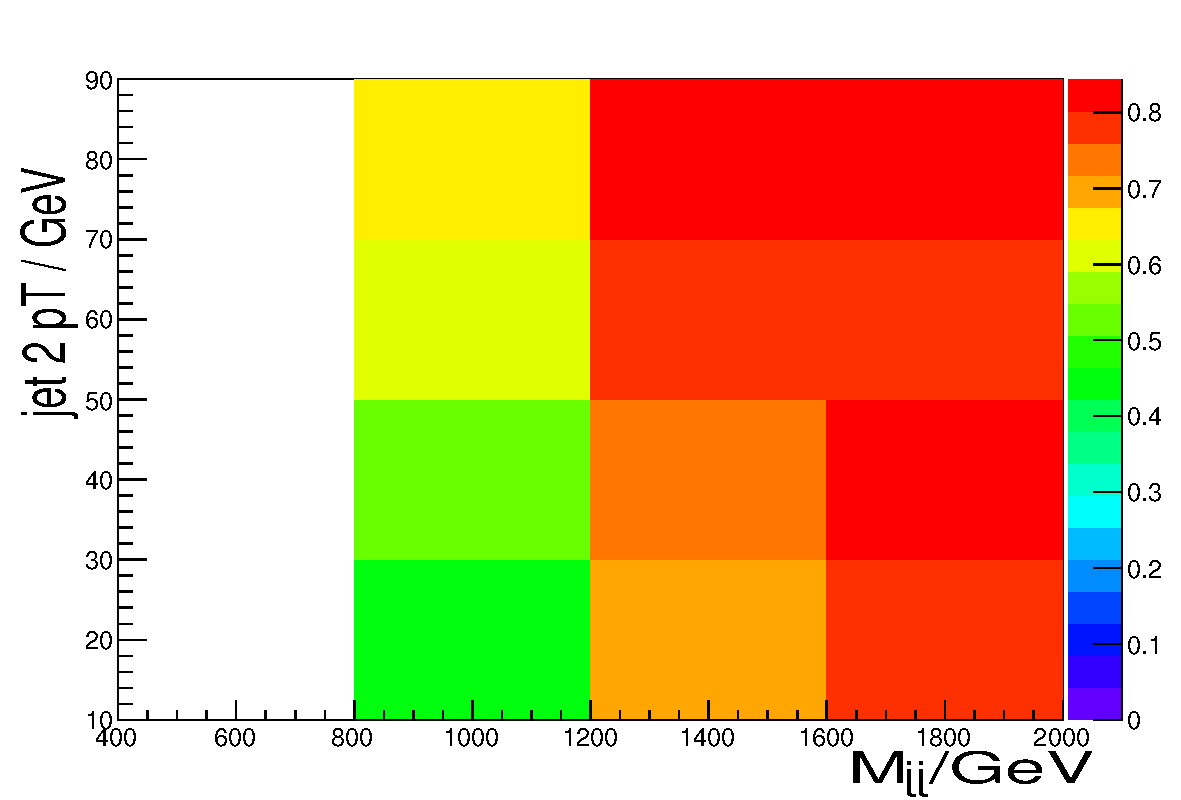
\includegraphics[width=.65\largefigwidth]{plots/parked/HLT_DiJet35_MJJ700_AllJets_DEta3p5_VBFmet120trigeff.pdf}}
  \subfloat[]{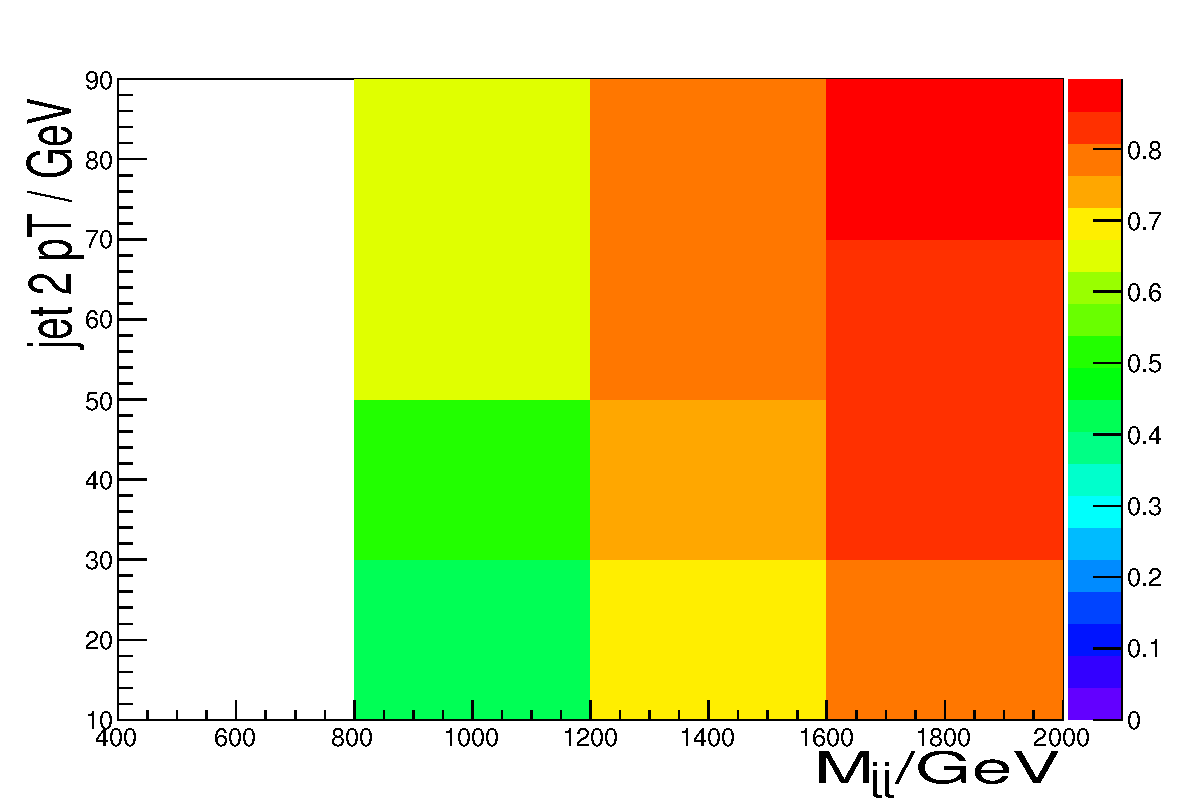
\includegraphics[width=.65\largefigwidth]{plots/parked/HLT_DiJet30_MJJ700_AllJets_DEta3p5_VBFmet120trigeff.pdf}}
 \caption{The efficiency for the trigger (color-scale) used in eras B and C (a) and era D (b), as a function of \Mjj and sub-leading jet \pt for events with \METnoMU between 60 and 120 \GeV. The efficiency was measured using a single muon dataset collected with an orthogonal trigger.}
  \label{fig:parked3dtrigeff}
\end{figure}

In order to achieve a smoother parameterisation of the trigger efficiency, coarse bins in \Mjj and sub-leading jet \pt were chosen, and a fit to the \METnoMU efficiency distribution in each bin was performed, using the following function:
\begin{equation}
  \label{eq:parkedtrigfunc}
  f\left(x\right)=\frac{A}{2}\cdot\left(1+ \frac{2}{\sqrt{\pi}}\int_{0}^{\frac{x-B}{\sqrt{C}}}e^{-t^{2}}\mathrm{d}t\right),
\end{equation}
which has a maximum value of A, and is derived from the error function with centre B and width related parameter C. The width, maximum and centre of the function are all allowed to float in the fit. The events used in this study were required to have leading jet \pt$>50$ \GeV, $\eta_{j1}\cdot\eta_{j2}<0$ and \detajj$>3.6$ to ensure that there are no inefficiencies due to these variables. The results of these fits for the two \Mjj and sub-leading jet \pt bins containing the most events entering the final analysis selection are shown in \FigureRef{fig:parkedtrigeff}. The fit can be seen to describe the data well and the uncertainties are small. The results for the remaining bins are shown in \AppendixRef{app:trigeffs}. Most bins have good agreement between the fit and the data, however, some of the plots in the appendix indicate that the parameters of the fit have taken extreme values, or have very large uncertainties. These extreme values and poor fits are mostly due to low numbers of events in the bin. The analysis selection described in \SectionRef{sec:parkedsel}, ensures that no events in these bins are used in the analysis.

\begin{figure}
  \subfloat[]{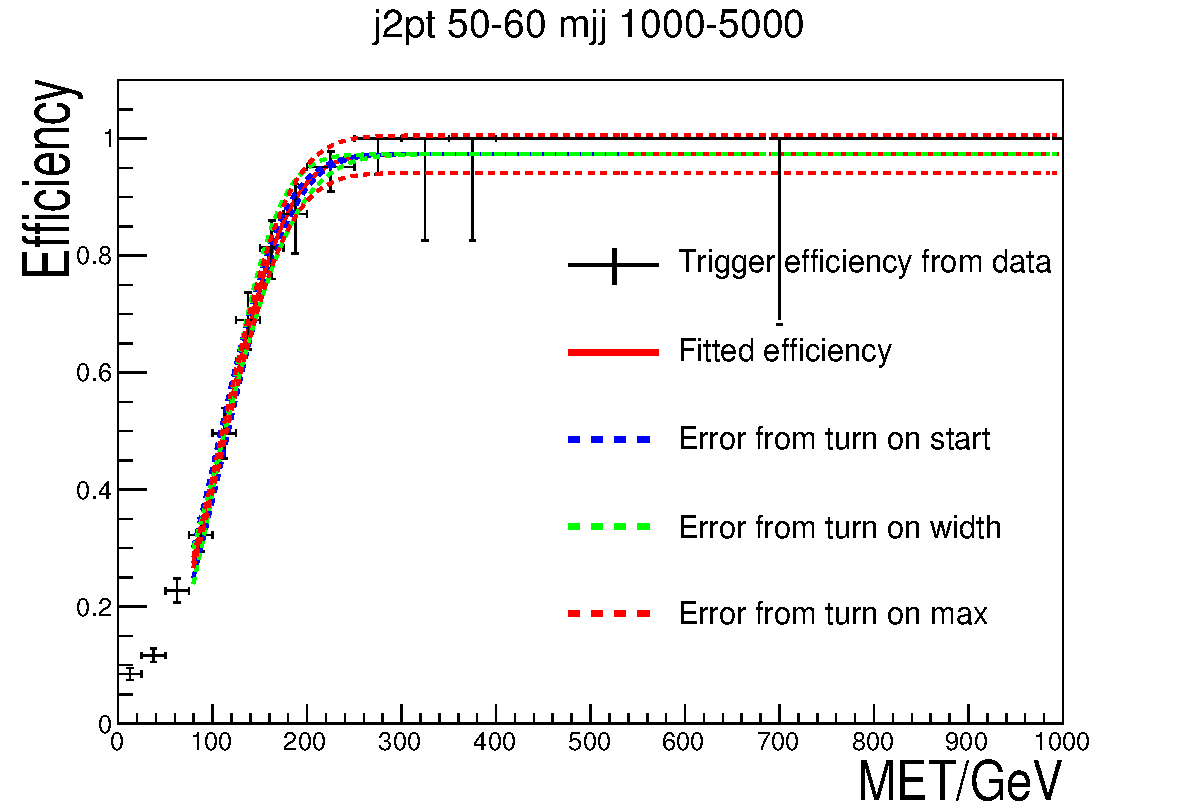
\includegraphics[width=.65\largefigwidth]{plots/parked/trigfitplots/hData_MET_1D_35D.pdf}}
  \subfloat[]{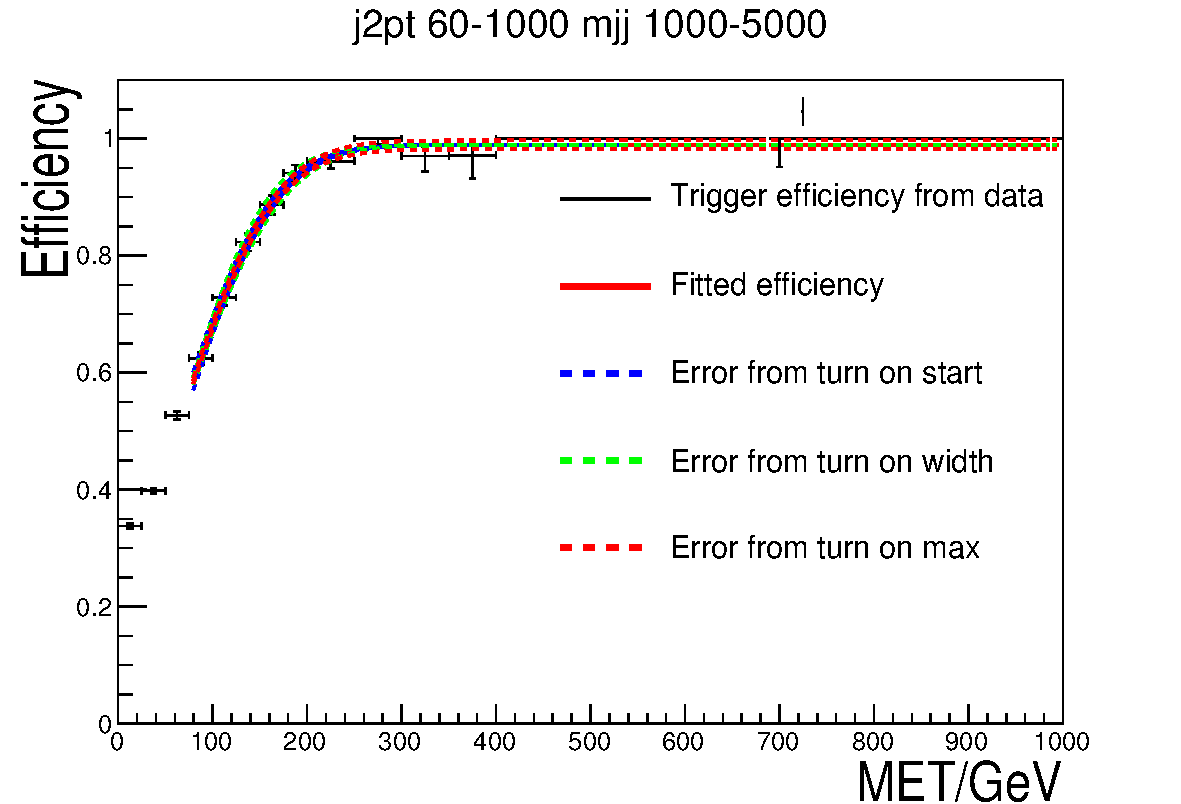
\includegraphics[width=.65\largefigwidth]{plots/parked/trigfitplots/hData_MET_1D_45D.pdf}}
  \caption{The results of performing a fit of the function in \EquationRef{eq:parkedtrigfunc} to the efficiency of the trigger used in era D, measured in a sample of single muon events collected with an orthogonal trigger. The dashed bands show the uncertainty on the fit due to each of the three parameters of the fit. The two bins of dijet mass (mjj) and sub-leading jet's \pt (j2pt) shown are those with the two highest numbers of events from the final signal region described in \SectionRef{sec:parkedsel}. The results of the fits in the other bins are shown in \AppendixRef{app:trigeffs}.}
  \label{fig:parkedtrigeff}
\end{figure}

Each \ac{MC} event was weighted by the average of the efficiency found for each of the three triggers weighted by the amount of integrated luminosity recorded using each trigger as shown in the following equation:
\begin{equation}
  \label{eq:parkedtrigweight}
  w\left(p_{\mathrm{T}j2},\Mjj,\METnoMU\right)=\frac{\sum_{i}\mathcal{L}_{i}\epsilon_{i}\left(p_{\mathrm{T}j2},\Mjj,\METnoMU\right)}{\sum_{i}\mathcal{L}_{i}},
\end{equation}
where $i$ are the three triggers, $\epsilon_{i}\left(p_{\mathrm{T}j2},\Mjj,\METnoMU\right)$ is the measured efficiency for trigger $i$ as a function of the event's sub-leading jet \pt, \Mjj and \METnoMU, and $\mathcal{L}_{i}$ is the integrated luminosity collected using trigger $i$. The resulting trigger efficiency varies smoothly and leads to no unphysical discontinuities in the distributions of event variables as can be seen from the figures in the remainder of this chapter.

\section{Event selection}
\label{sec:parkedsel}
As mentioned above a significant challenge in the analysis of the parked data is that the additional areas of phase space collected by these triggers, but not collected by the prompt data triggers, have very large contributions from \ac{QCD} backgrounds. The \ac{QCD} contribution to \ac{VBF} analyses is very hard to model because although the cross-sections for these processes are very high, the probability of any individual event being \ac{VBF}-like is very low. The number of \ac{MC} events that must be generated to make a representative sample is therefore prohibitively large. As a result of these difficulties, the parked data selection is separated into two stages. The first ``preselection'' stage selects a region of phase space which is not expected to be dominated by \ac{QCD} processes. After this preselection has been made the background processes expected to contribute are the same as in the prompt analysis, and studies were undertaken into which background estimation methods and final signal region selection leads to the best expected limit.

%runcbug101114.pdf sig reg optimisation

\subsection{Preselection}
\label{sec:parkedpresel}
The first element of the preselection was motivated by the trigger. The following selection was applied to ensure that the values of all event variables are above the trigger thresholds of all triggers used, and that the \METnoMU was above the lowest value of the turn on centre, B, as defined in \EquationRef{eq:parkedtrigfunc}, obtained from the fits described in \SectionRef{sec:parkedtrigger}:
\begin{align}
  \label{eq:parkedprepresel}
  \begin{split}
  \eta_{j1}\cdot\eta_{j2}<0,\,\mathrm{leading\,jet\,}\pt>50 \GeV, \detajj>3.6, \\
  \mathrm{sub-leading\,jet\,}\pt>40 \GeV, \Mjj>800 GeV, \METnoMU>90\GeV.
  \end{split}
\end{align}
Where $j1$ and $j2$ are the leading and sub-leading \pt jets in the event and are chosen as the \ac{VBF} tag jets. We also require that for the ``signal-like'' selection there are no veto electrons or muons in the event. The W+jets and Z+jets control regions used in the background estimates described in \SectionRef{sec:parkedbkg} impose different lepton requirements. QCD multijet processes still dominate the region defined by this selection, as can be seen in \FigureRef{fig:parkedpresel}a, where there are a lot more data events than expected from the background \ac{MC} prediction. This difference is due to mismeasured \ac{QCD} events not being adequately modelled by the available \ac{MC} samples, which are described in further detail in \SectionRef{sec:parkedQCD}. 

Additional selection requirements were applied to reduce the observed differences from the mismeasured \ac{QCD} multijet background. The first variable that was used to achieve this reduction is the \MET significance, \METsig, which is defined as the ratio between \METnoMU and the square root of the sum of the transverse energy of all particles in the event, which is an estimate of the statistical error on the \MET. As the sum of the square root of the transverse energy of all particles is being used as an estimate of the statistical uncertainty on the \MET it has units of \GeV and \METsig is therefore unitless. The intention of the \METsig cut is to remove events which have a large amount of \MET, but also have an even larger amount of visible energy, meaning that the \MET is likely to be from mismeasurement of the visible particles. The preselection requires that \METsig be greater than 3. The value of this cut was chosen by looking at \FigureRef{fig:parkedpresel}a and removing the region with the most disagreement between data and \ac{MC}. The resulting region shown in \FigureRef{fig:parkedpresel}b still does not display good data-\ac{MC} agreement, however the disagreement is smaller.

After the cut on \METsig, a requirement that the \METnoMU is not too close to any jets in \phi was made. This requirement was motivated by the fact that if the \MET is due only to the mismeasurement of a jet, the \MET will be aligned with that jet. Two variables were investigated, the first was the minimum azimuthal angle difference between either of the two tag jets and the \METnoMU, \jetmetdphileading, and the second was the minimum azimuthal angle difference between any jet with \pt greater than 30 \GeV and the \METnoMU, \jetmetdphi. At a similar signal efficiency the difference between the observed number of events and the \ac{MC} background prediction, which is an indication of the remaining \ac{QCD} multijet background, was found to be 80\% smaller for a cut on \jetmetdphi than a cut on \jetmetdphileading. The same cut on \jetmetdphi was also found to reduce top quark related backgrounds by a factor of two compared to a cut on \jetmetdphileading. We therefore require that \jetmetdphi$>1.0$ for events to pass the preselection. \jetmetdphi was found to give significantly better signal efficiency than the \dphijj variable used in the prompt analysis for the same background rejection, so no cut was made on \dphijj.

%AN-14-243
\begin{figure}
  \subfloat[]{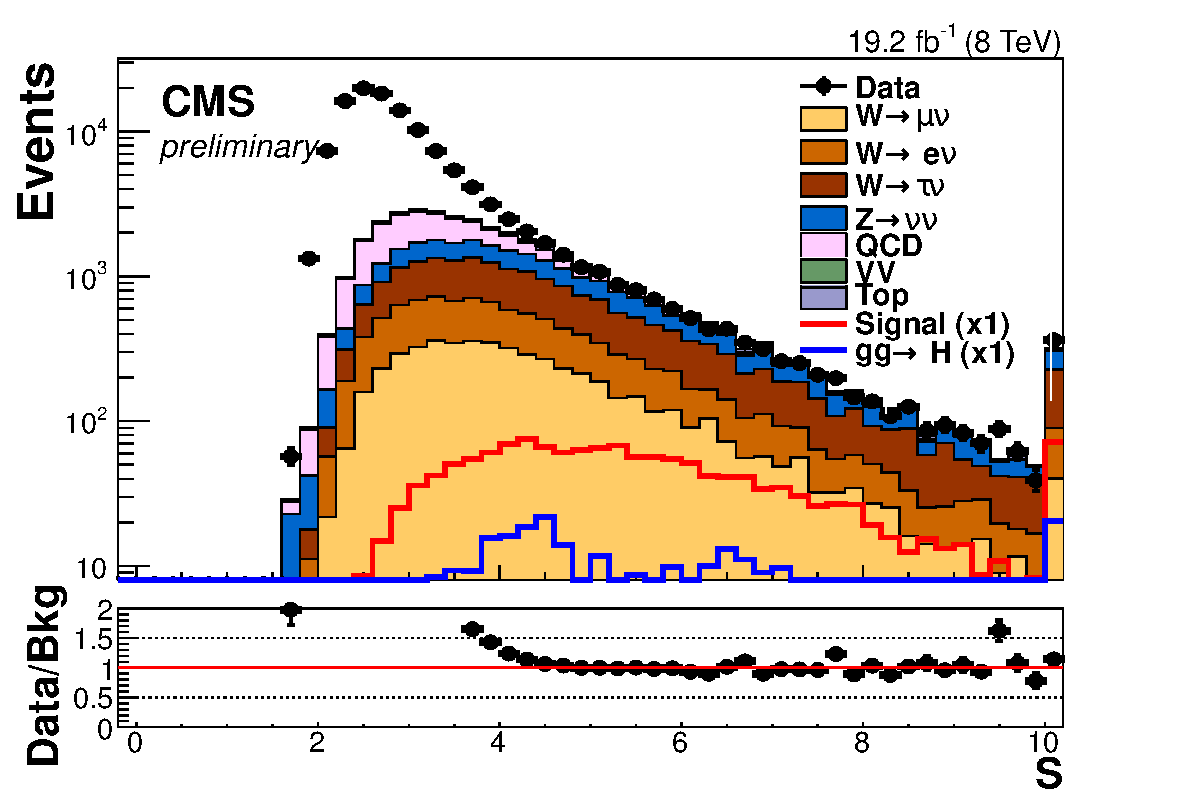
\includegraphics[width=.7\largefigwidth]{plots/parked/AN-14-243-figs/lognopreselnunu_metnomu_significance.pdf}}
  \subfloat[]{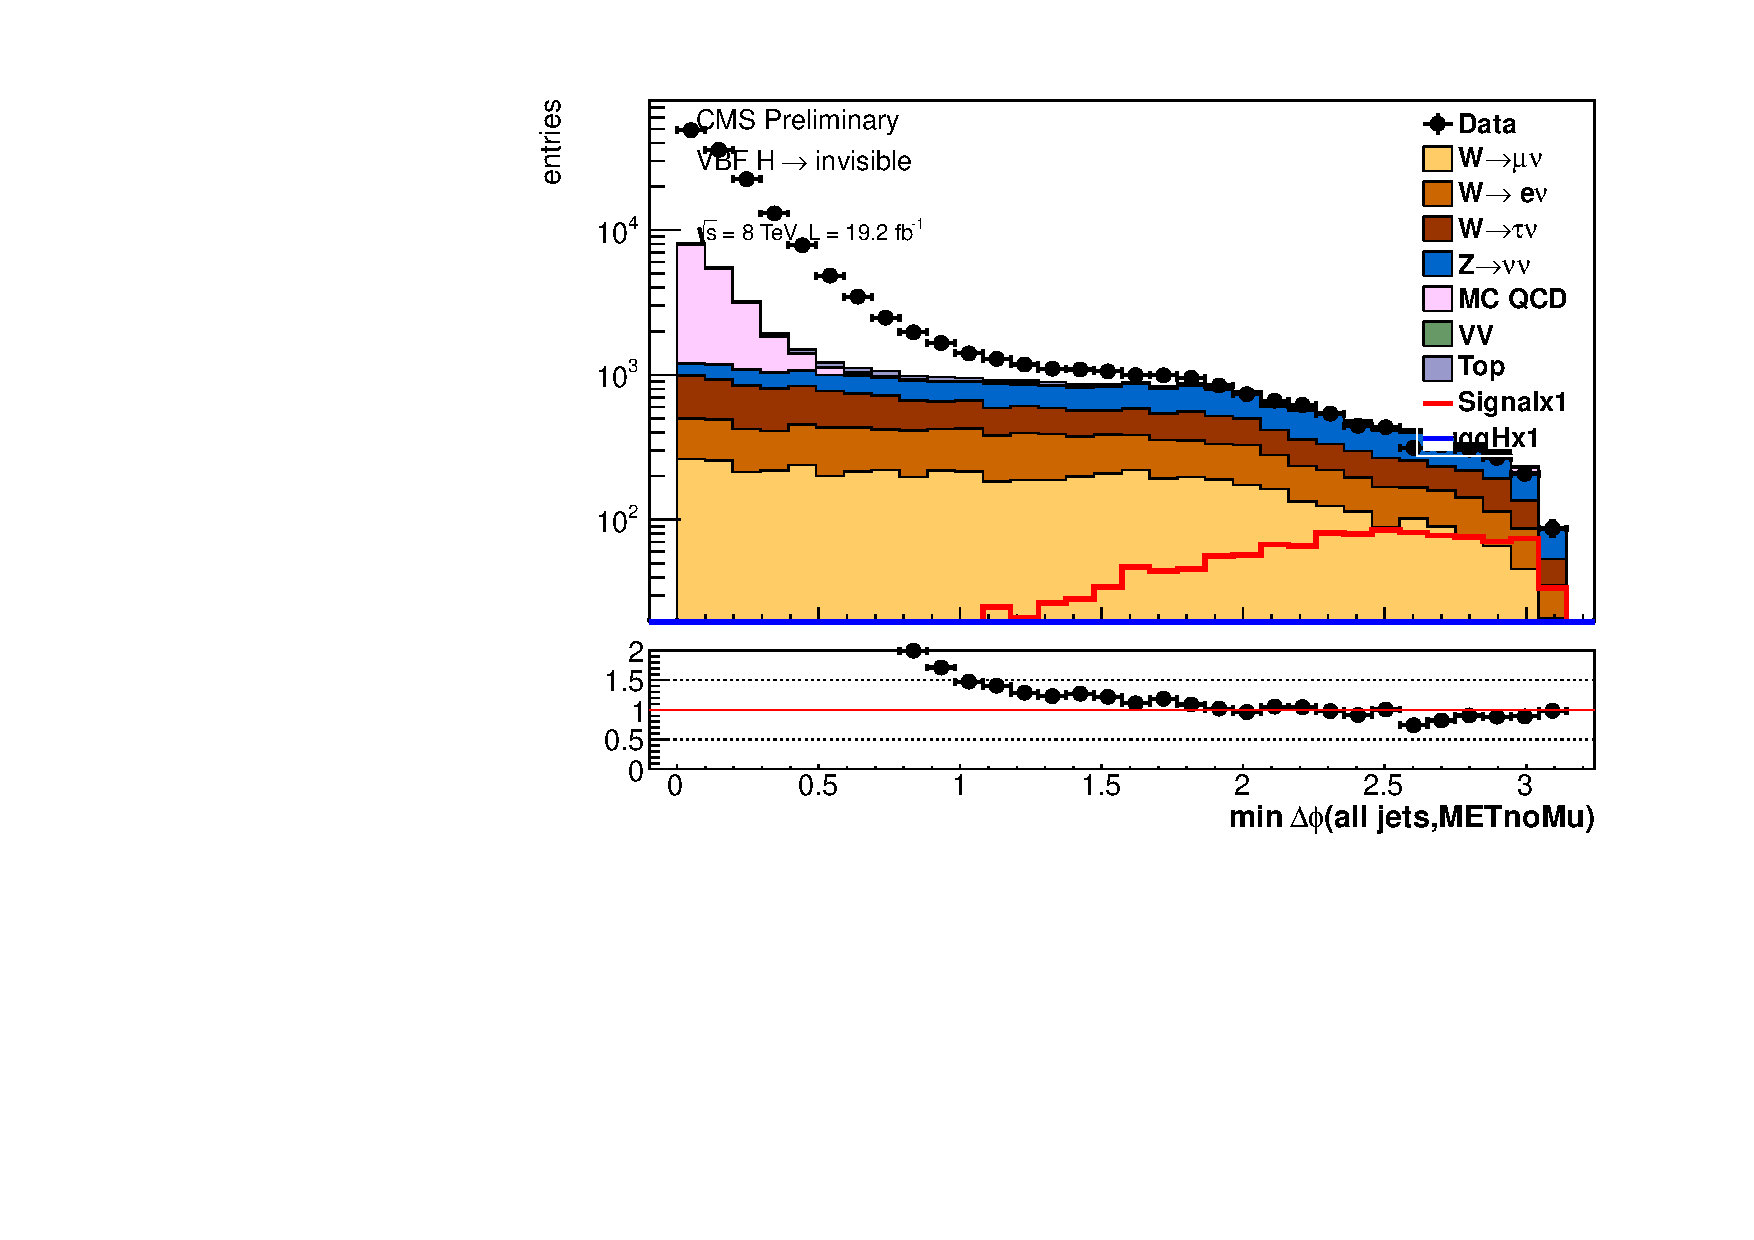
\includegraphics[width=.7\largefigwidth]{plots/parked/AN-14-243-figs/logmetsigpreselnunu_alljetsmetnomu_mindphi.pdf}}

  \subfloat[]{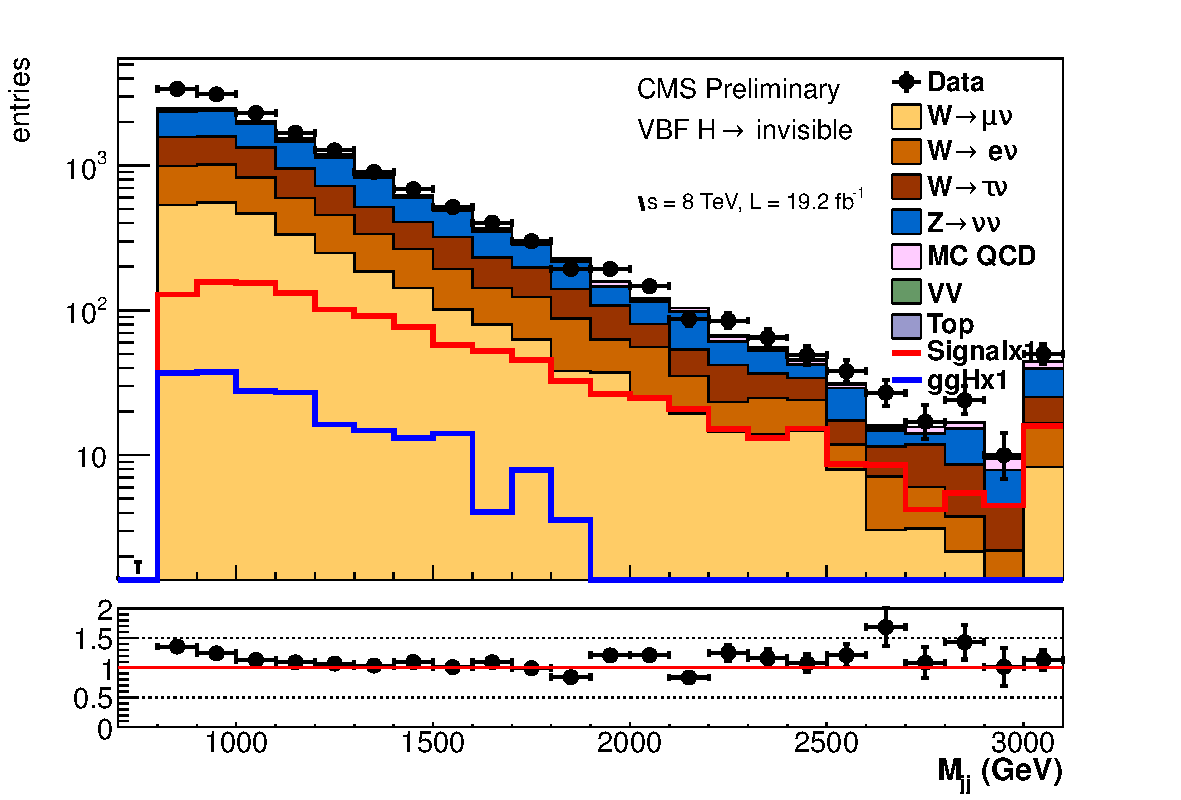
\includegraphics[width=.7\largefigwidth]{plots/parked/AN-14-243-figs/logmjj800nunu_dijet_M.pdf}}
  \caption{(a) \METsig after the trigger driven selection described in \EquationRef{eq:parkedprepresel}. (b) \jetmetdphi after the trigger driven selection and requiring \METsig$>3$. (c) \Mjj after the trigger driven selection and requiring \METsig$>3$ and \jetmetdphi$>1$. All three plots are of the signal-like region with the \ac{MC} scaled using the background estimation methods described in \SectionRef{sec:parkedbkg}. The disagreement between data and the predictions from background \ac{MC} samples is believed to be due to mismeasured \ac{QCD} multijet events which are not well modelled by the available \ac{MC} samples. The last bin of each distribution contains the events above the range displayed. Signal (gg$\rightarrow$H) refers to an \ac{SM} \ac{VBF} (\ac{ggH}) produced Higgs boson with \BRinv=100\%.}
  \label{fig:parkedpresel}
\end{figure}

%contplotsandpresel160914
The \Mjj distribution after the \jetmetdphi cut is shown in \FigureRef{fig:parkedpresel}c. Whilst the agreement for large \Mjj is good, it can be seen that the first bin of the distribution, where mismeasured \ac{QCD} multijet events would be expected, due to them not recoiling against another object, shows a significant disagreement. The final cut of the preselection is therefore to require \Mjj$>1000$ \GeV. This cut also ensures that none of the bins used to describe the trigger efficiency which have too few events to be reliable are used. In summary the full preselection is as follows:
\begin{equation}
  \label{eq:presel}
  \begin{split}
  \eta_{j1}\cdot\eta_{j2}<0,\,\mathrm{leading\,jet\,}\pt>50 \GeV, \detajj>3.6, \\
  \mathrm{sub-leading\,jet\,}\pt>40 \GeV, \Mjj>1000 GeV, \METnoMU>90\GeV, \\
  \jetmetdphi>1.0, \METsig>3.0.
  \end{split}
\end{equation}
Distributions of several variables after the full preselection are shown in \FigureRef{fig:parkedpostpresel}. No estimate of the \ac{QCD} contribution is given in these distributions, and it can be seen that there is still disagreement between data and \ac{MC} in the areas where \ac{QCD} would be expected to contribute. Further selection is, therefore, necessary.

\begin{figure}
  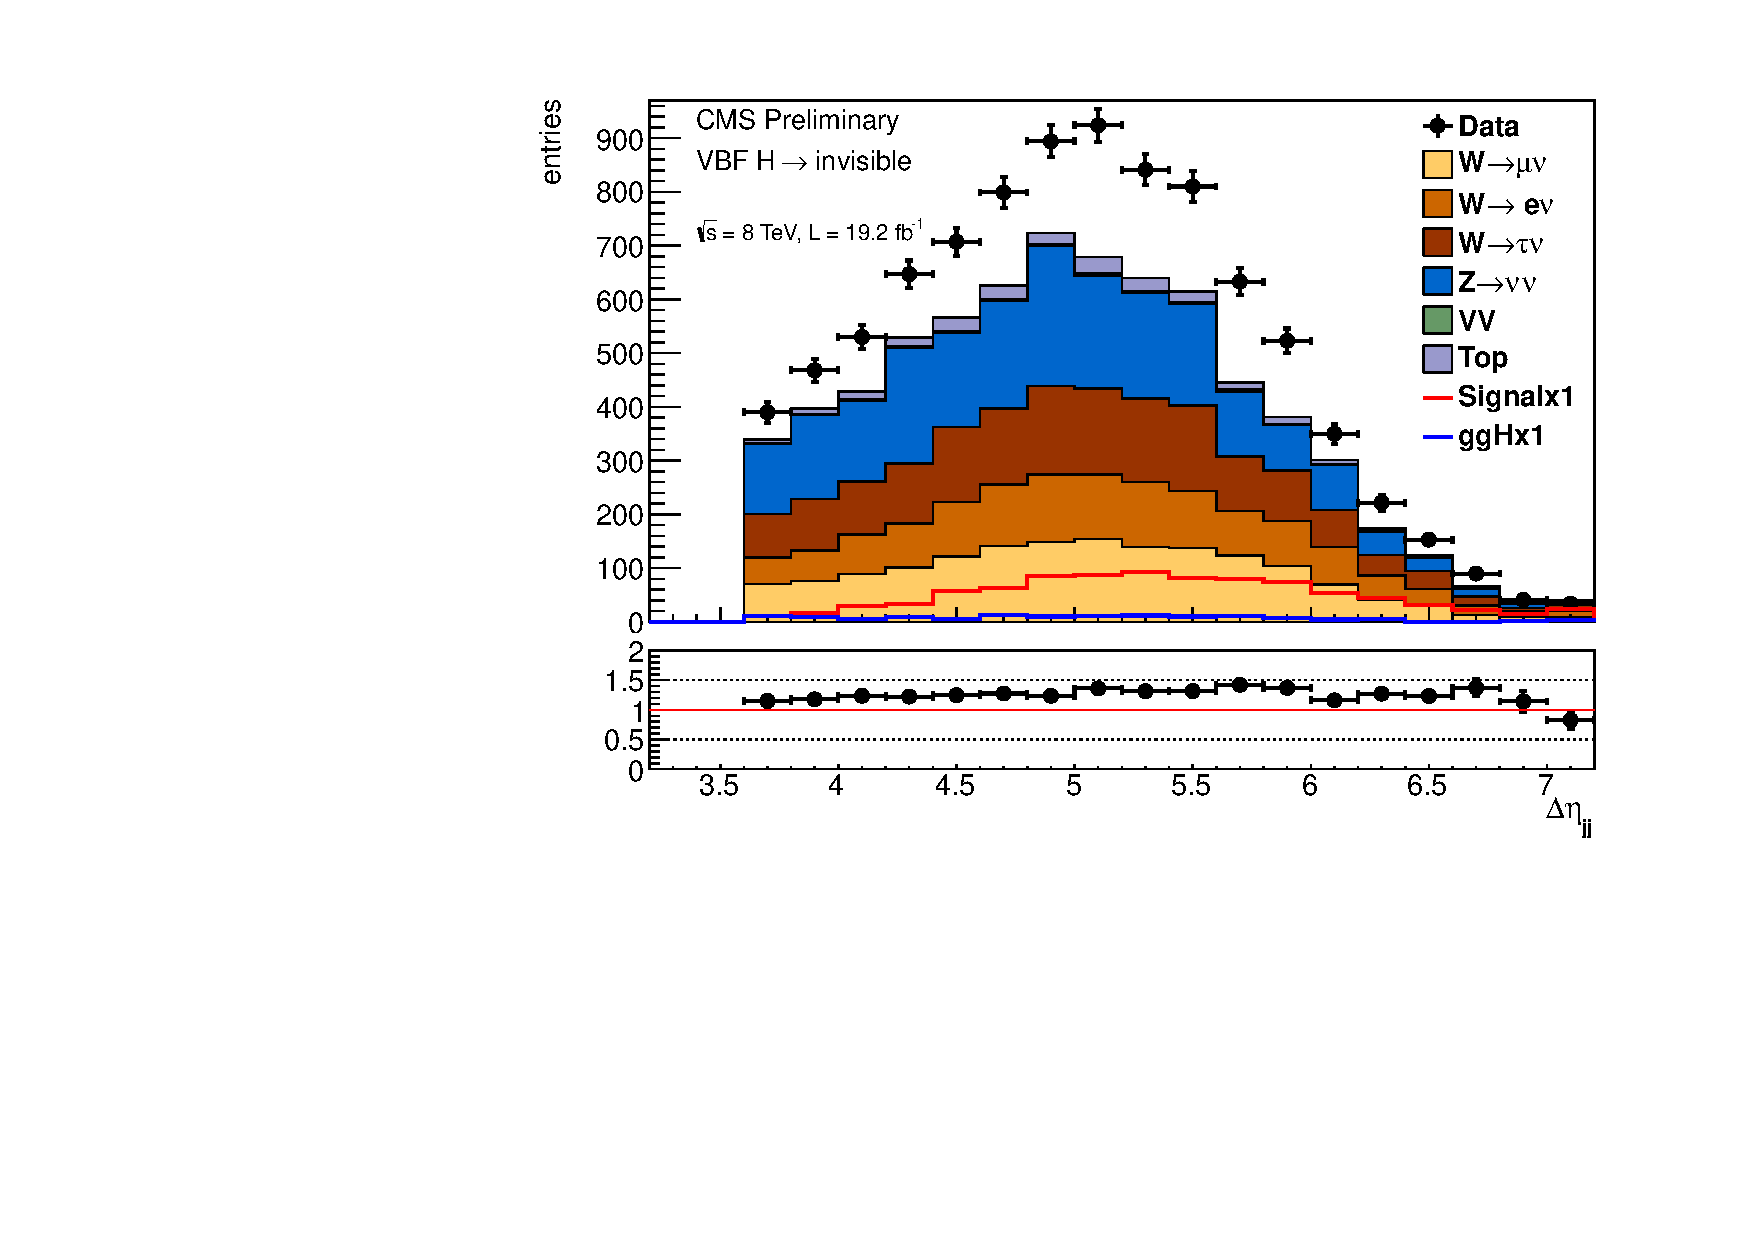
\includegraphics[width=.65\largefigwidth]{plots/parked/AN-14-243-figs/output_presel/nunu_dijet_deta.pdf}
  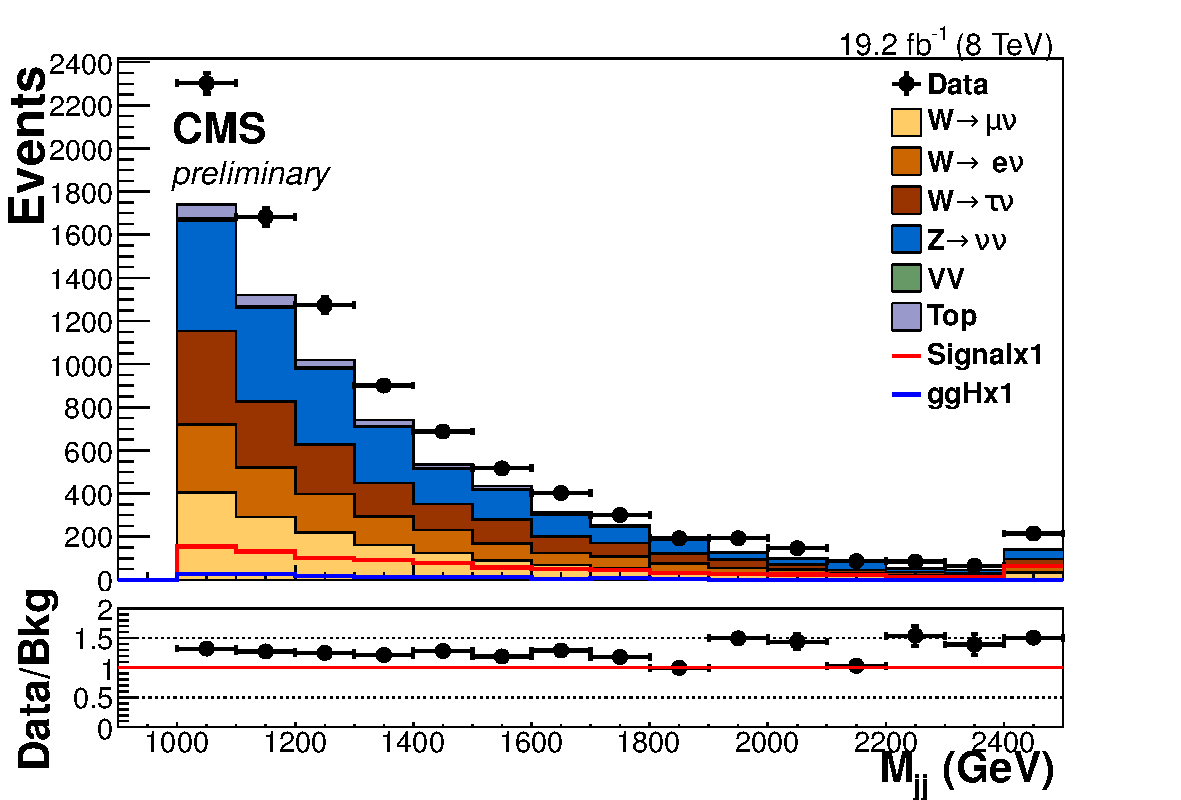
\includegraphics[width=.65\largefigwidth]{plots/parked/AN-14-243-figs/output_presel/nunu_dijet_M.pdf}
  
  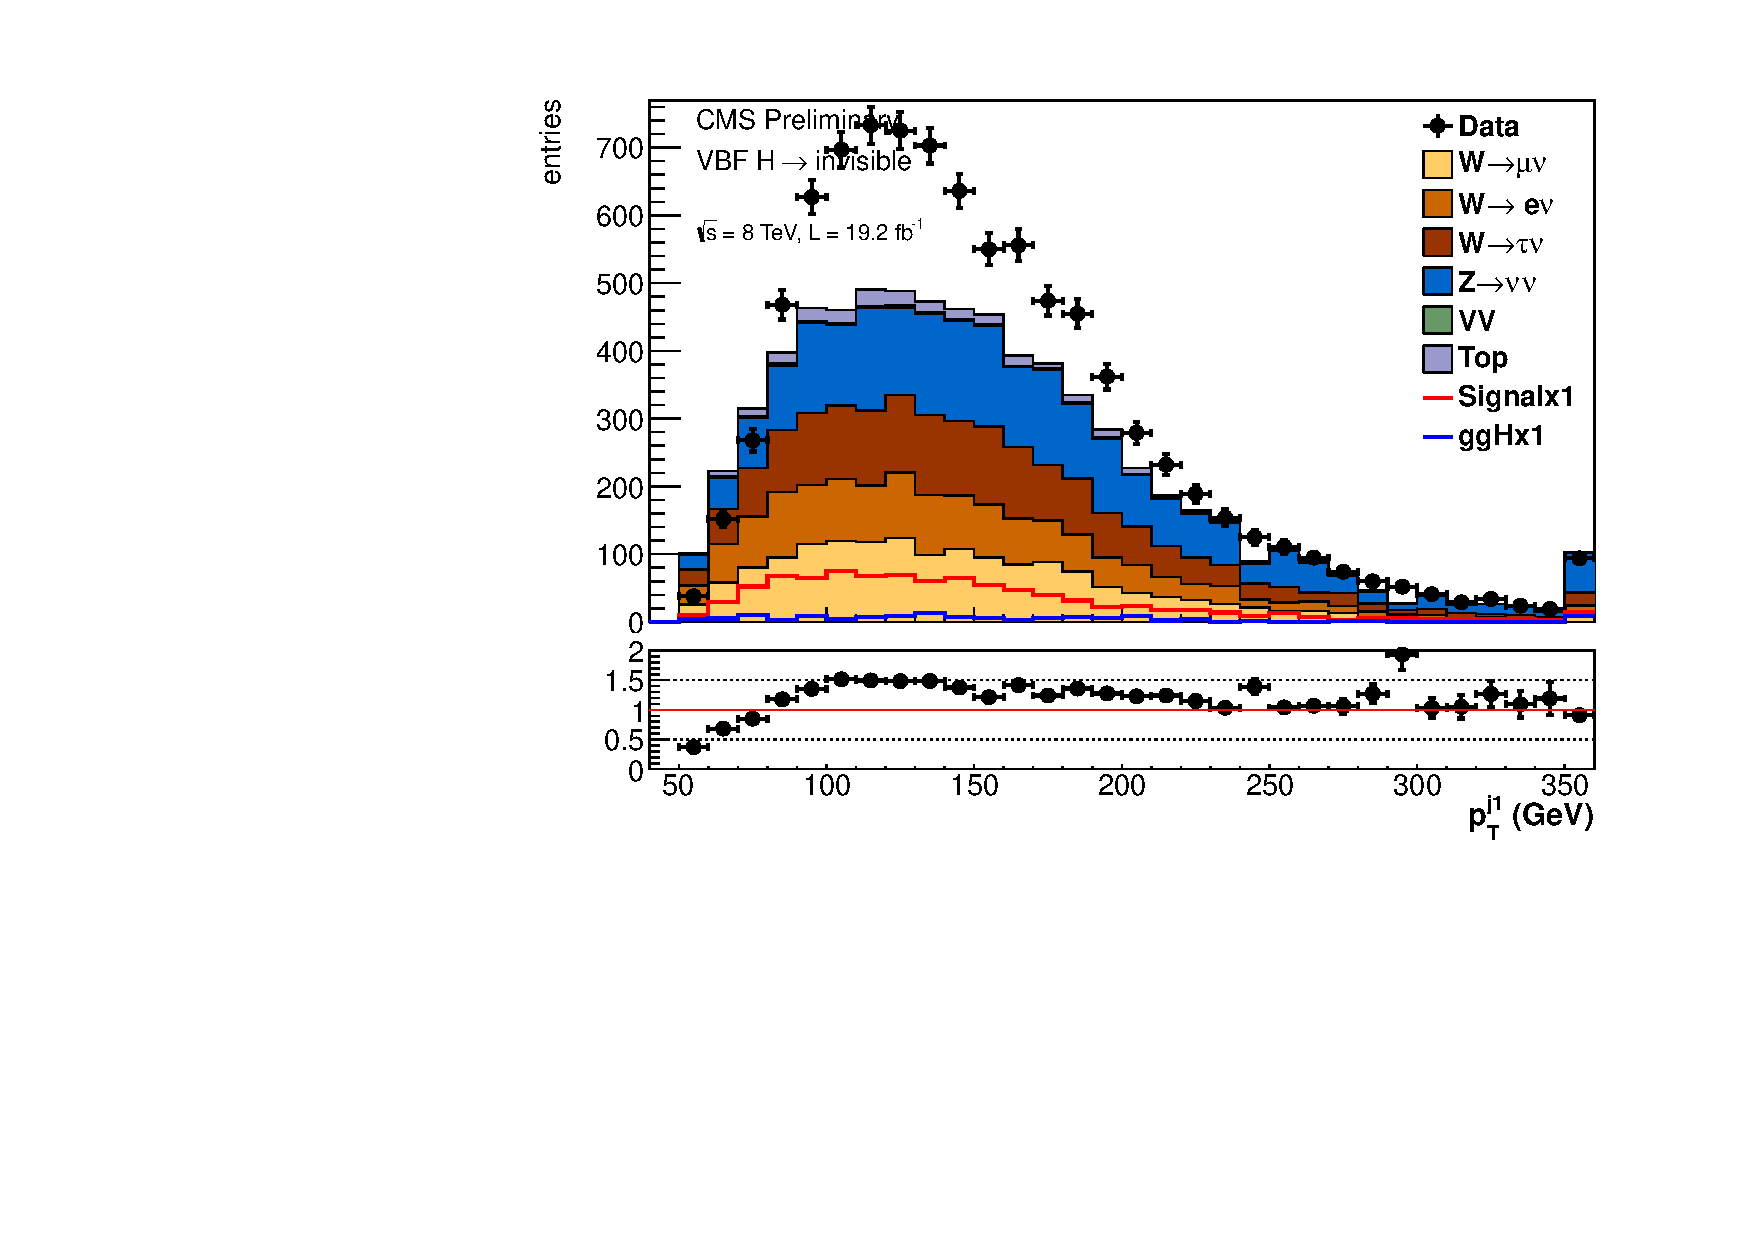
\includegraphics[width=.65\largefigwidth]{plots/parked/AN-14-243-figs/output_presel/nunu_jet1_pt.pdf}
  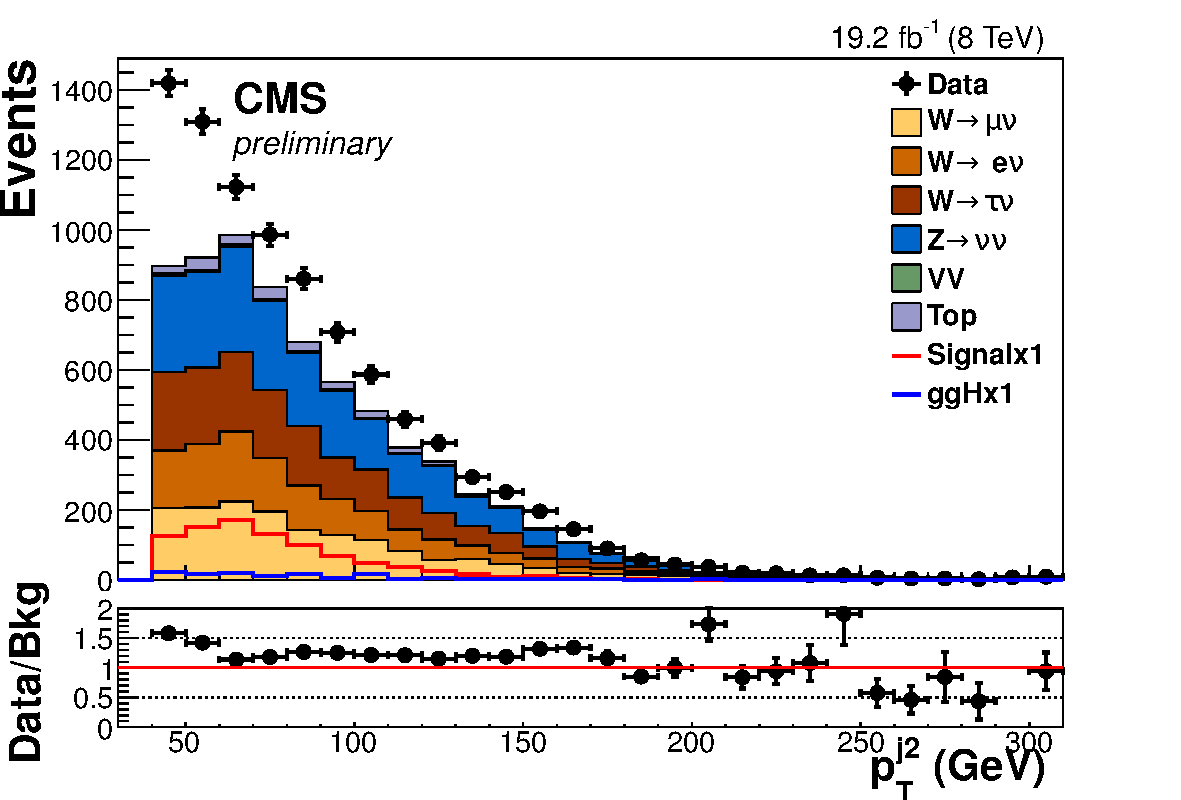
\includegraphics[width=.65\largefigwidth]{plots/parked/AN-14-243-figs/output_presel/nunu_jet2_pt.pdf}

  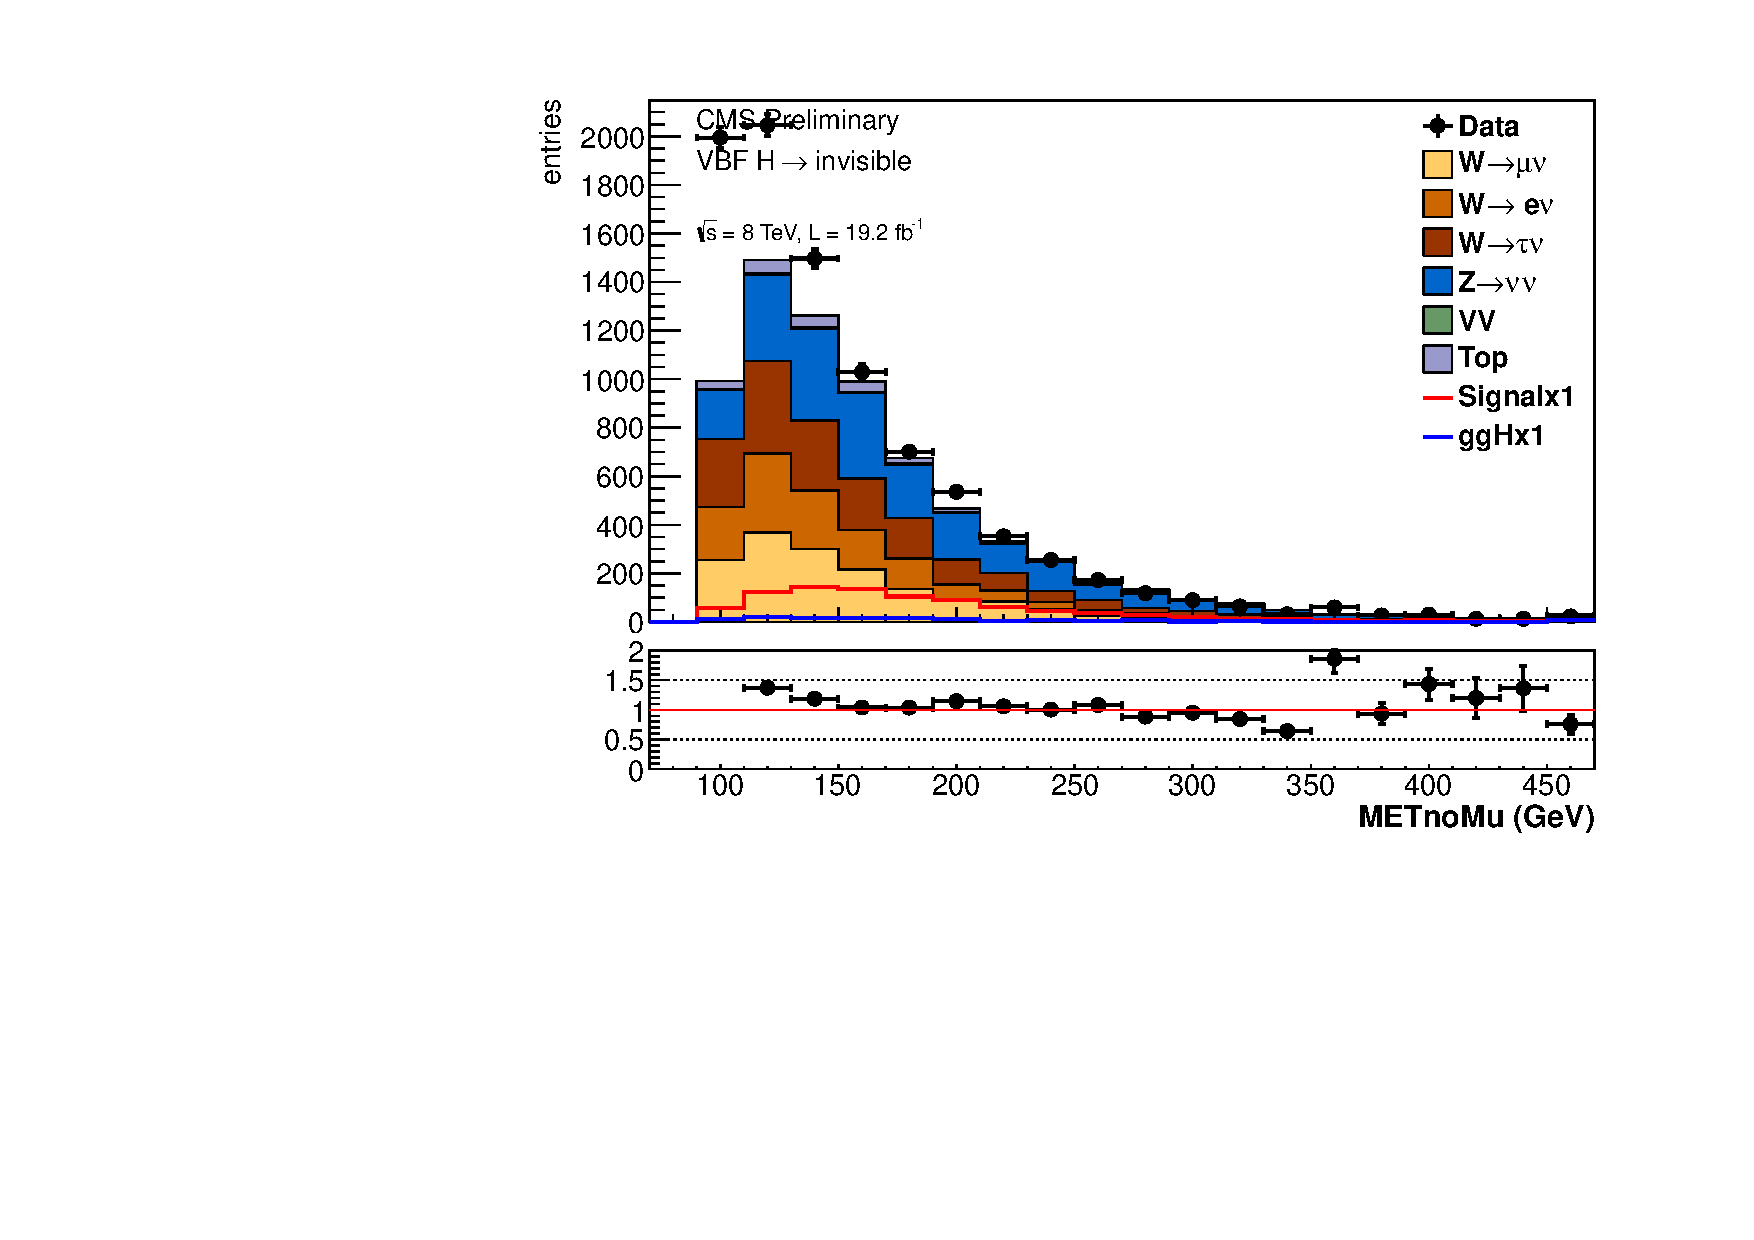
\includegraphics[width=.65\largefigwidth]{plots/parked/AN-14-243-figs/output_presel/nunu_metnomuons.pdf}
  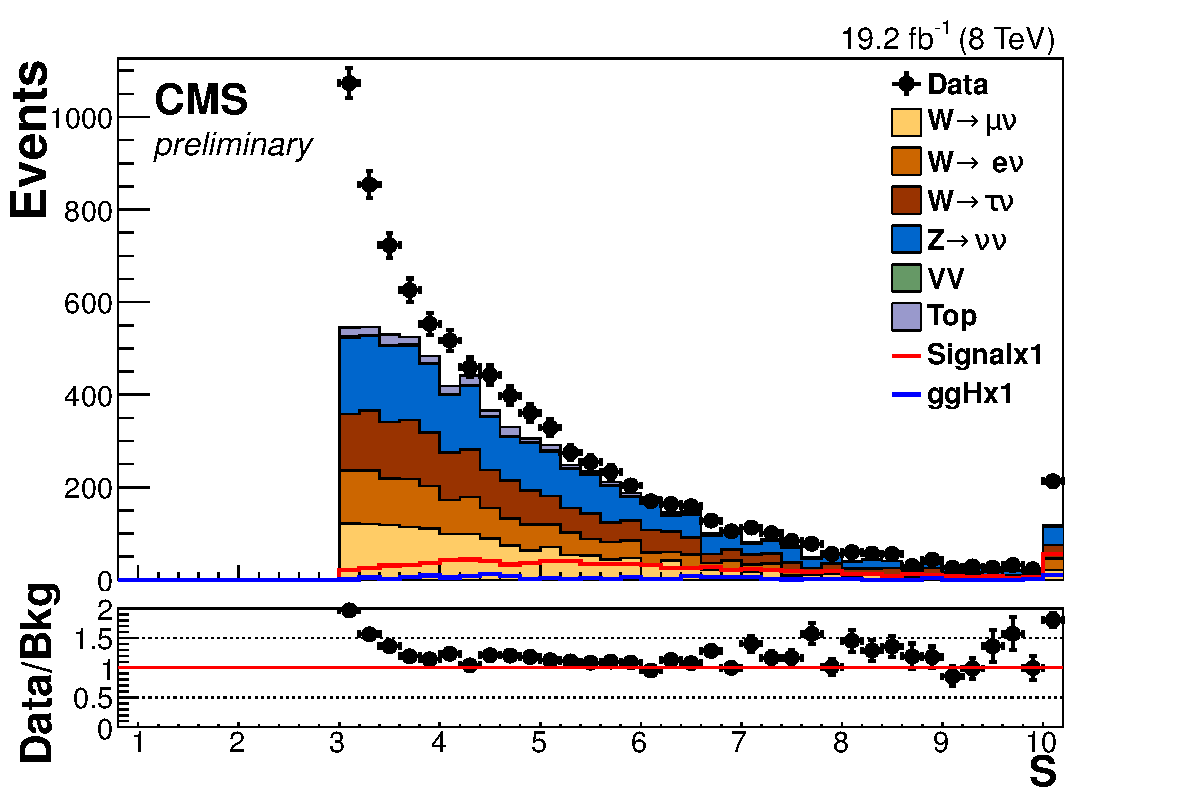
\includegraphics[width=.65\largefigwidth]{plots/parked/AN-14-243-figs/output_presel/nunu_metnomu_significance.pdf}
  
  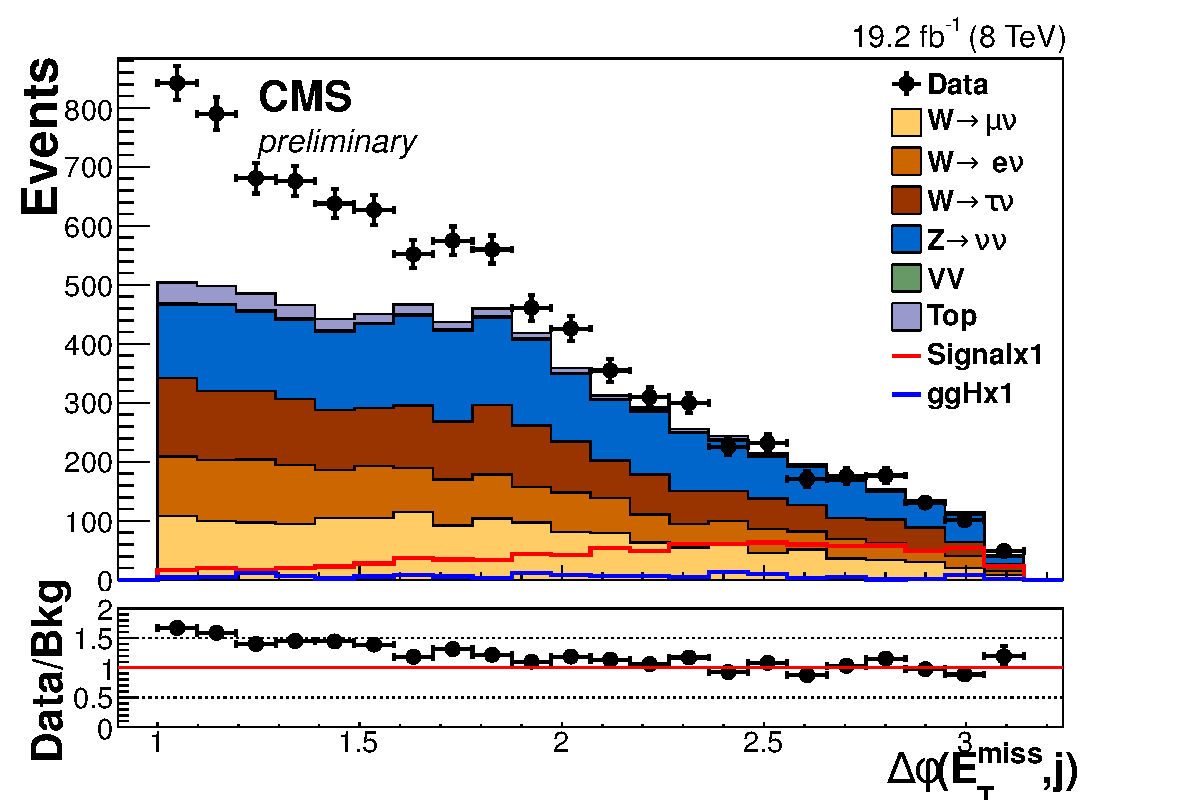
\includegraphics[width=.65\largefigwidth]{plots/parked/AN-14-243-figs/output_presel/nunu_alljetsmetnomu_mindphi.pdf}

  \caption{From top to bottom, left to right, distributions of \detajj, \Mjj, leading jet \pt, sub-leading jet \pt, \METnoMU, \METsig and \jetmetdphi for events passing the full preselection. No \ac{QCD} contribution is shown, which accounts for the difference between the data observation and background prediction. The last bin of each distribution contains the events above the range displayed.}
  \label{fig:parkedpostpresel}
\end{figure}




\subsection{Signal region selection}
\label{sec:parkedsigsel}
As can be seen from \FigureRef{fig:parkedpostpresel}, there is still a significant difference between the data and the \ac{MC} background prediction. It is also evident that the main areas where disagreement occurs are where contributions from \ac{QCD} backgrounds (which are not included in the figure) would be expected to contribute, at low \METsig and low \jetmetdphi, i.e. with jets close to the \METnoMU. Outside these \ac{QCD}-like regions good agreement between data and \ac{MC} is seen, indicating very low numbers of \ac{QCD} events remaining. The approach taken was to place tight requirements on these two variables to reduce the \ac{QCD} background to be much smaller than the other backgrounds considered. The large uncertainty on any estimate of the number of events from \ac{QCD} multijet processes therefore also becomes negligible. A requirement that events have $\jetmetdphi>2$ and $\METsig>4$, was therefore imposed. The resulting relatively \ac{QCD}-free ``optimisation'' region was blinded (i.e. the data were not looked at) to use for studies to determine the final signal region selection. All of the studies described in this chapter from this point until the results section were performed blind unless stated otherwise.

Two methods to select the signal region were investigated. The first method was a cut based selection. Starting from the optimisation region the cuts on \METsig, \jetmetdphi, \detajj, sub-leading jet \pt and \Mjj were varied one at a time and the expected limit for each combination of cuts was calculated. The method described in \SectionRef{sec:stats} was used, with the background estimation techniques and systematic uncertainties described in Sections~\ref{sec:parkedbkg} and \ref{sec:parkedsyst} respectively, to calculate the expected limit. In the case of the \ac{QCD} background, which has only a very small contribution to the signal region, the background estimation was performed once for the optimisation selection and used for all cut values. The estimations for all other background processes were repeated for each set of cuts. After each variable was varied the selection was updated to use the cut value that gave the best expected limit. After all the variables had been varied the process was repeated until no improvement in the expected limit was seen so as to avoid ignoring other better sets of cuts. The cut values that gave the best expected limit define the signal region and are as follows:
\begin{equation}
  \label{eq:parkedsigsel}
  \begin{split}
    \eta_{j1}\cdot\eta_{j2}<0,\detajj>3.6,\,\mathrm{leading\,jet\,\pt}>50 \GeV,\\
    \mathrm{sub-leading\,jet\,\pt}>45 \GeV, \Mjj>1200 \GeV,\\
    \METnoMU>90 \GeV, \METsig>4.0,\jetmetdphi>2.3.
  \end{split}
\end{equation}
After this selection was defined a second \ac{MVA} based method of optimising the selection was investigated to see if we could improve on the cut based selection. \ac{BDT} and Fisher discriminants were trained using signal and background events passing the signal region selection~\cite{TMVA}. The signal region selection was used as the basis for this training so as to ensure that the number of events from the \ac{QCD} background in the studied region was small. The optimisation procedure defined above was then repeated with the value of the discriminant considered as an additional variable. One advantage of \ac{MVA} based selection over simple rectangular cut based selection is that information about the correlation between variables is taken into account. The correlation coefficients between the variables used as inputs to the \ac{MVA} are shown for signal and V+jets background events in \FigureRef{fig:parkedmvacorr}. These variables were chosen as they showed the most difference between signal and background distributions and correlations out of a wide range of variables investigated. Without the addition of any additional systematic uncertainties associated with the understanding of the variables input to the \ac{MVA}, the largest improvement in the expected limit was less than 1\%. It was therefore decided to use the cut based selection as the final event selection.
\begin{figure}
  \subfloat[]{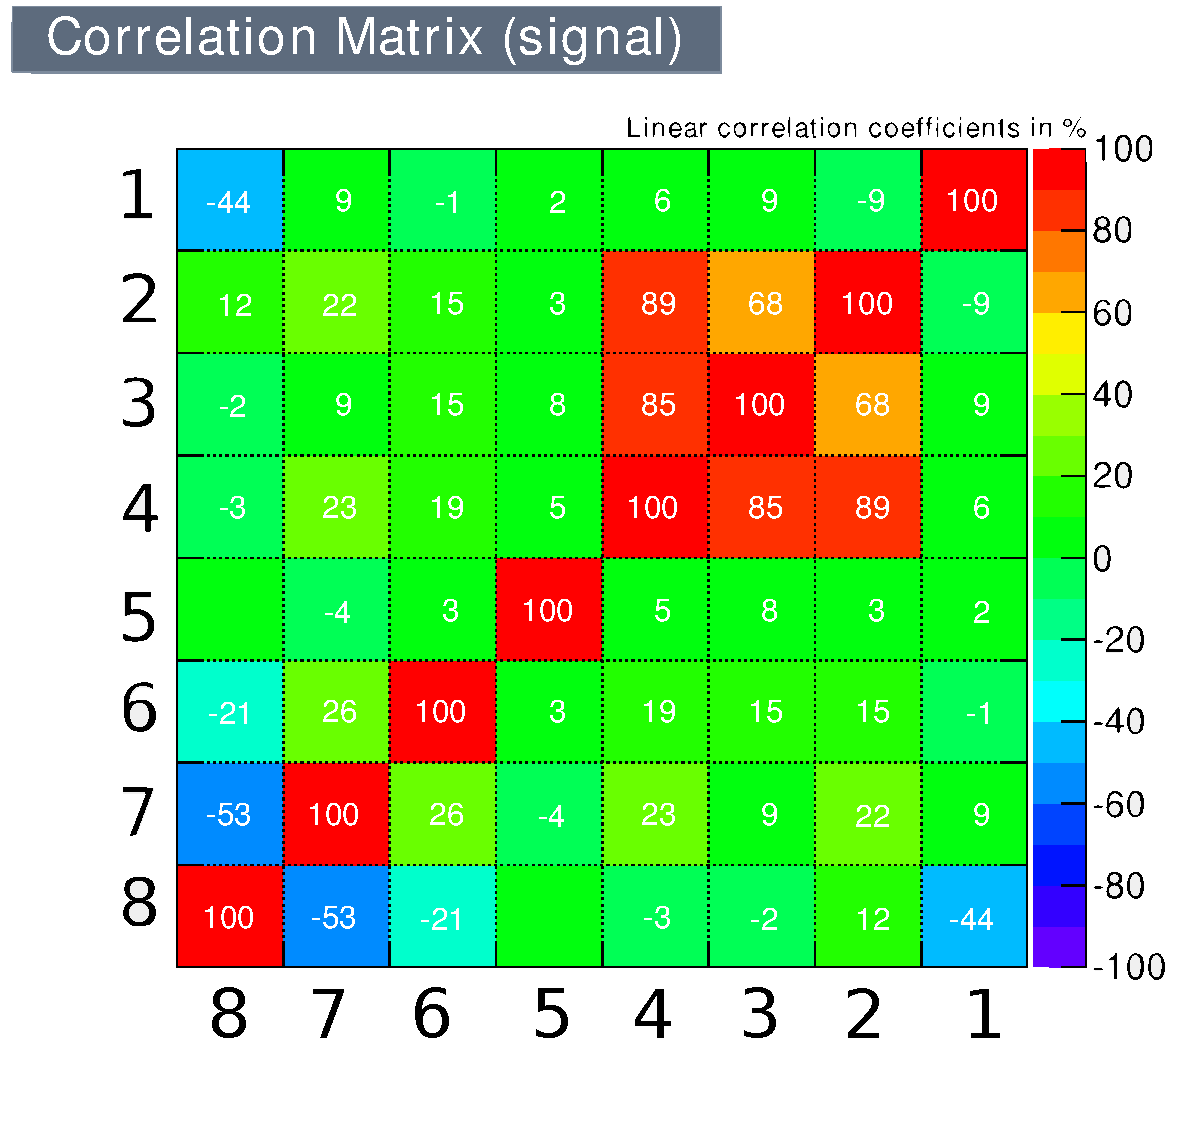
\includegraphics[width=.65\largefigwidth]{plots/parked/AN-14-243-figs/inputcorrsig.pdf}}
  \subfloat[]{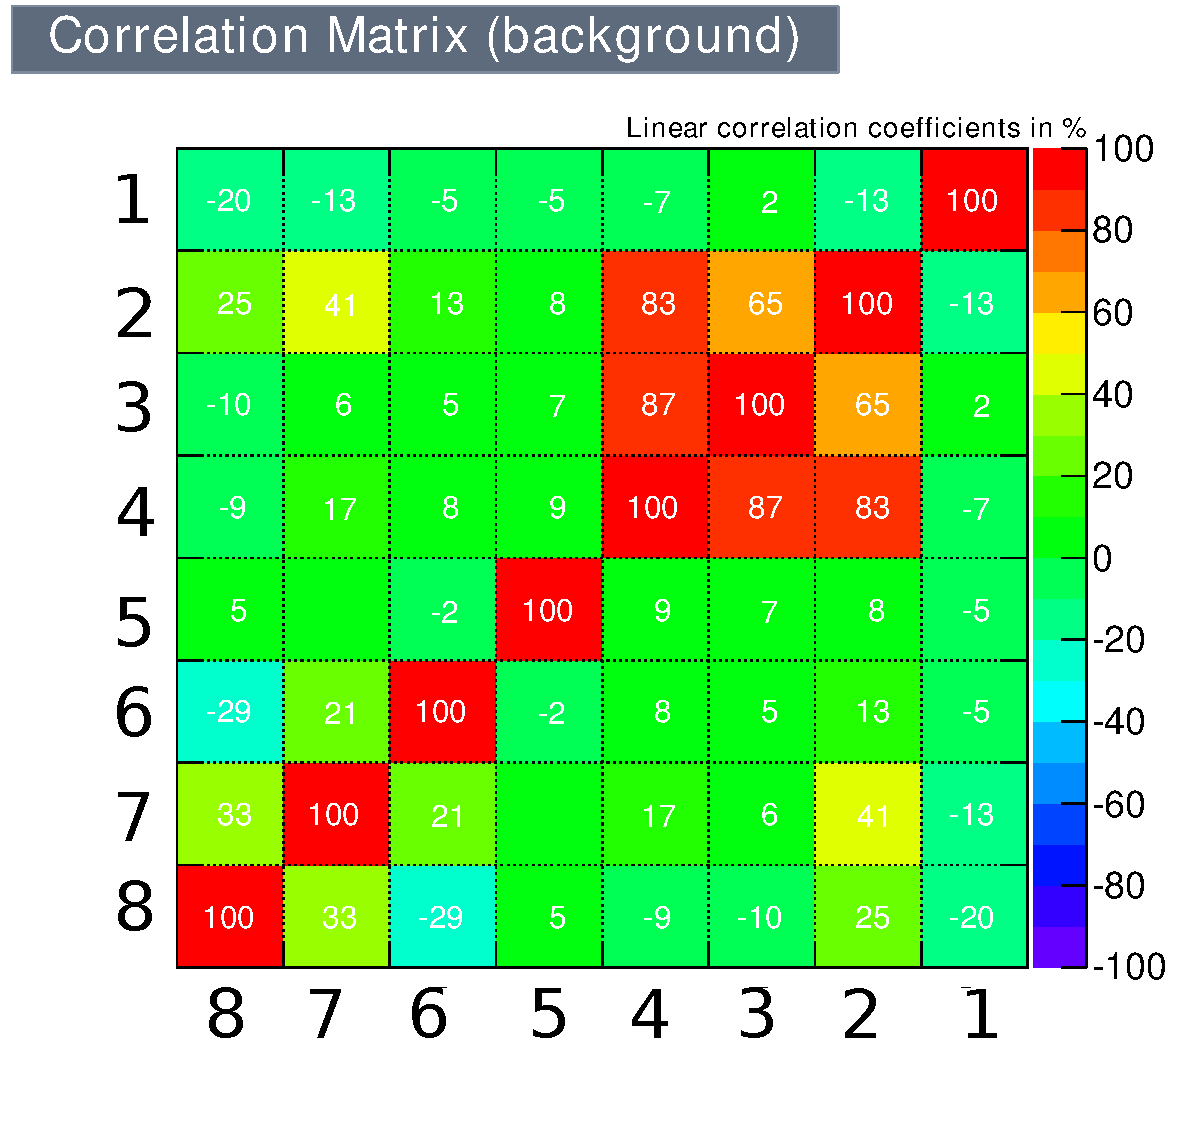
\includegraphics[width=.65\largefigwidth]{plots/parked/AN-14-243-figs/inputcorrbkg.pdf}}
  \caption{Matrices of correlation coefficients for several variables in signal (a) and V+jets background (b) events passing the signal region selection. The variables are 1) the azimuthal angle difference between the \METnoMU and the unclustered energy in the event, 2) the square root of the hadronic energy in the event, 3) \METsig, 4) \METnoMU, 5) \Mjj, 6) the number of jets with $\pt>30$ \GeV between the two tag jets in \eta, 7) the vectorial sum of the tag jets \pt and the \METnoMU, 8) the ratio between the magnitude of the vectorial sum of the tag jet's \pt and the \METnoMU.}
  \label{fig:parkedmvacorr}
\end{figure}

\section{Background estimation}                                                                                                                          
\label{sec:parkedbkg}
After the full event selection the V+jets backgrounds, as in the prompt analysis, dominate. Also, as in the prompt analysis, contributions are expected from top quark and diboson related processes. Finally, whilst it is reduced significantly by the selection described above, it is also necessary to estimate the expected contribution from the very small number of remaining \ac{QCD} multijet events.

The methods used to estimate the V+jets backgrounds are based on those used in the prompt analysis. \EquationRef{eq:wdatabkg} is used in several of these methods in this section, and it is repeated here:
\begin{equation}
  \label{eq:wdatabkgrep}
  N^{S}_{Exp}=\left(N^{C}_{Data}-N^{C}_{Bkg}\right)\cdot\frac{N^{S}_{MC}}{N^{C}_{MC}}.
\end{equation}
The terms on the right hand side of this equation which multiply the estimation from \ac{MC} of the number of events due to a particular background process are often collectively referred to as the data driven scale factor. The changes in event selection for this analysis necessitated several changes from the methods for the prompt analysis. The use of this data driven method to investigate the top quark related background was also investigated. Furthermore, among other improvements, the systematic uncertainty on the \Znunu background was re-evaluated. All of these changes and improvements are described in this section.

\subsection{Top quarks}
\label{sec:parkedtop}
Almost all top quarks decay to a \PW boson and a b quark. Top quarks are either created in pairs, or via ``single top'' production where only one top quark is created in association with  other quarks or a \PW boson. Top pair production results in two \PW bosons and two b quarks. Single top production results in some combination of \PW bosons and quarks. Either single or pair production of top quarks can result in the appearance of \MET and jets with no leptons, if at least one of the \PW bosons decays leptonically and the lepton is misreconstructed. The resulting jets can coincidentally have \ac{VBF}-like topology. Whilst the contribution from these processes is expected to be small in the signal region, making up around 1\% of events there, the presence of \PW bosons and jets makes these processes very likely to contribute to the control regions used to estimate the $\PW+$jets background contribution. In the $\PW\rightarrow\tau\nu$ control region approximately 15\% of events are estimated to come from top quark processes. Data driven methods for estimating the top quark background and its uncertainties were therefore investigated.

Initially, a dilepton control region was investigated. This had the same cuts on the jet and \MET related variables as the signal region, but the lepton veto was replaced with a requirement that there is exactly one tight electron and one tight muon. This final state would be expected in the case of top quark pair production or single top production with a \PW boson, where both the resulting \PW bosons decay leptonically to different flavour leptons. This region had only single figure numbers of events expected, so the cut on \jetmetdphi was loosened to 0. It can be seen from \FigureRef{fig:parkedtopjetmetdphi} that the ratio between data and MC in this region does not depend significantly on \jetmetdphi. The data driven scale factor obtained from this dilepton region was, within the statistics available, consistent with 1 and a good agreement between data and \ac{MC} was seen in all variables studied. A modification of this control region where events with either two tight electrons or two tight muons, and no other leptons were selected was also studied. This final state would also be expected where two \PW bosons from top quark production decayed leptonically, except this time to the same flavour of lepton. In order to avoid \PZ boson contributions the leptons' invariant mass was required to be incompatible with that of a \PZ boson, i.e. outside of the range from 60 to 120 \GeV. This control region also yielded good data-\ac{MC} agreement and a scale factor compatible with 1. 

\begin{figure}
  \subfloat[]{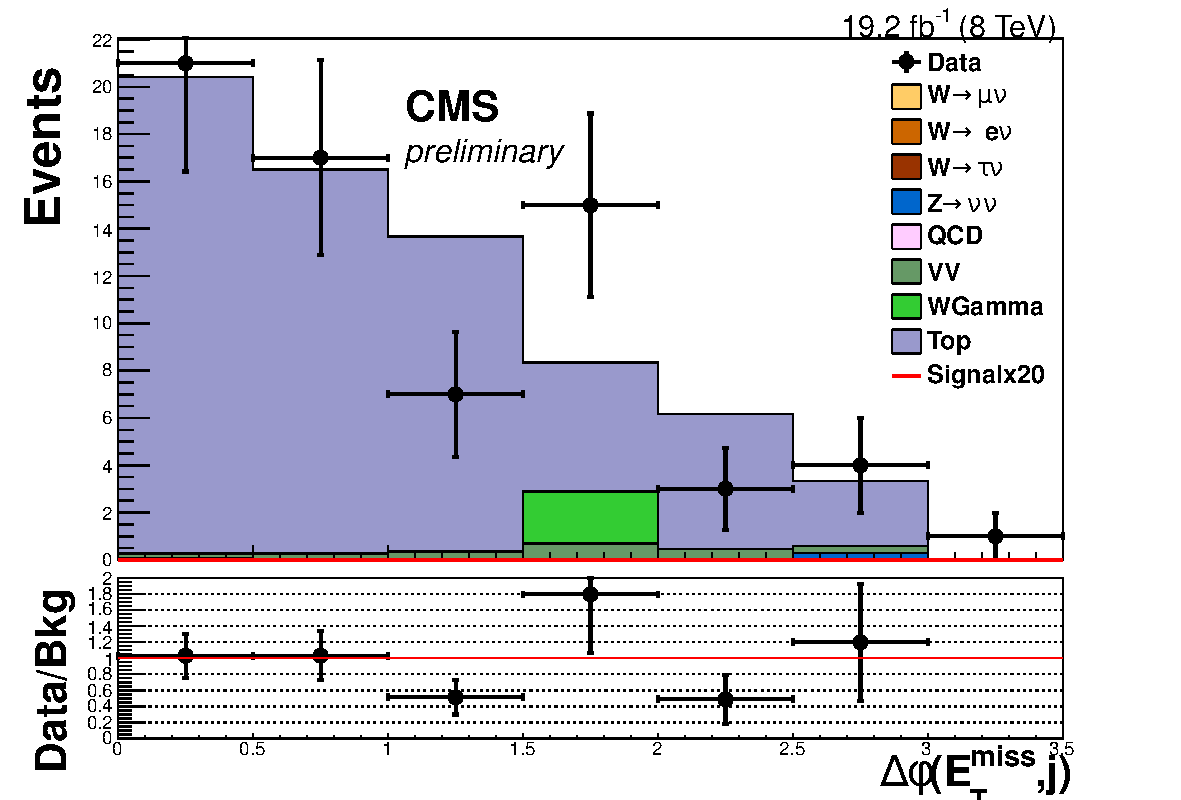
\includegraphics[width=.65\largefigwidth]{plots/parked/topjetmetdphicut0.pdf}}
  \subfloat[]{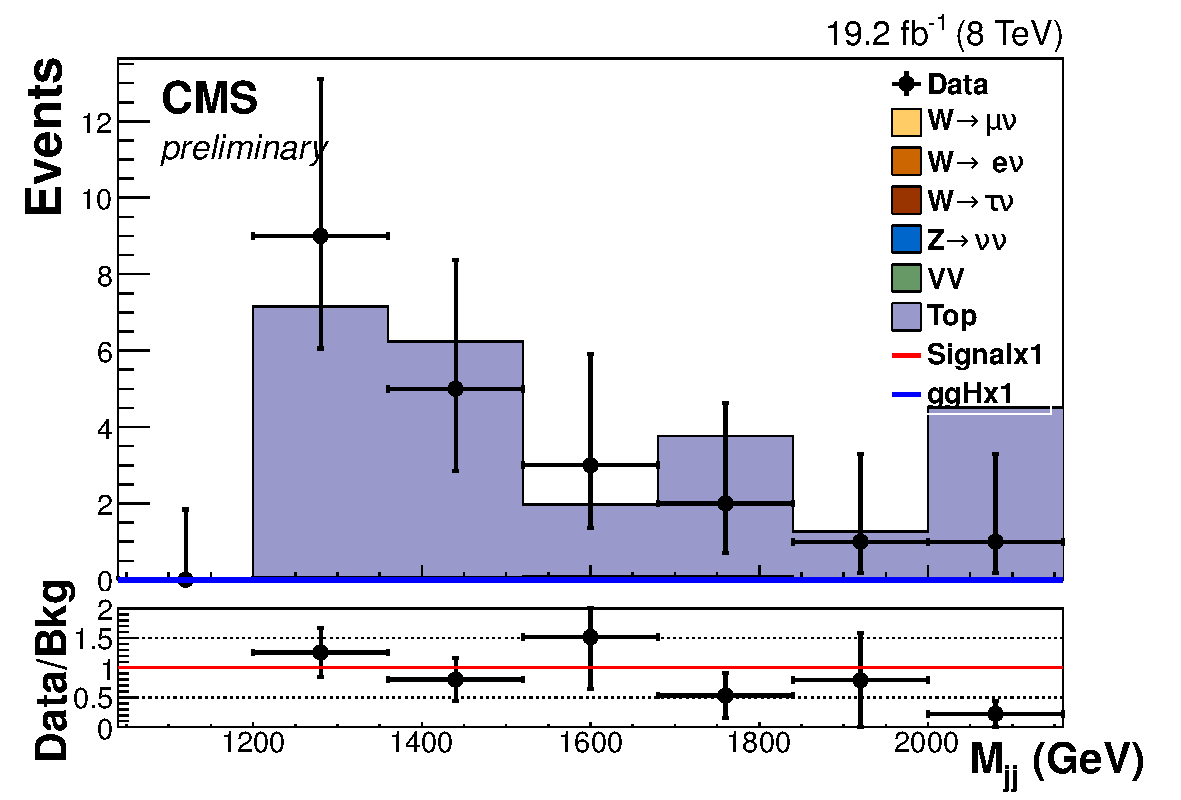
\includegraphics[width=.65\largefigwidth]{plots/parked/HIG-14-038-figs/output_sigreg/top_dijet_M.pdf}}
  \caption{The distribution of \jetmetdphi (a) and \Mjj (b) in the top control region with one tight electron and one tight muon. The last bin of each distribution contains the events above the range displayed.}
  \label{fig:parkedtopjetmetdphi}
\end{figure}


An issue with both of these control regions is that the ratio of pair production to single top quark production is very different from both the signal region and the $\PW\rightarrow\tau\nu$ control region. \ac{MC} estimations indicate that these top control regions have a negligible single top contribution, while the top background in the signal region has almost no top quark pair contribution. The $\PW\rightarrow\tau\nu$ region is expected to be a mixture, its top quark background being 30\% from single top events and 70\% for top quark pairs, again estimated from \ac{MC}. A single top control region was therefore also investigated.

The single top region differed from the signal region in that the \jetmetdphi cut was removed, exactly one tight electron or muon was required, further leptons were vetoed and one of the tag jets was required to be compatible with being a b-jet. The restriction to a single lepton significantly reduces the top quark pair production contribution where both resulting \PW bosons decay leptonically, and the requirement of one b-jet reduces the $\PW+$jets contribution. 

Identification of the b-jet was done using the \ac{CSV} discriminant~\cite{bjets}. B quarks are both heavier and longer lived than many other particles created at the \LHC, meaning that their secondary decay vertex can be distinguished from the \ac{PV}. \ac{CSV} is an \ac{MVA} based discriminant which uses information on secondary vertices and the lifetime of the particle to discriminate between jets from b quarks and those from light quarks. The medium working point used for this control region has an efficiency of approximately 85\% for b-quarks and mis-identifies light quark jets as b jets approximately 1\% of the time.

\ac{MC} estimates indicate the single top region is 17\% single top. This region again showed good data-\ac{MC} agreement (as can be seen in \FigureRef{fig:parkedsingletopjetmetdphi}) and a scale factor compatible with 1 within uncertainties. Because good agreement between data and \ac{MC} and scale factors compatible with 1 are seen in all investigated control regions, it was decided to use the \ac{MC} prediction for the top background in all regions with no additional scale factor. A 20\% systematic uncertainty was applied to this prediction which covered the largest deviation from 1 seen in the scale factors from the various control regions.

\begin{figure}
  \subfloat[]{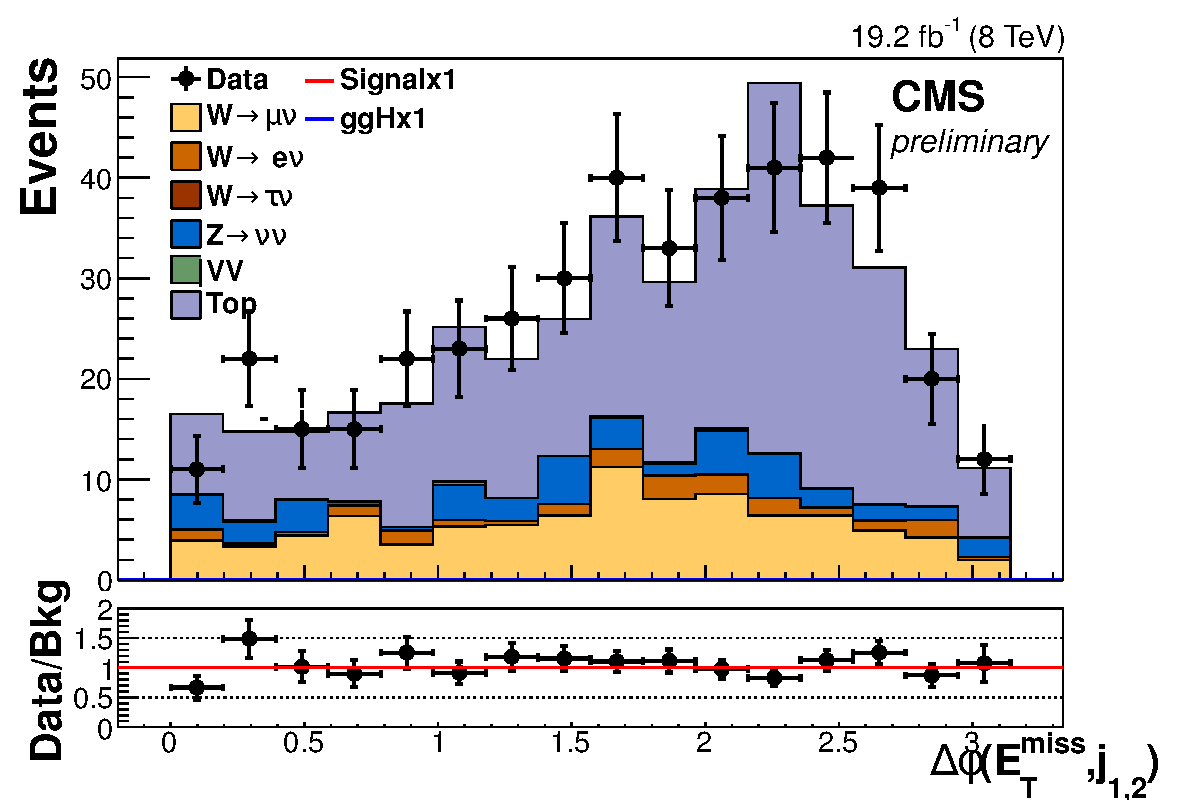
\includegraphics[width=.65\largefigwidth]{plots/parked/output_singletop/top_jetmetnomu_mindphi.pdf}}
  \subfloat[]{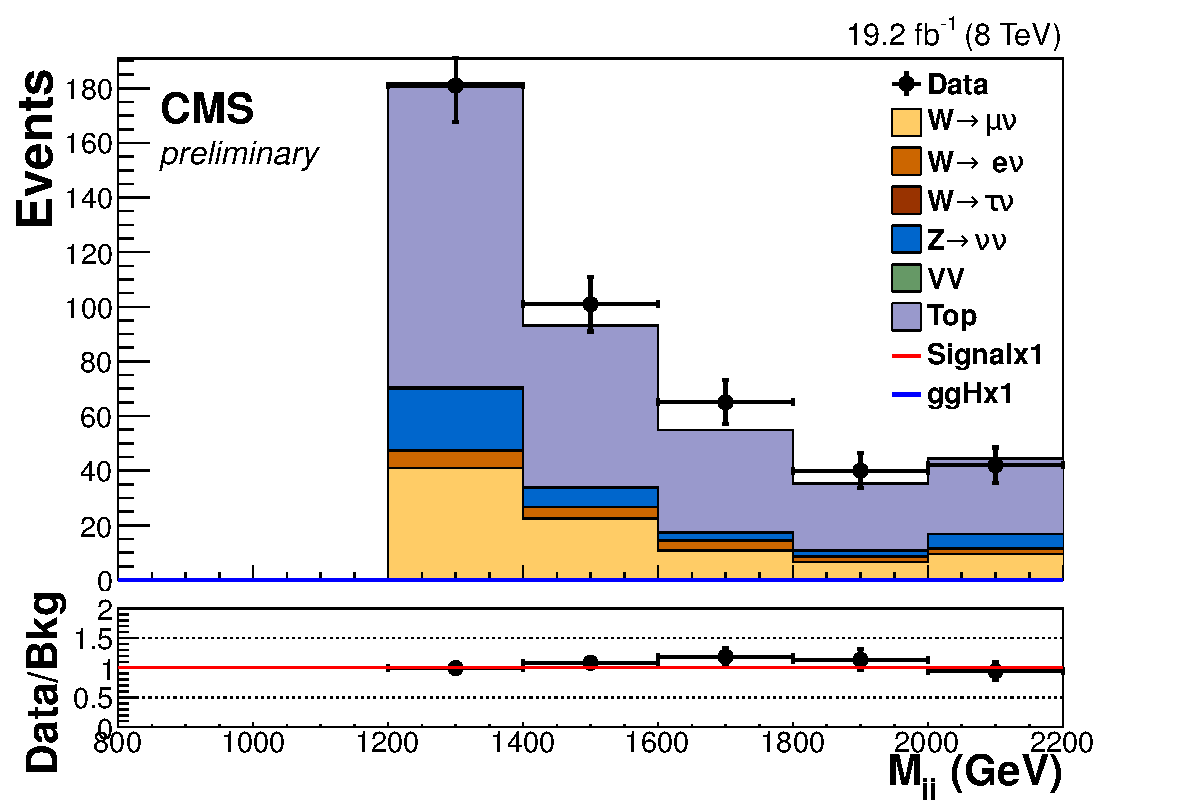
\includegraphics[width=.65\largefigwidth]{plots/parked/output_singletop/top_dijet_M.pdf}}
  \caption{The distribution of \jetmetdphileading (a) and \Mjj (b) in the single top control region. The last bin of each distribution contains the events above the range displayed.}
  \label{fig:parkedsingletopjetmetdphi}
\end{figure}

\subsection{W$\rightarrow e\nu$+jets}
\label{sec:parkedwenu}
The $\PW\rightarrow e\nu$ background in the parked data analysis is estimated using the same method as that used for the prompt analysis based on \EquationRef{eq:wdatabkgrep}. The control region used has the same requirements as the signal region, except that the electron veto is replaced with a requirement that there is one tight electron and no other electrons present in the event. The requirement of an electron removes signal events and enriches the region in $\PW\rightarrow e\nu$ events. The distributions of several variables in data and \ac{MC} (which has been scaled by the data driven scale factor extracted from this control region) are shown in \FigureRef{fig:parkedwenu}, where good agreement can be seen. A table of the inputs to, and results of, \EquationRef{eq:wdatabkgrep} can be seen in \TableRef{tab:parkedwenu}. The table also shows that the expected contribution to this region from other background processes is small, being approximately 5\%. The scale factor obtained for this background is 0.5, which is significantly different from 1, this difference is further investigated in \SectionRef{sec:parkedscalefactors}.

\begin{table}
  \begin{center}
    \caption{The inputs to, and results of, \EquationRef{eq:wdatabkgrep}, when used to estimate the $W\rightarrow e\nu$ estimate in the signal
      region.}
    \label{tab:parkedwenu}
    \begin{tabular}{lcc}
      \hline
      \hline
      & Signal region & Control region \\
      \hline
      \hline
      $N_{Data}$&N/A&$68\pm 8.2$\stat\\
      $N_{Bkg}$&N/A&$3.5\pm 1.2(\rm{MC\,stat})$\\
      $N_{MC}$&$114.9\pm8.9(\rm{MC\,stat})$&$128.0\pm 8.0(\rm{MC\,stat})$\\
      \hline
      $\frac{N^{data}-N^{bkg}}{N^{W MC}_{C}}$ & \multicolumn{2}{c|}{$0.50\pm0.06$\stat$\pm0.03$(MC stat)} \\
      \hline
      $N_{\PW\rightarrow e\nu}$&\textcolor{red}{$57.9\pm7.4$\stat$\pm7.7$\syst}&N/A \\
        \hline
        \hline
    \end{tabular}
  \end{center}
\end{table}

\begin{figure}
  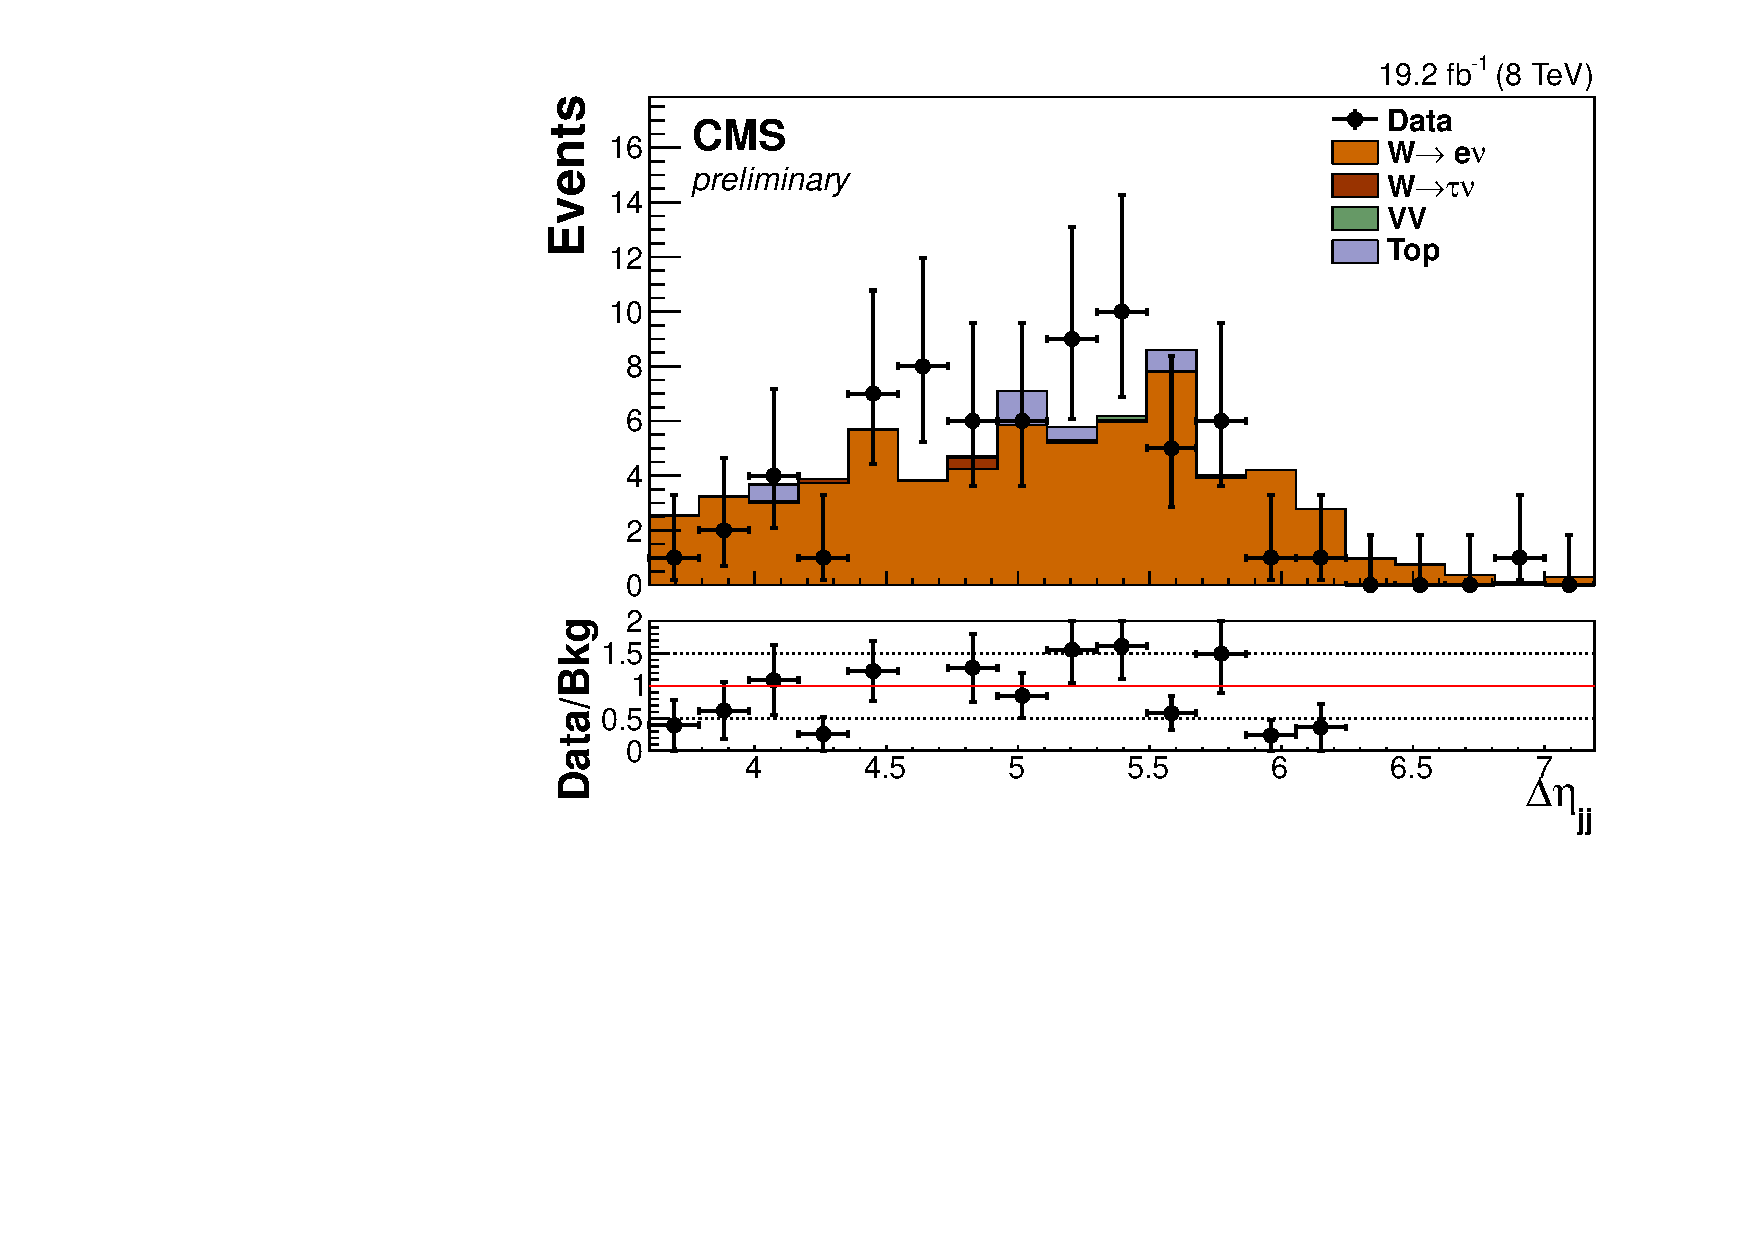
\includegraphics[width=.65\largefigwidth]{plots/parked/HIG-14-038-figs/output_sigreg/enu_dijet_deta.pdf}
  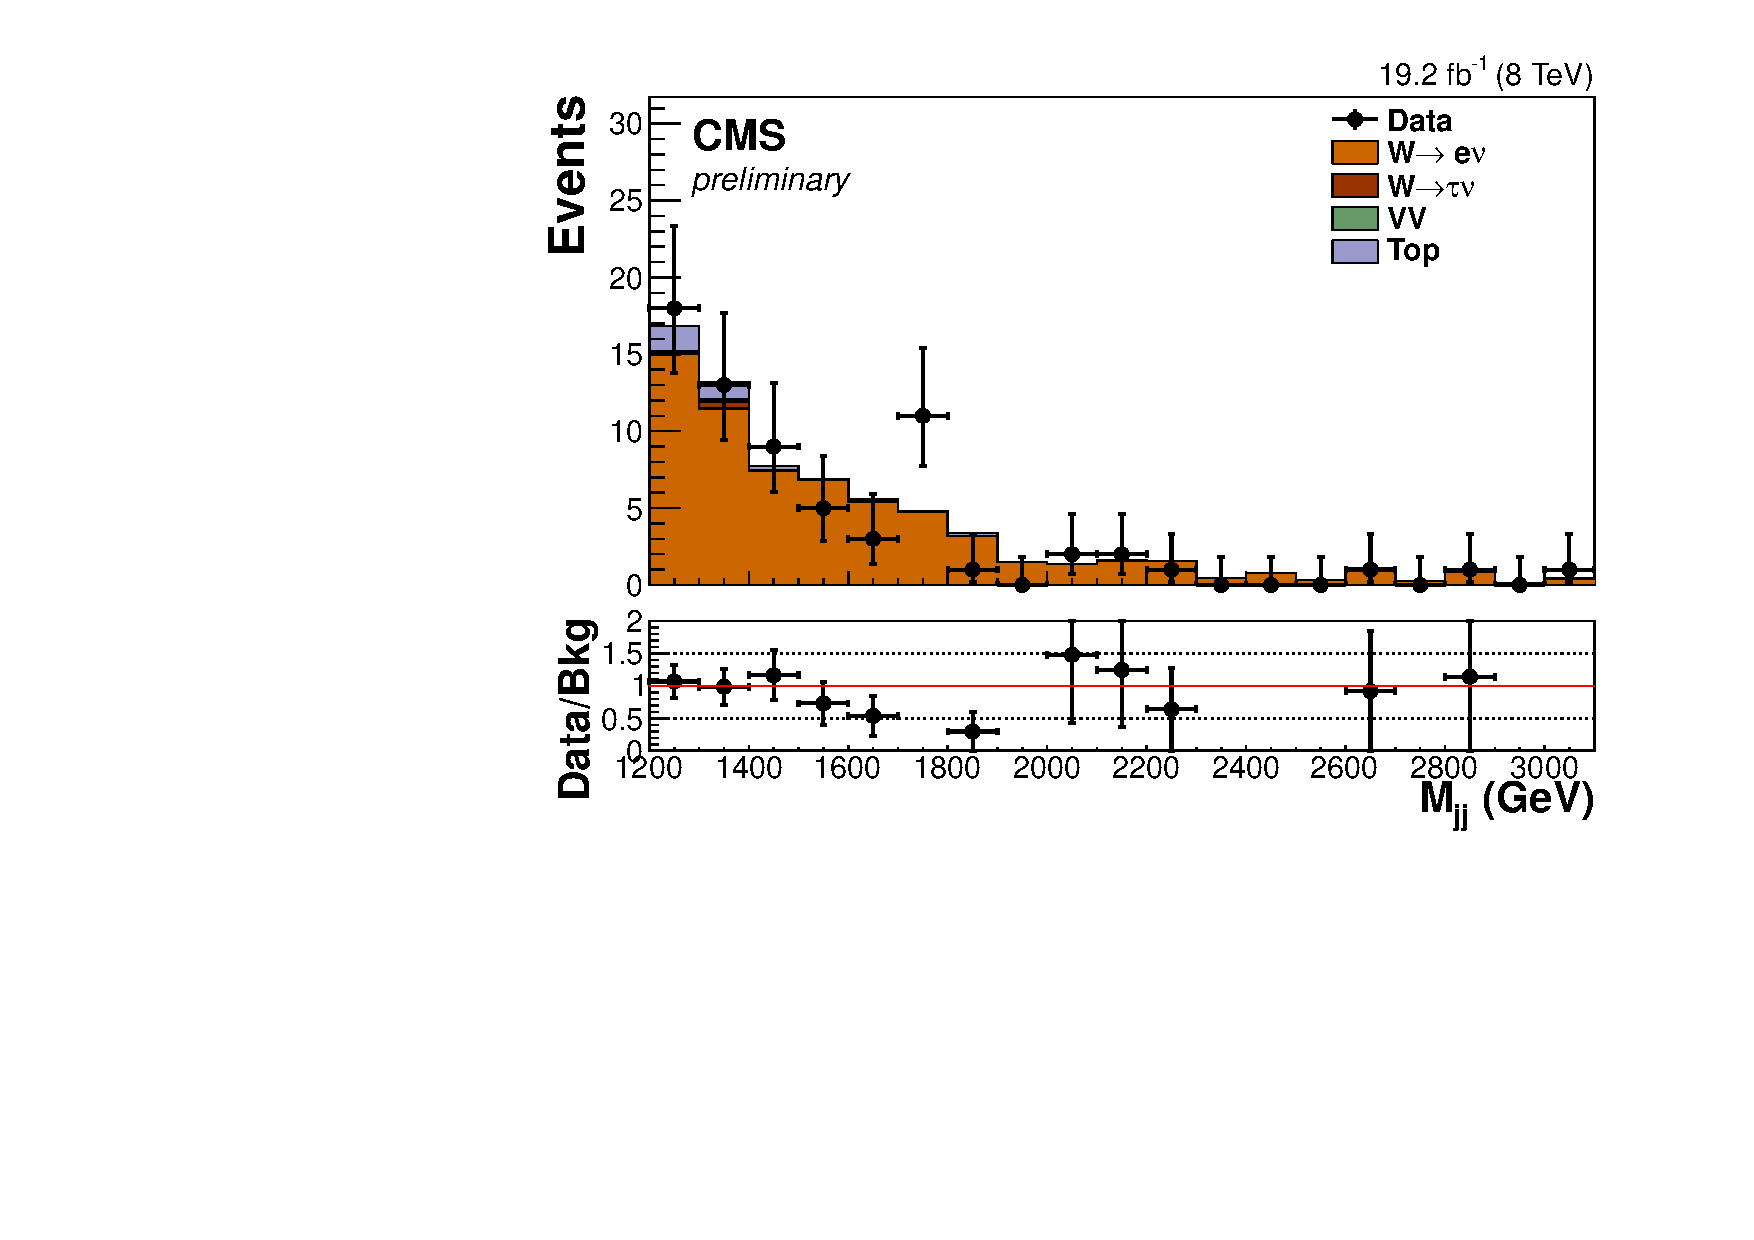
\includegraphics[width=.65\largefigwidth]{plots/parked/HIG-14-038-figs/output_sigreg/enu_dijet_M.pdf}

  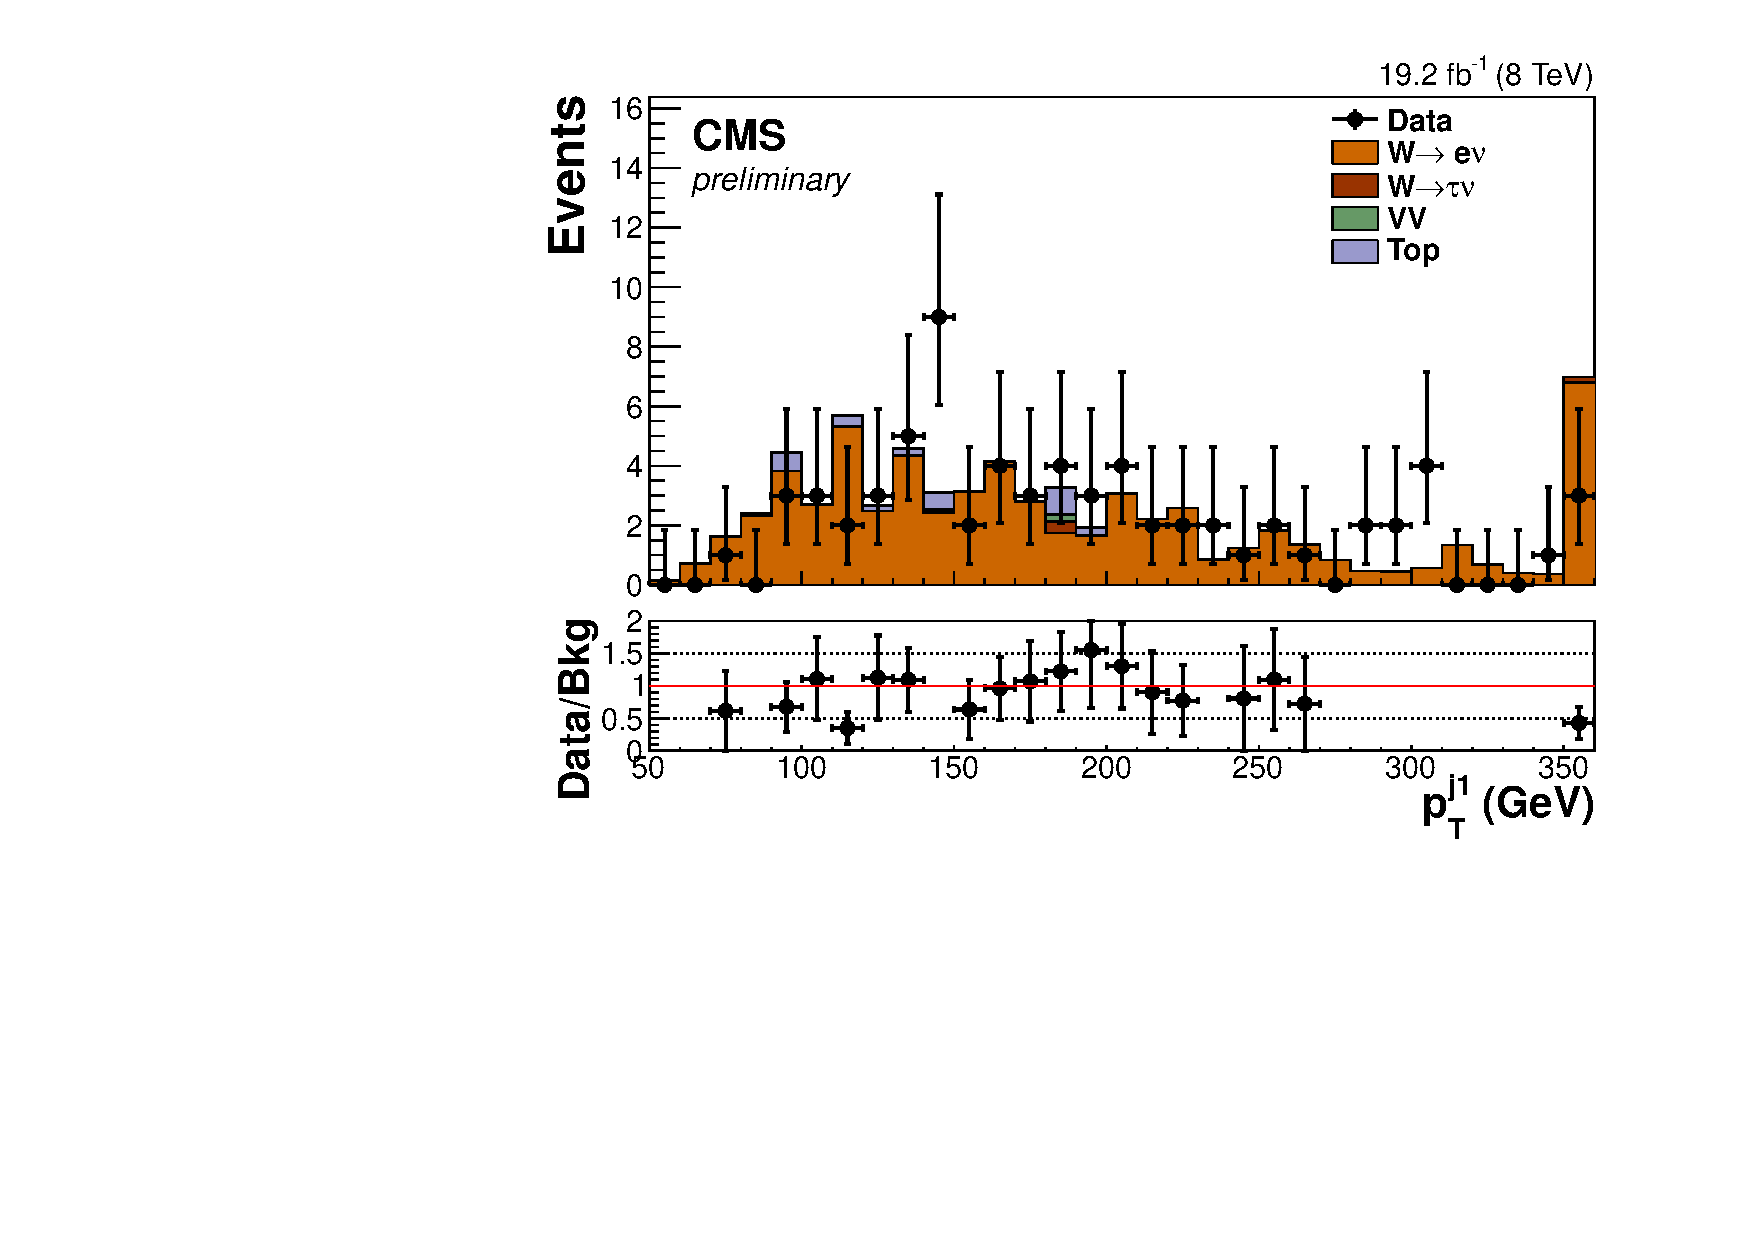
\includegraphics[width=.65\largefigwidth]{plots/parked/HIG-14-038-figs/output_sigreg/enu_jet1_pt.pdf}
  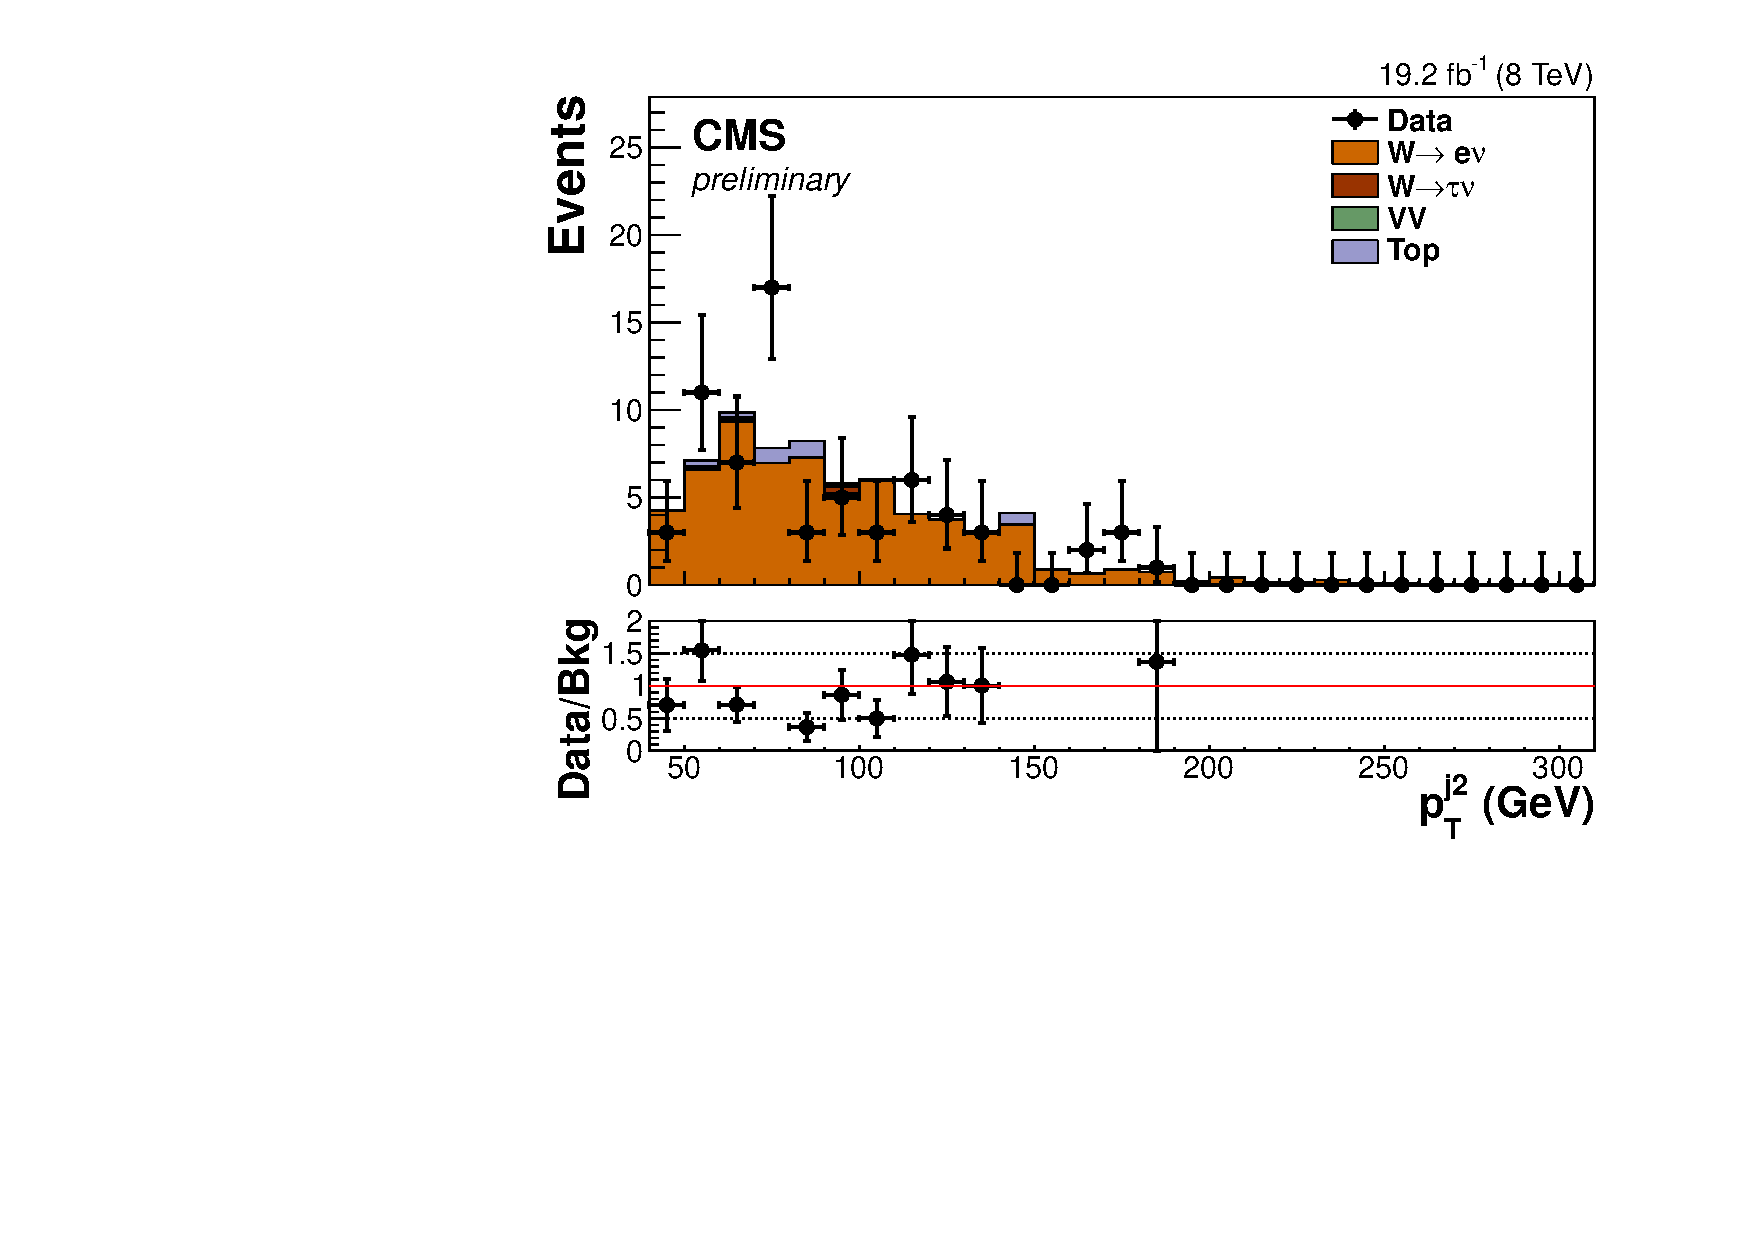
\includegraphics[width=.65\largefigwidth]{plots/parked/HIG-14-038-figs/output_sigreg/enu_jet2_pt.pdf}

  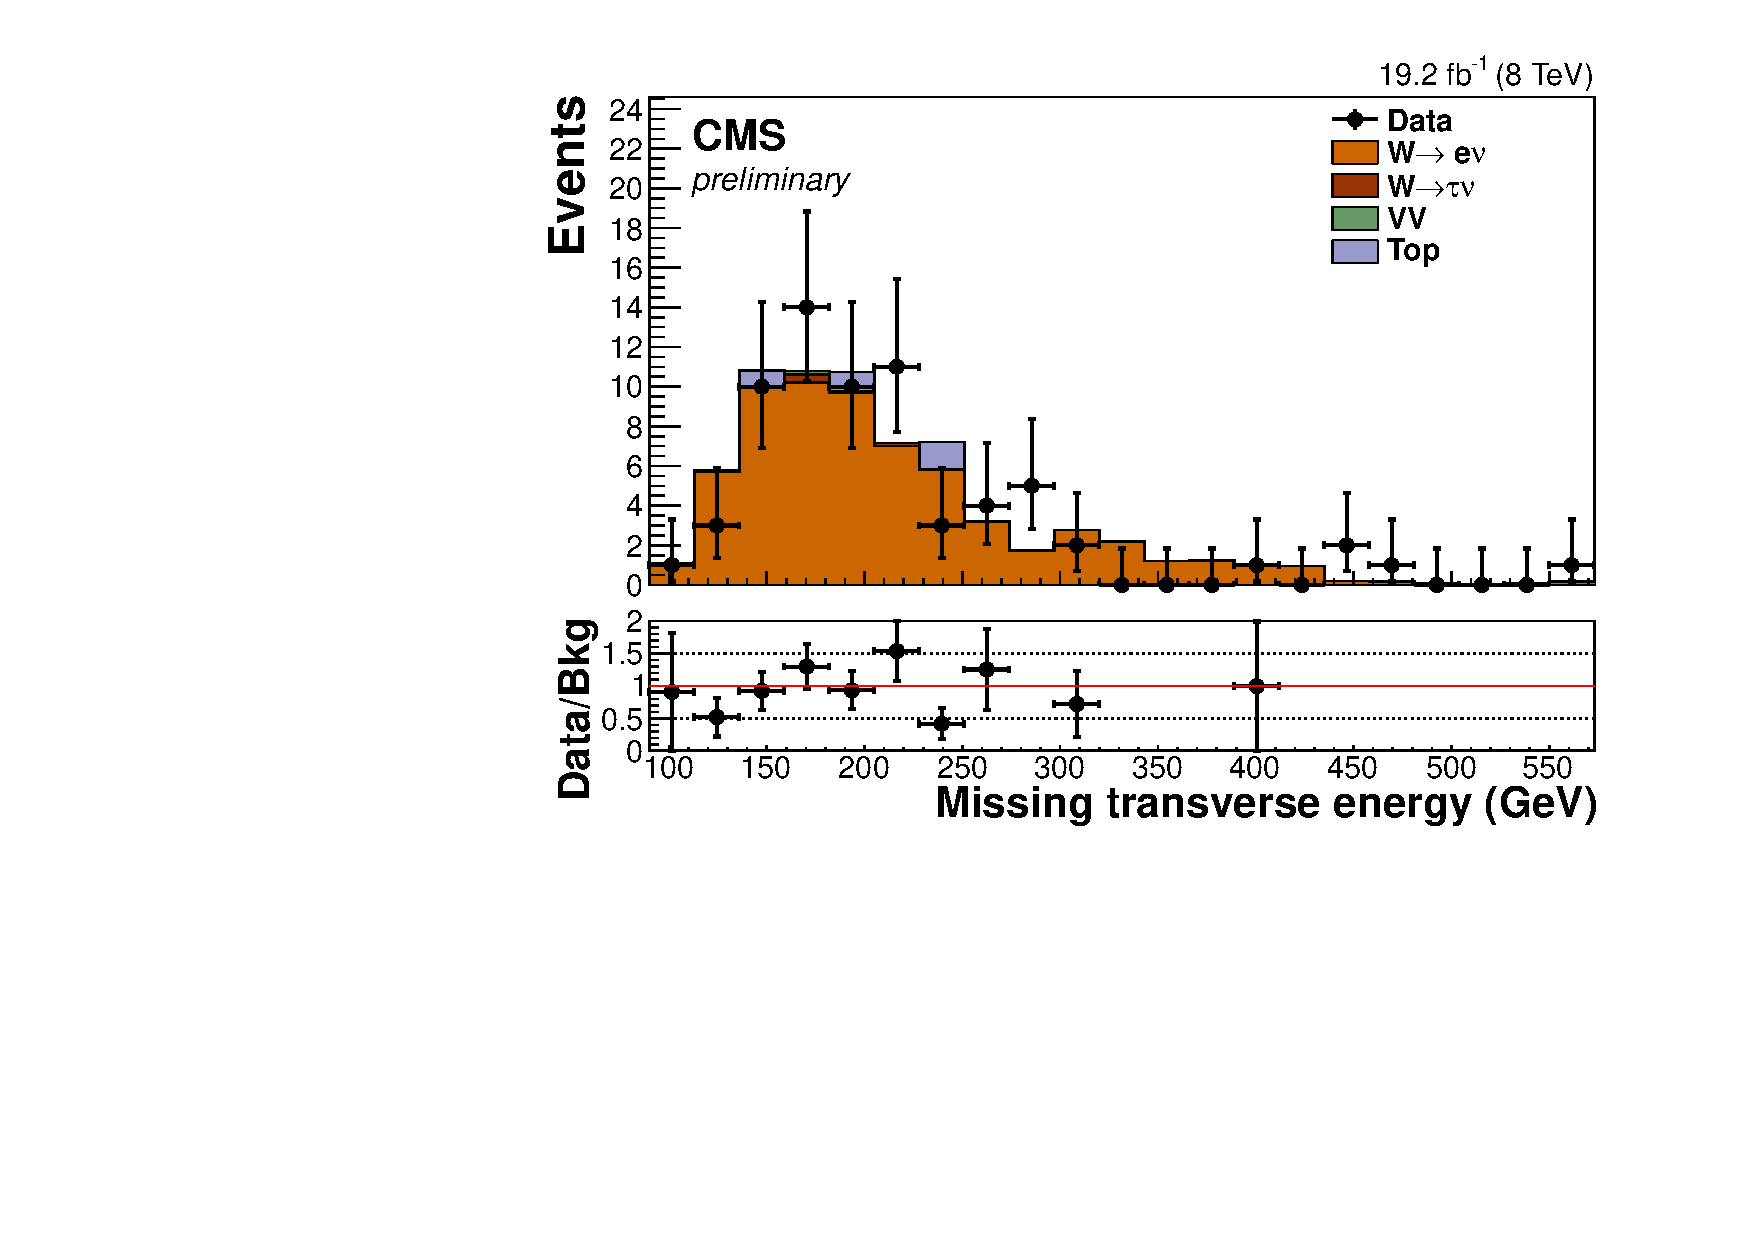
\includegraphics[width=.65\largefigwidth]{plots/parked/HIG-14-038-figs/output_sigreg/enu_metnomuons.pdf}
  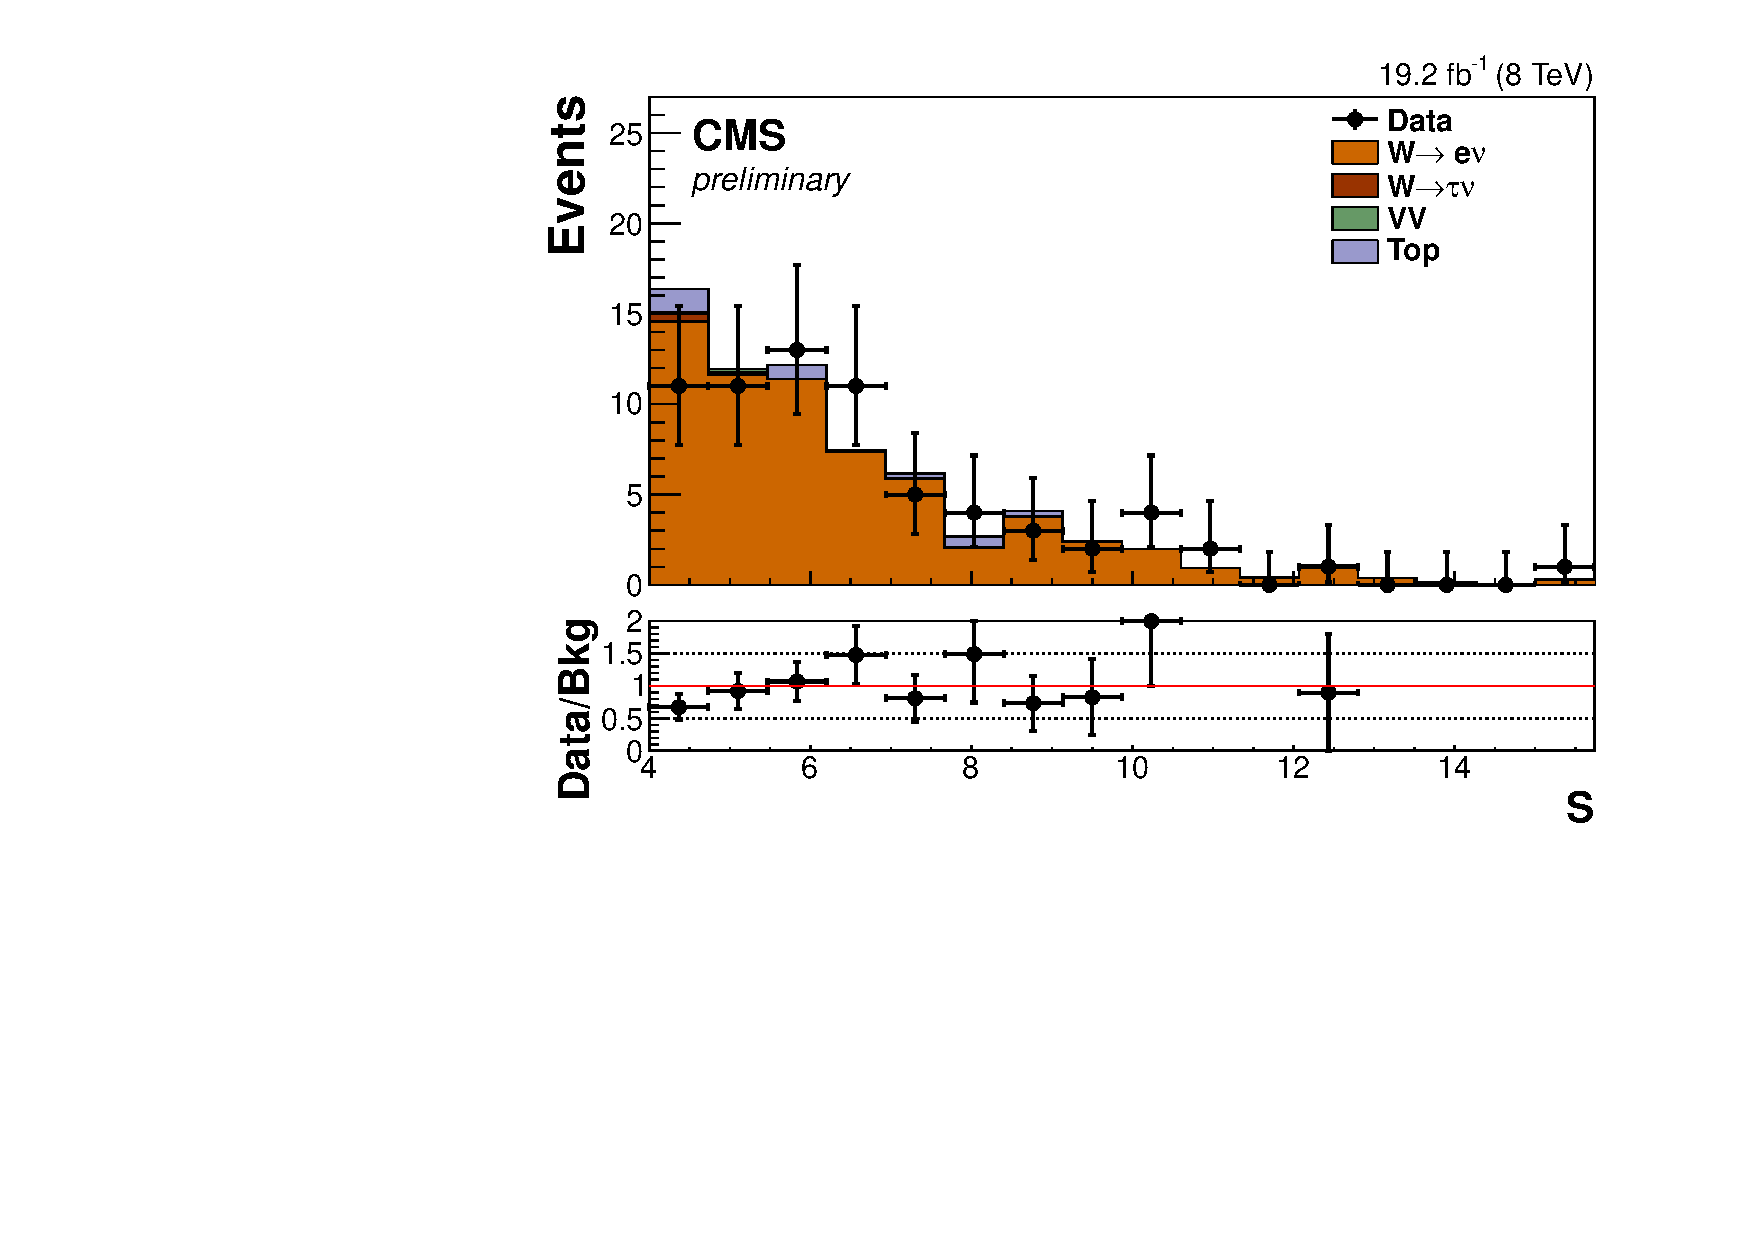
\includegraphics[width=.65\largefigwidth]{plots/parked/HIG-14-038-figs/output_sigreg/enu_metnomu_significance.pdf}
  
  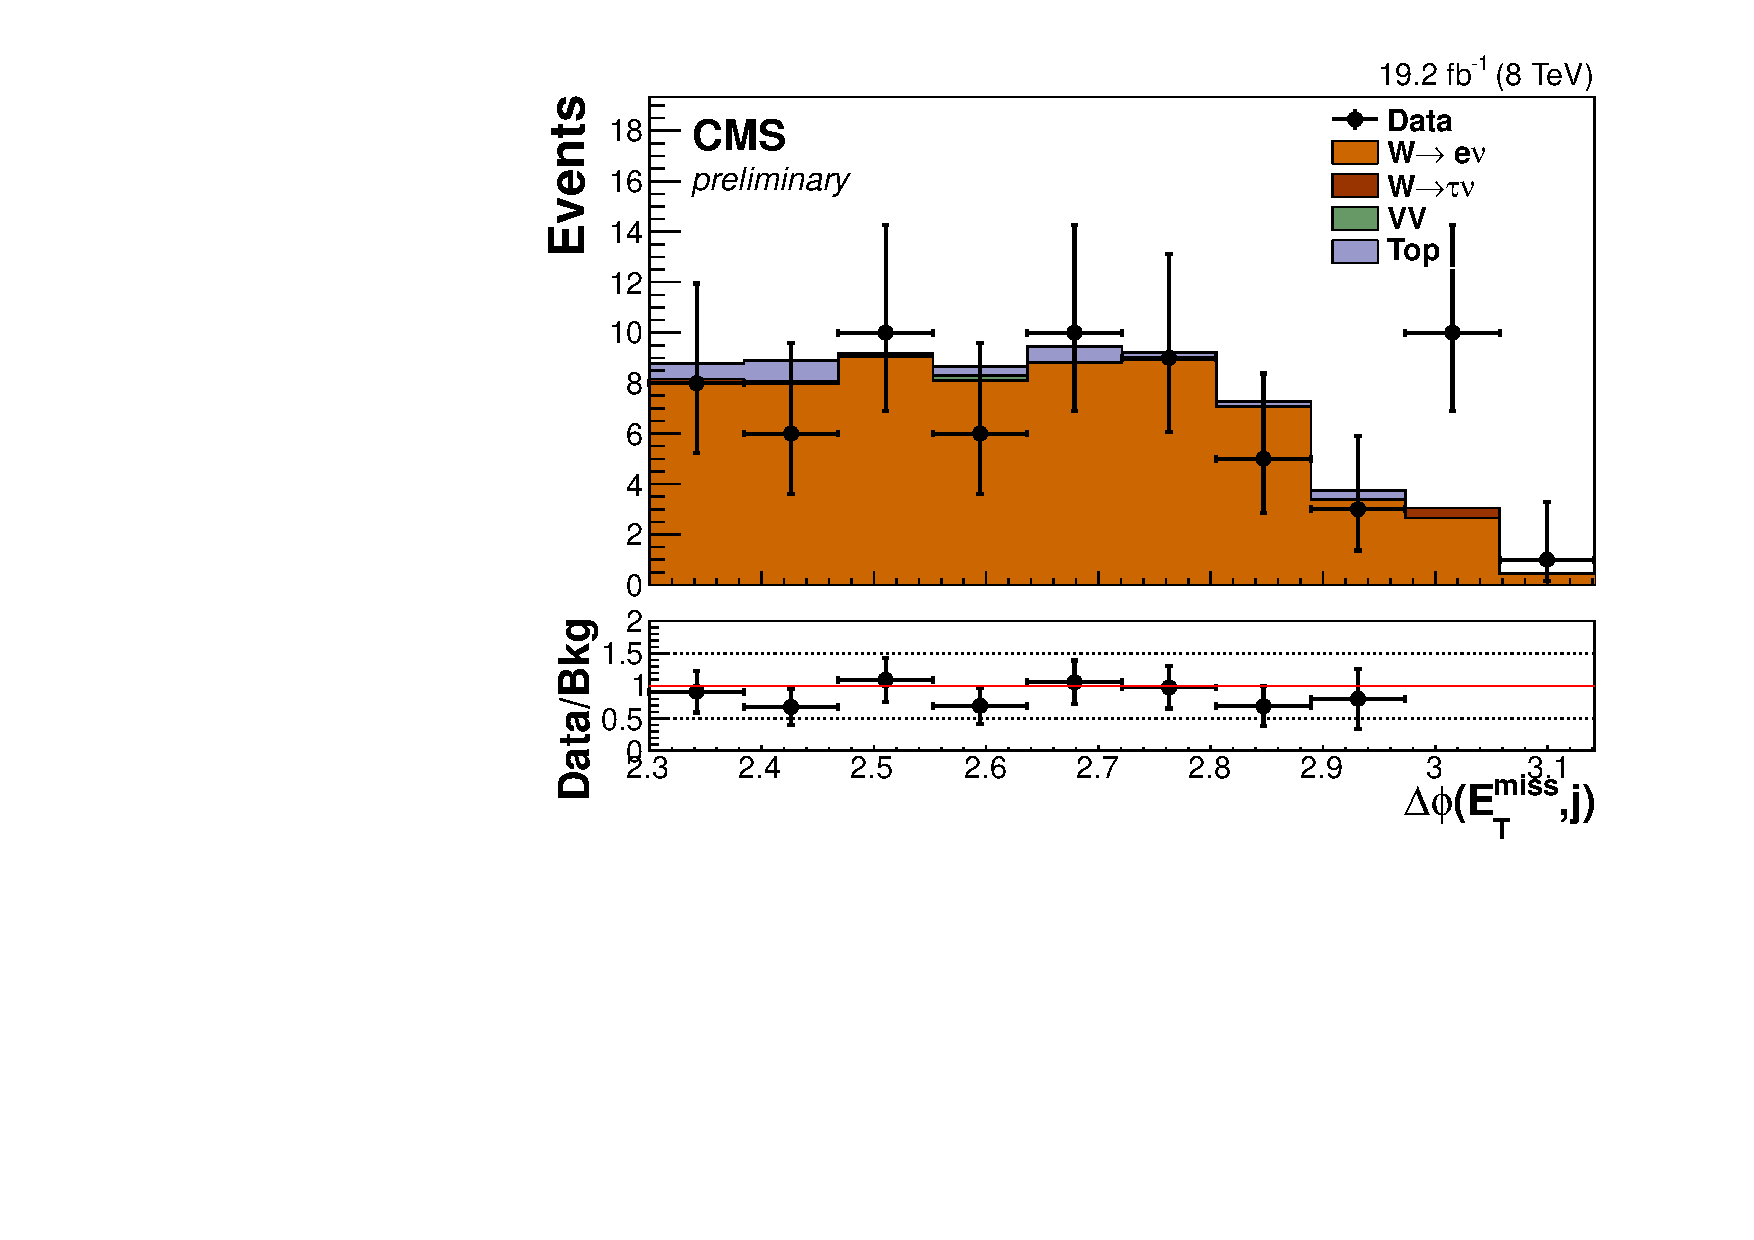
\includegraphics[width=.65\largefigwidth]{plots/parked/HIG-14-038-figs/output_sigreg/enu_alljetsmetnomu_mindphi.pdf}

  \caption{Distributions of variables in data and \ac{MC} events in the $\PW\rightarrow e\nu$ control region. \ac{MC} events from V+jets backgrounds are scaled by their data-driven scale factors. The variables shown are from top to bottom and left to right \detajj, \Mjj, the leading and sub-leading jet's \pt, \METnoMU, \METsig and \jetmetdphi. The last bin of each distribution contains the events above the range displayed~\cite{CMS-PAS-HIG-14-038}.}
  \label{fig:parkedwenu}
\end{figure}

\subsection{W$\rightarrow \mu\nu$+jets}
\label{sec:parkedwmunu}
As for the $\PW\rightarrow e\nu$ background the $W\rightarrow \mu\nu$ background is estimated using \EquationRef{eq:wdatabkgrep} with a control region enriched in $\PW\rightarrow\mu\nu$ events through a change in lepton requirements. The control region used has the same requirements as the signal region, but with the muon veto replaced with a requirement that there is one tight muon and no other muons present in the event. The distributions of several variables in data and \ac{MC} (which has been scaled by the data driven scale factor extracted from this control region) are shown in \FigureRef{fig:parkedwmunu}, where good agreement can be seen. A table of the inputs to, and results of, \EquationRef{eq:wdatabkgrep} can be seen in \TableRef{tab:parkedwmunu}. The contribution from other backgrounds in the $\PW\rightarrow\mu\nu$ control region is approximately 5\%. Again the scale factor obtained  for this background is significantly different from 1, being 0.71, and further investigation of this is detailed in \SectionRef{sec:parkedscalefactors}. Furthermore, the estimated contribution from this background is very different to that expected from $\PW\rightarrow e\nu$, an investigation of this difference is described in \SectionRef{sec:parkedenumunudiff}.

\begin{figure}
  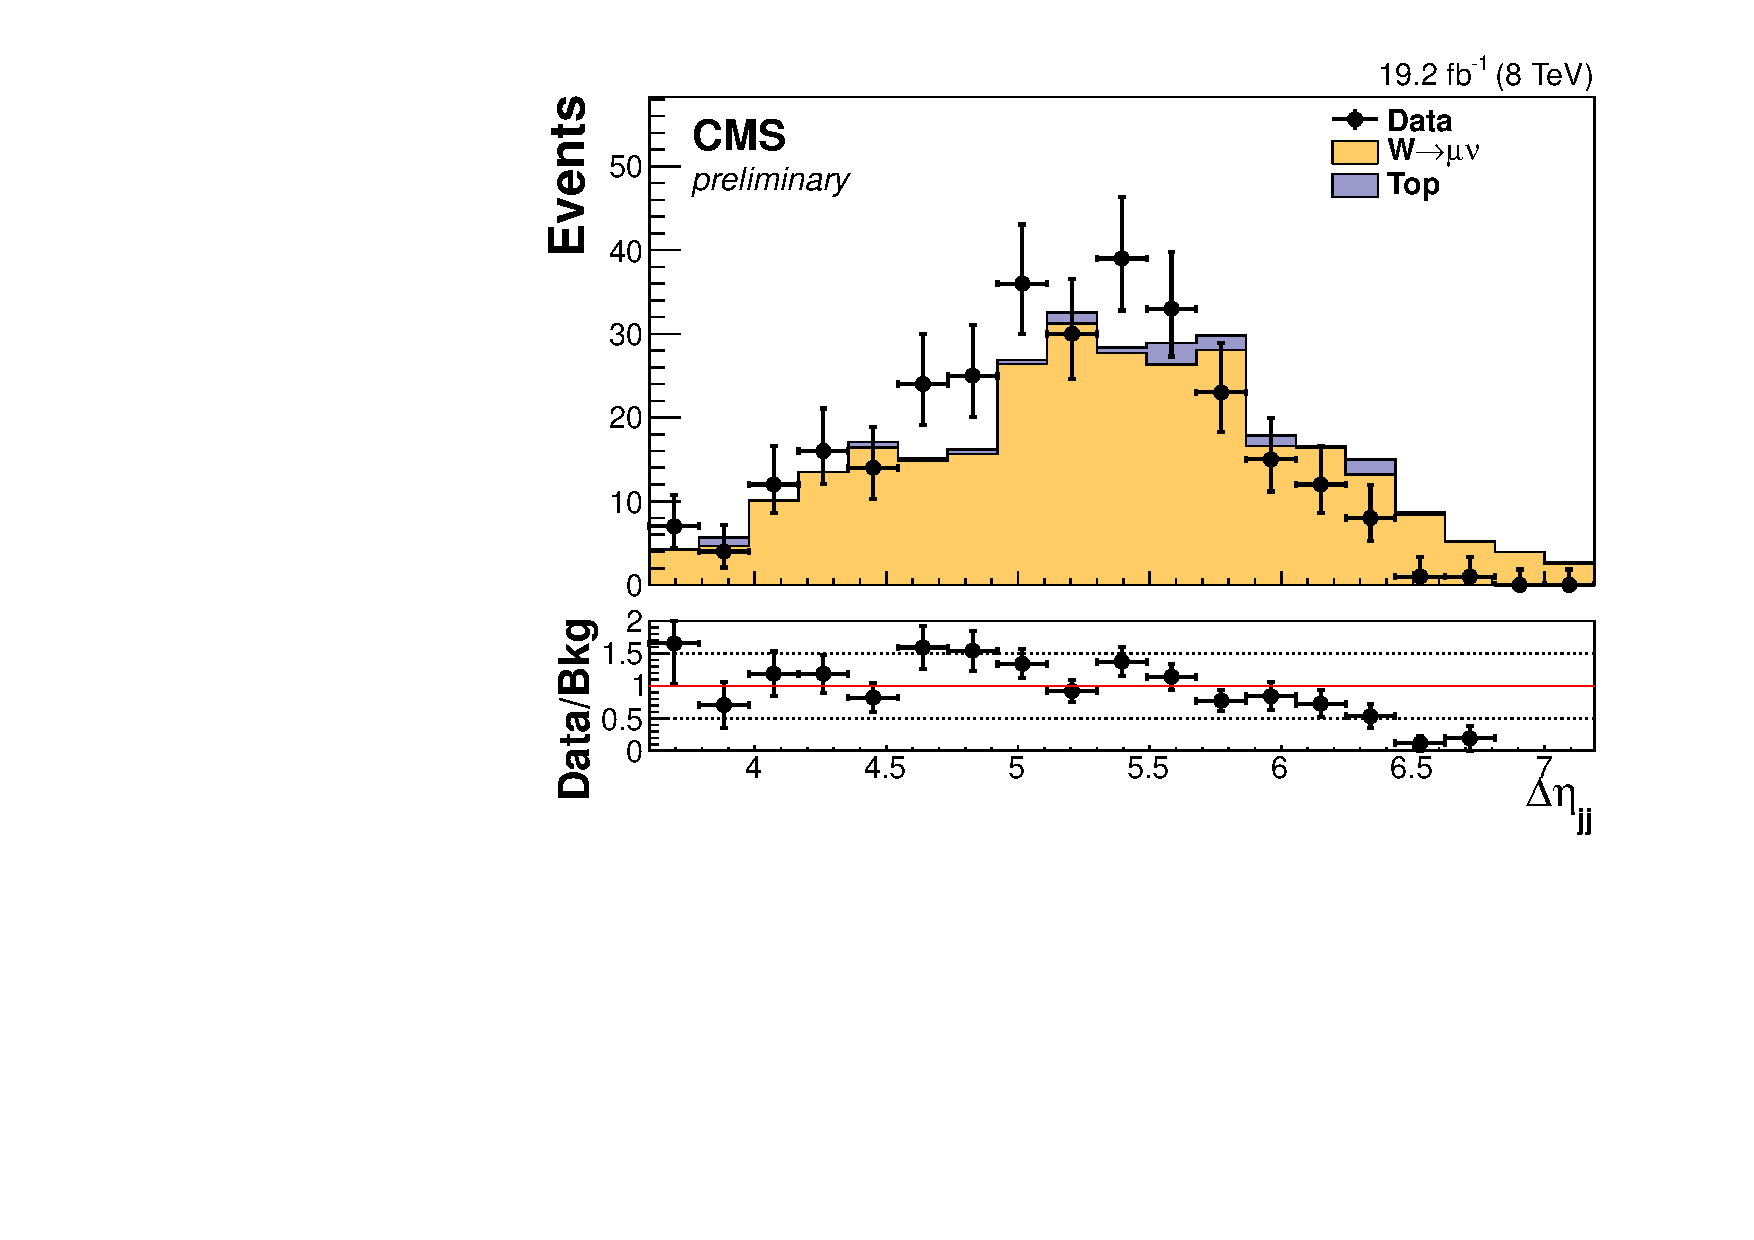
\includegraphics[width=.65\largefigwidth]{plots/parked/HIG-14-038-figs/output_sigreg/munu_dijet_deta.pdf}
  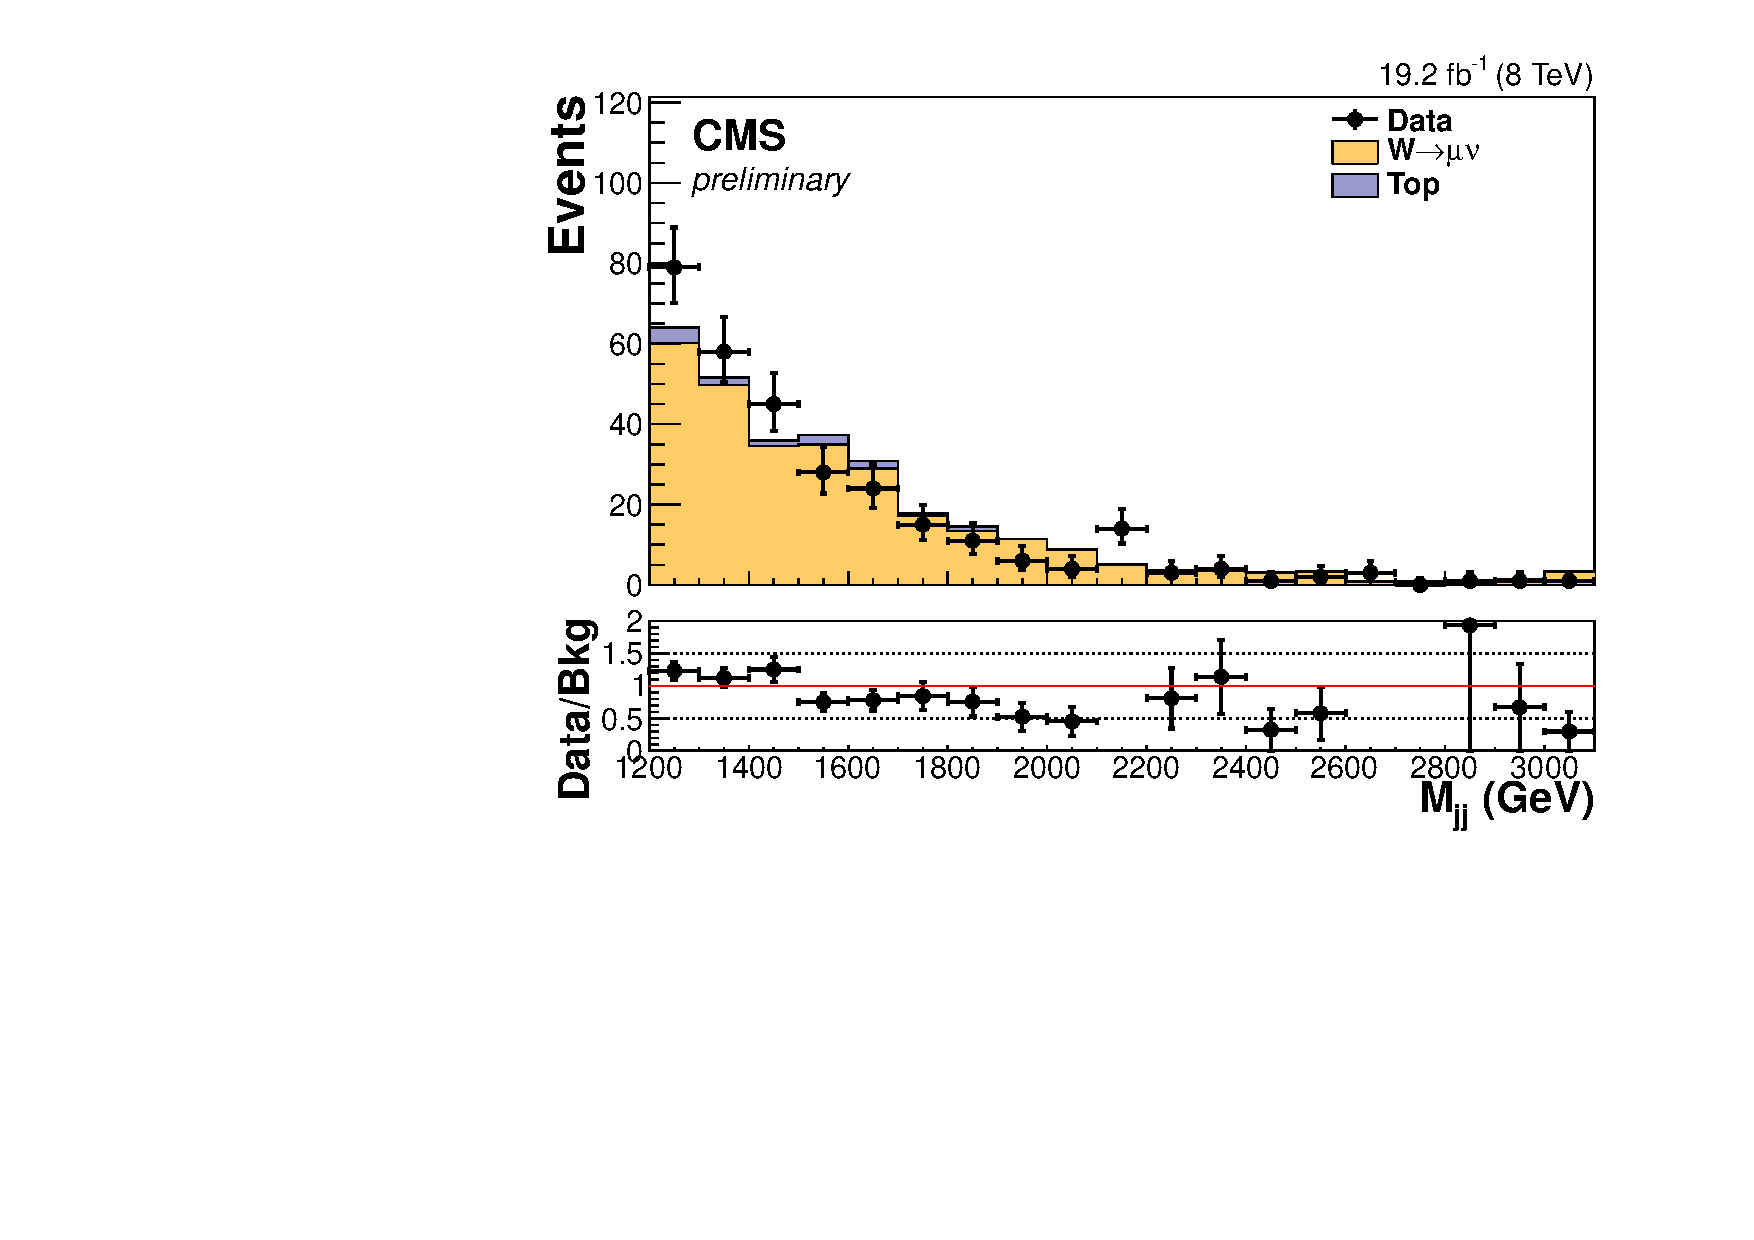
\includegraphics[width=.65\largefigwidth]{plots/parked/HIG-14-038-figs/output_sigreg/munu_dijet_M.pdf}

  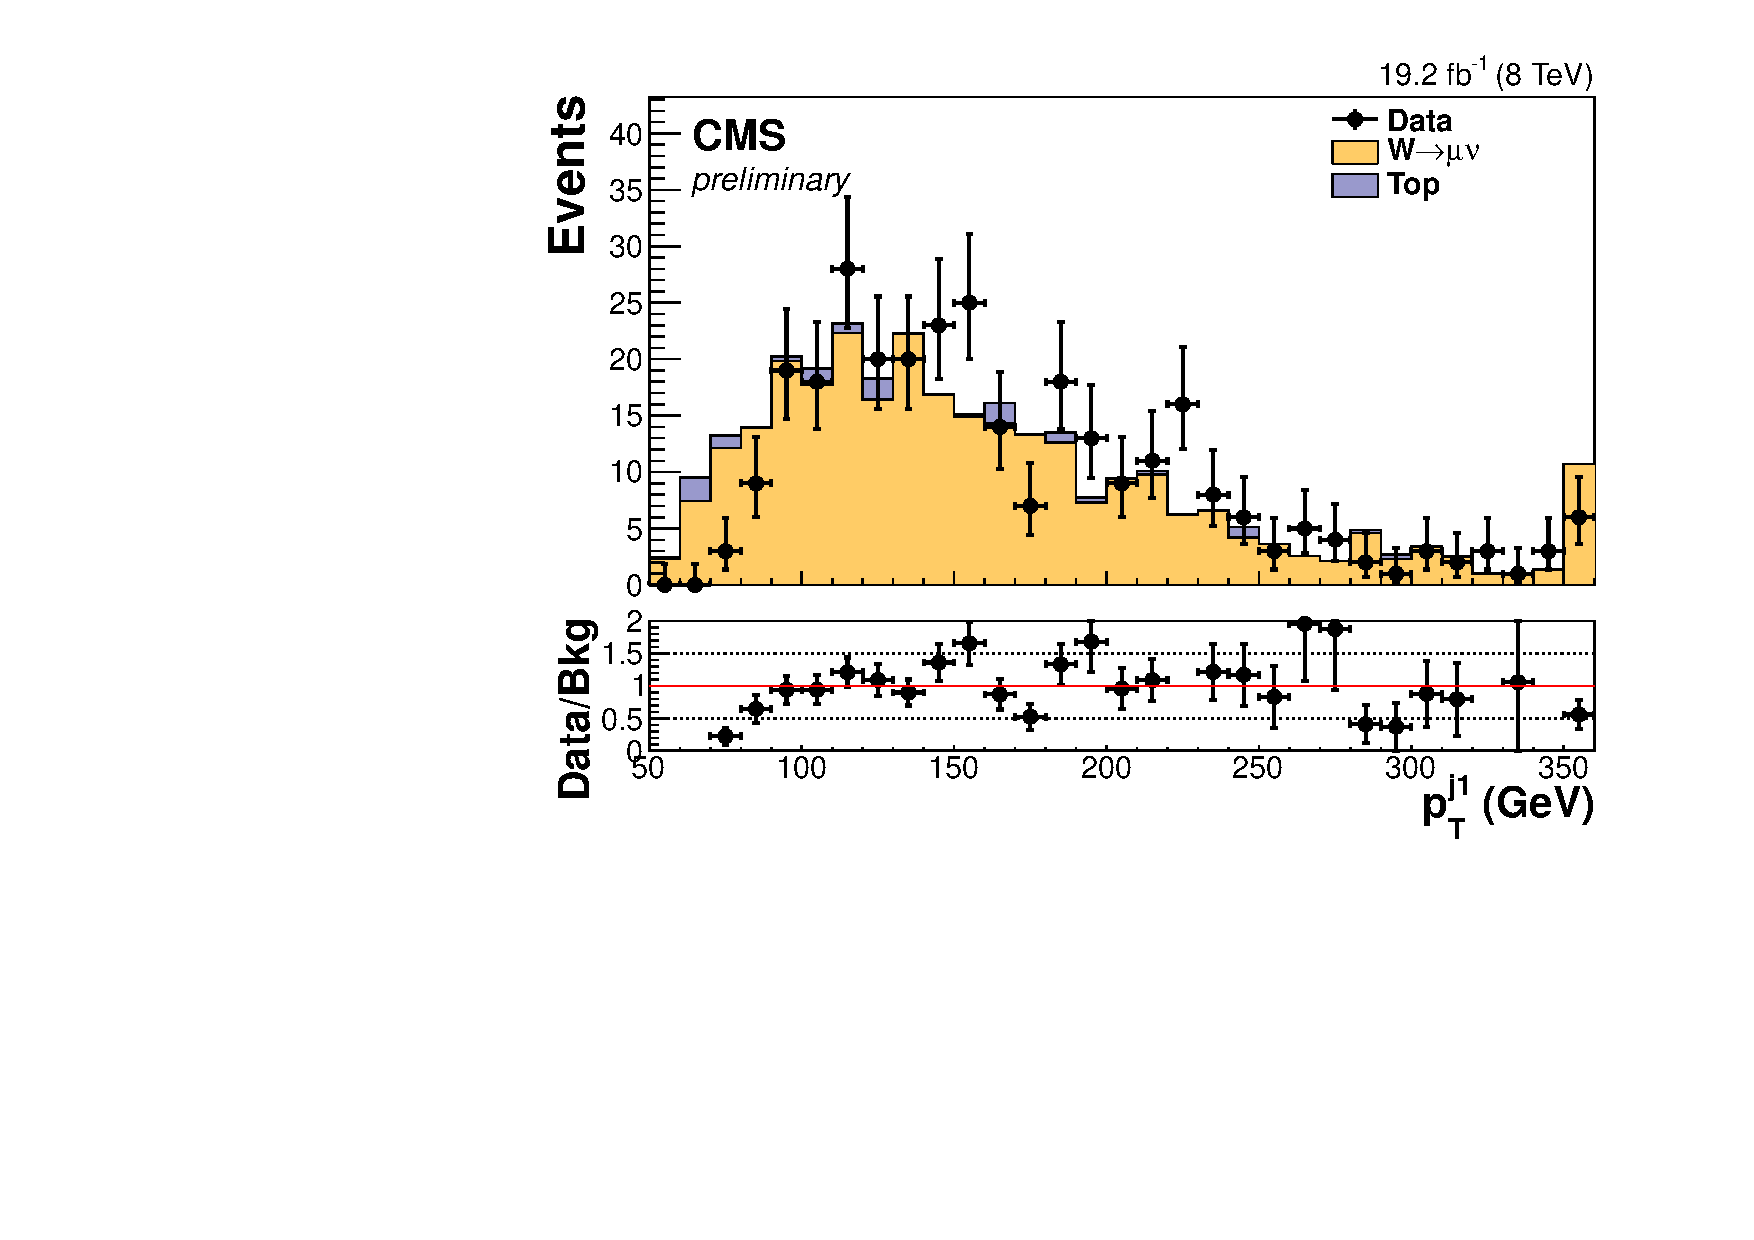
\includegraphics[width=.65\largefigwidth]{plots/parked/HIG-14-038-figs/output_sigreg/munu_jet1_pt.pdf}
  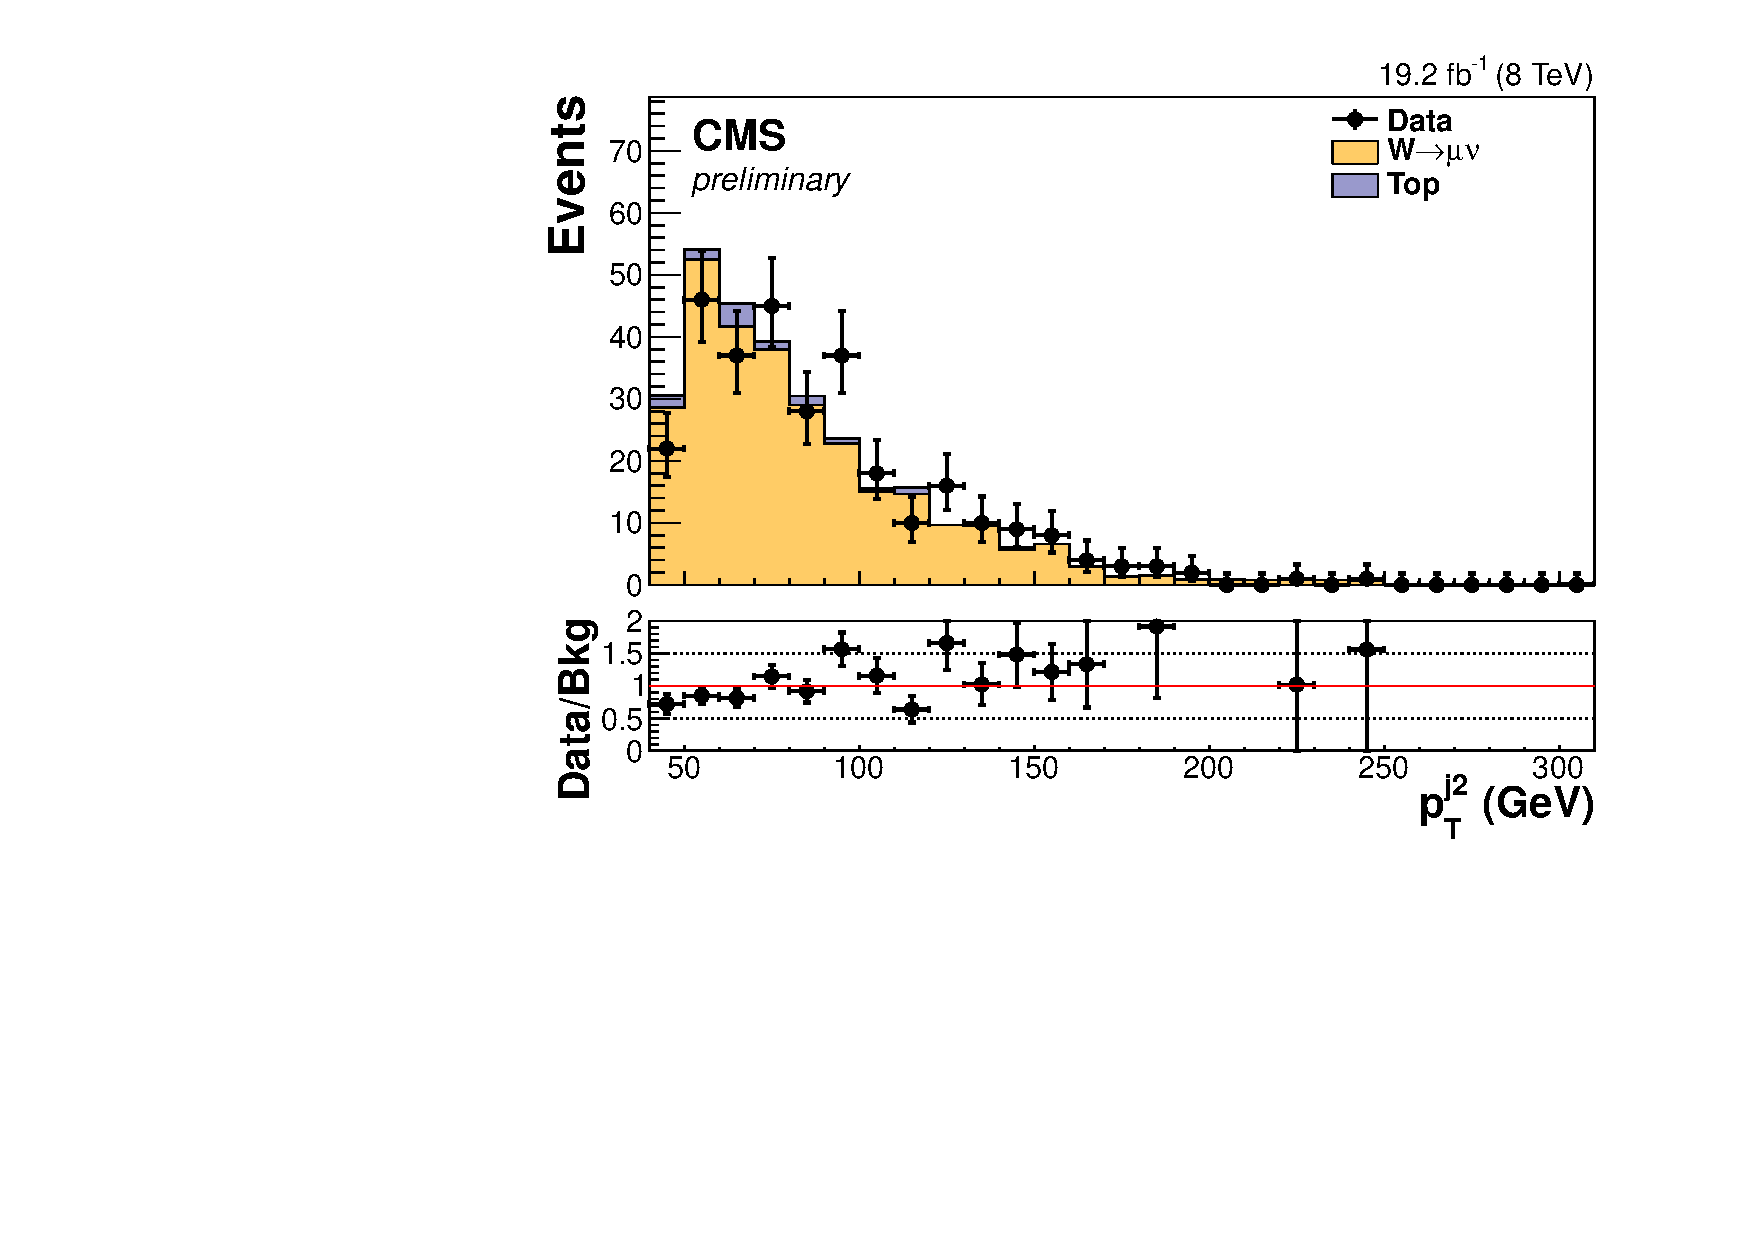
\includegraphics[width=.65\largefigwidth]{plots/parked/HIG-14-038-figs/output_sigreg/munu_jet2_pt.pdf}

  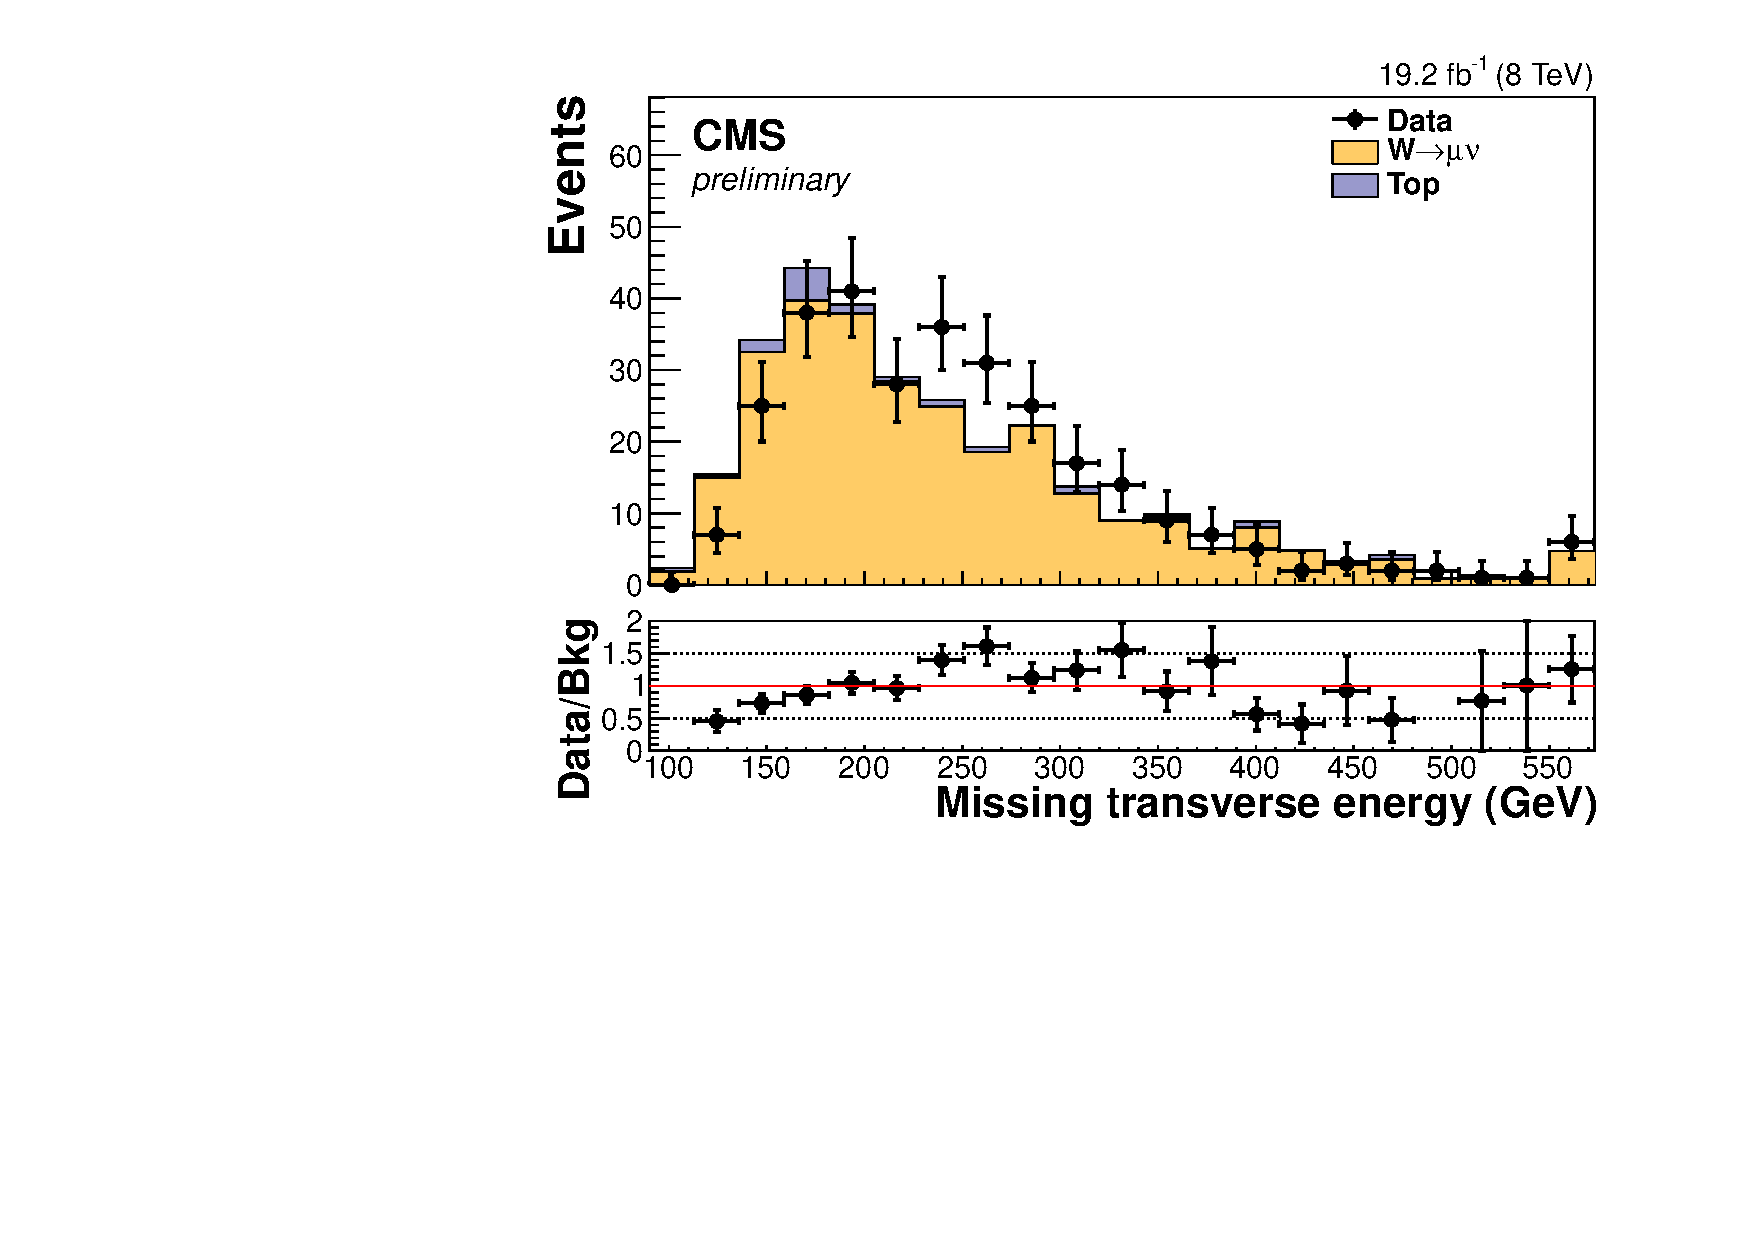
\includegraphics[width=.65\largefigwidth]{plots/parked/HIG-14-038-figs/output_sigreg/munu_metnomuons.pdf}
  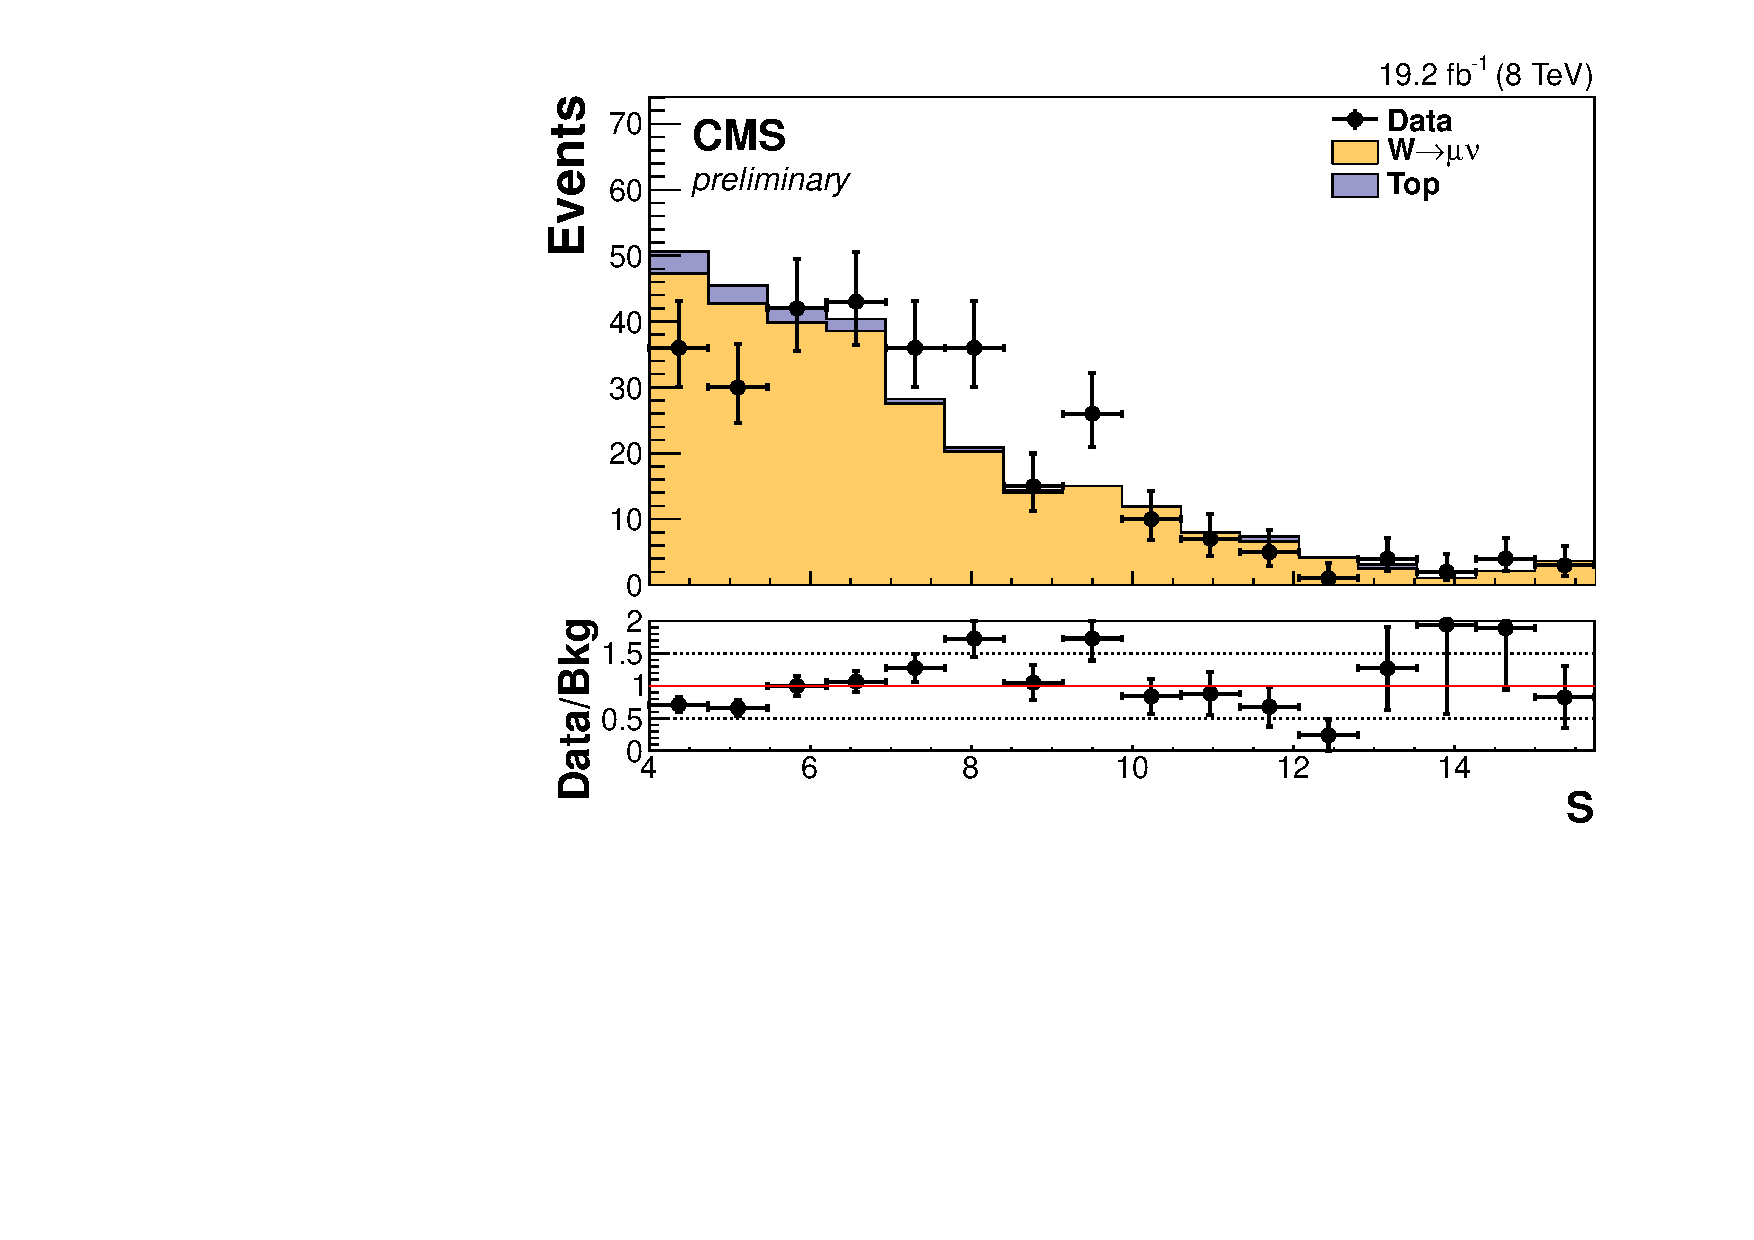
\includegraphics[width=.65\largefigwidth]{plots/parked/HIG-14-038-figs/output_sigreg/munu_metnomu_significance.pdf}

  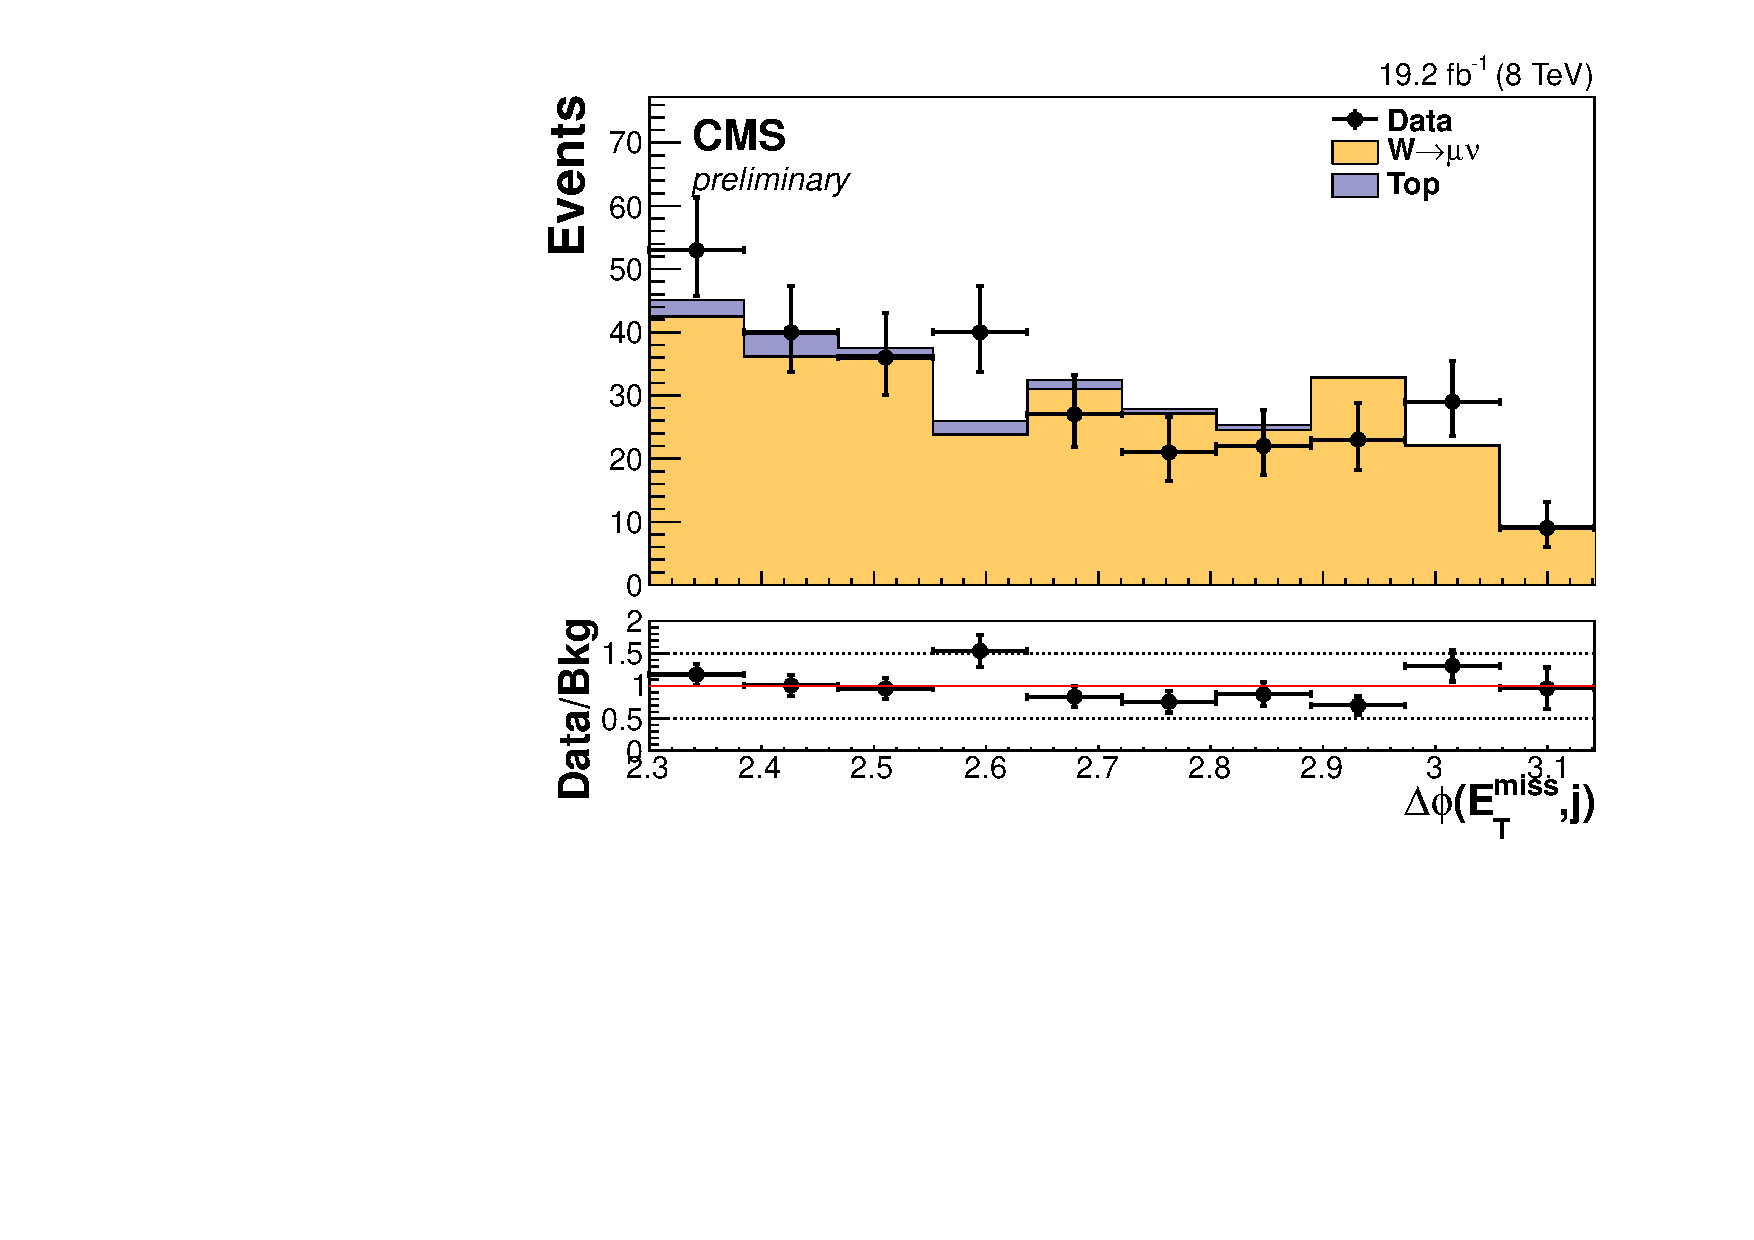
\includegraphics[width=.65\largefigwidth]{plots/parked/HIG-14-038-figs/output_sigreg/munu_alljetsmetnomu_mindphi.pdf}
    \caption{Distributions of variables in data and \ac{MC} events in the $\PW\rightarrow \mu\nu$ control region. \ac{MC} events from V+jets backgrounds are scaled by their data-driven scale factors. The variables shown are from top to bottom and left to right \detajj, \Mjj, the leading and sub-leading jet's \pt, \METnoMU, \METsig and \jetmetdphi. The last bin of each distribution contains the events above the range displayed~\cite{CMS-PAS-HIG-14-038}.}
  \label{fig:parkedwmunu}
\end{figure}

\begin{table}[h!]
  \begin{center}
    \caption{The inputs to, and results of, \EquationRef{eq:wdatabkgrep}, when used to estimate the $W\rightarrow \mu\nu$ estimate in the signal
      region.}
    \label{tab:parkedwmunu}
    \begin{tabular}{lcc}
      \hline
      \hline
      & Signal region & Control region \\
      \hline
      \hline
      $N_{Data}$&N/A&$300\pm 17.3$\stat\\
      $N_{Bkg}$&N/A&$14.8\pm 2.5(\rm{MC\,stat})$\\
      $N_{MC}$&$143.7\pm10.2(\rm{MC\,stat})$&$399.9\pm 14.9(\rm{MC\,stat})$\\
      \hline
      $\frac{N^{data}-N^{bkg}}{N^{MC}_{C}}$ & \multicolumn{2}{c|}{$0.71\pm0.04$\stat$\pm0.03$(MC stat)} \\
      \hline
      $N_{\PW\rightarrow\mu\nu}$&\textcolor{red}{$102.5\pm6.2$\stat$\pm11.7$\syst}&N/A \\
      \hline
      \hline
    \end{tabular}
  \end{center}
\end{table}



\subsection{W$\rightarrow \tau\nu$+jets}
\label{sec:parkedwtaunu}
The signal region requirements do not include a veto of hadronic taus, due to the low identification efficiency and relatively high probability for a jet to be identified as a fake tau. Requiring that there is an identified hadronic tau in addition to the signal region selection results in a region containing only 2 data events. In order to increase the number of events in the tau control region the \jetmetdphi cut was removed. The requirement that there is an identified tau reduces the \ac{QCD} multijet contribution in the low \jetmetdphi region significantly compared to what was seen during the choice of the preselection. However, poor data-\ac{MC} agreement was still observed in the \jetmetdphi$<1$ region, which is evidence that some events from multijet processes are still present. To remove these \ac{QCD} multijet events, whilst keeping a reasonable number of events in the resulting control region, a requirement that \jetmetdphileading is greater than 1 and that the transverse mass of the hadronic tau and \MET system is greater than 20 \GeV is applied. The \jetmetdphileading requirement reduces \ac{QCD} backgrounds for the same reason that \jetmetdphi does, but it is a slightly looser requirement as it only considers the two leading jets. The transverse mass of the tau-\MET system is a good variable to reject \ac{QCD} where a lepton is present as in real \PW boson events the tau and \MET are expected to originate from the same object and therefore have significant invariant mass, which is not the case for \ac{QCD} multijet events.

After the anti-\ac{QCD} cuts the agreement between data and \ac{MC} is good as can be seen in \FigureRef{fig:parkedwtaunu}. To account for the different \jetmetdphi selection in this region and the signal region, the data driven scale factor was calculated both in the $\PW\rightarrow\mu\nu$ control region, which has the signal region \jetmetdphi selection, and in a modified single muon control region with the $\PW\rightarrow\tau\nu$ control region \jetmetdphi selection. The difference between these two scale factors was found to be 20\%, so a 20\% systematic uncertainty was added to the estimate of the $\PW\rightarrow\tau\nu$ background.

The single tau control region with a \jetmetdphileading cut and no \jetmetdphi cut was used with \EquationRef{eq:wdatabkgrep} to estimate the number of $\PW\rightarrow\tau\nu$ events in the signal region. A table of the inputs to, and results of, \EquationRef{eq:wdatabkgrep} can be seen in \TableRef{tab:parkedwtaunu}. The contribution from other backgrounds in the $\PW\rightarrow\tau\nu$ control region is approximately 15\%, with most of these other background events being due to top quark related processes. The scale factor obtained for this background is 0.78, which is closer to 1 than those seen in the other $\PW+$jets backgrounds, however it also has the largest uncertainty. Further investigation of the V+jets scale factors is detailed in \SectionRef{sec:parkedscalefactors}.

\begin{figure}
  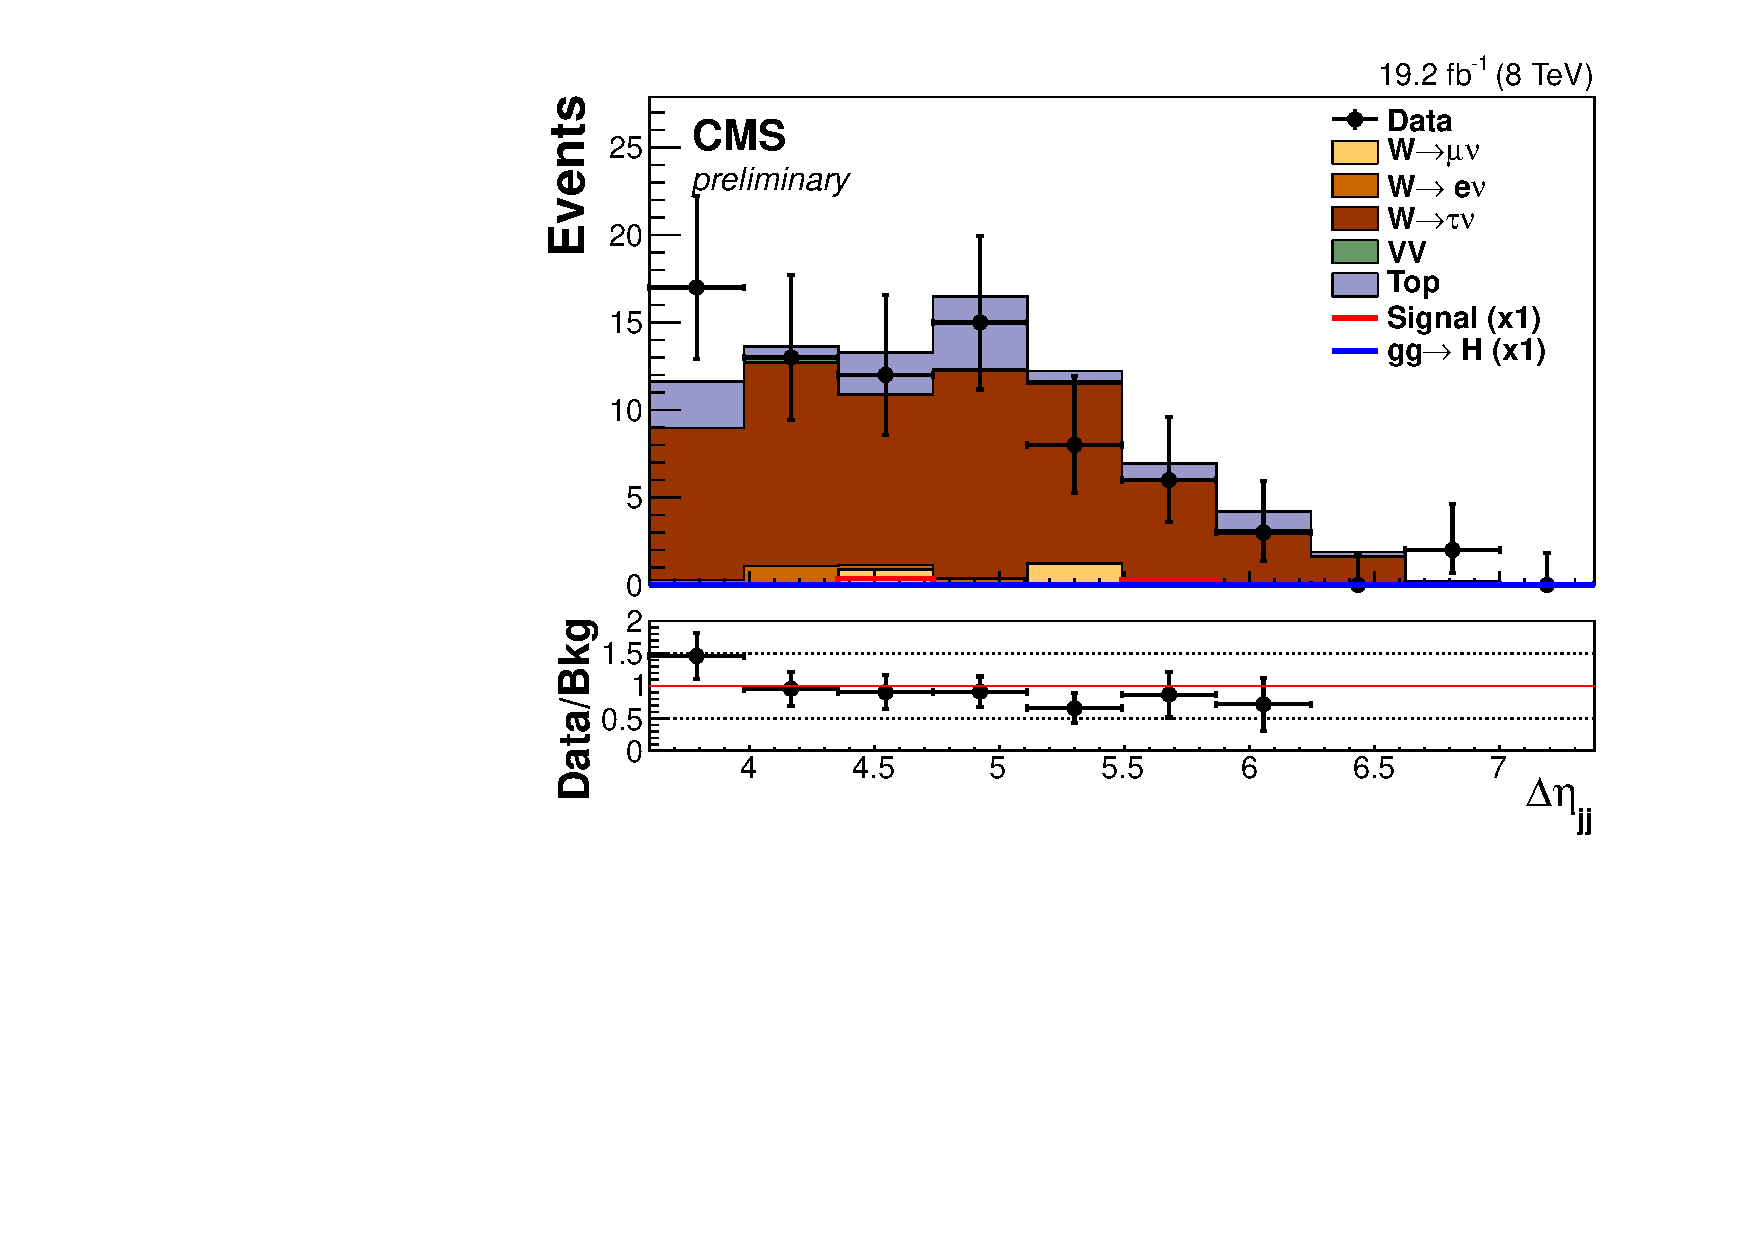
\includegraphics[width=.65\largefigwidth]{plots/parked/HIG-14-038-figs/output_sigreg/taunu_dijet_deta.pdf}
  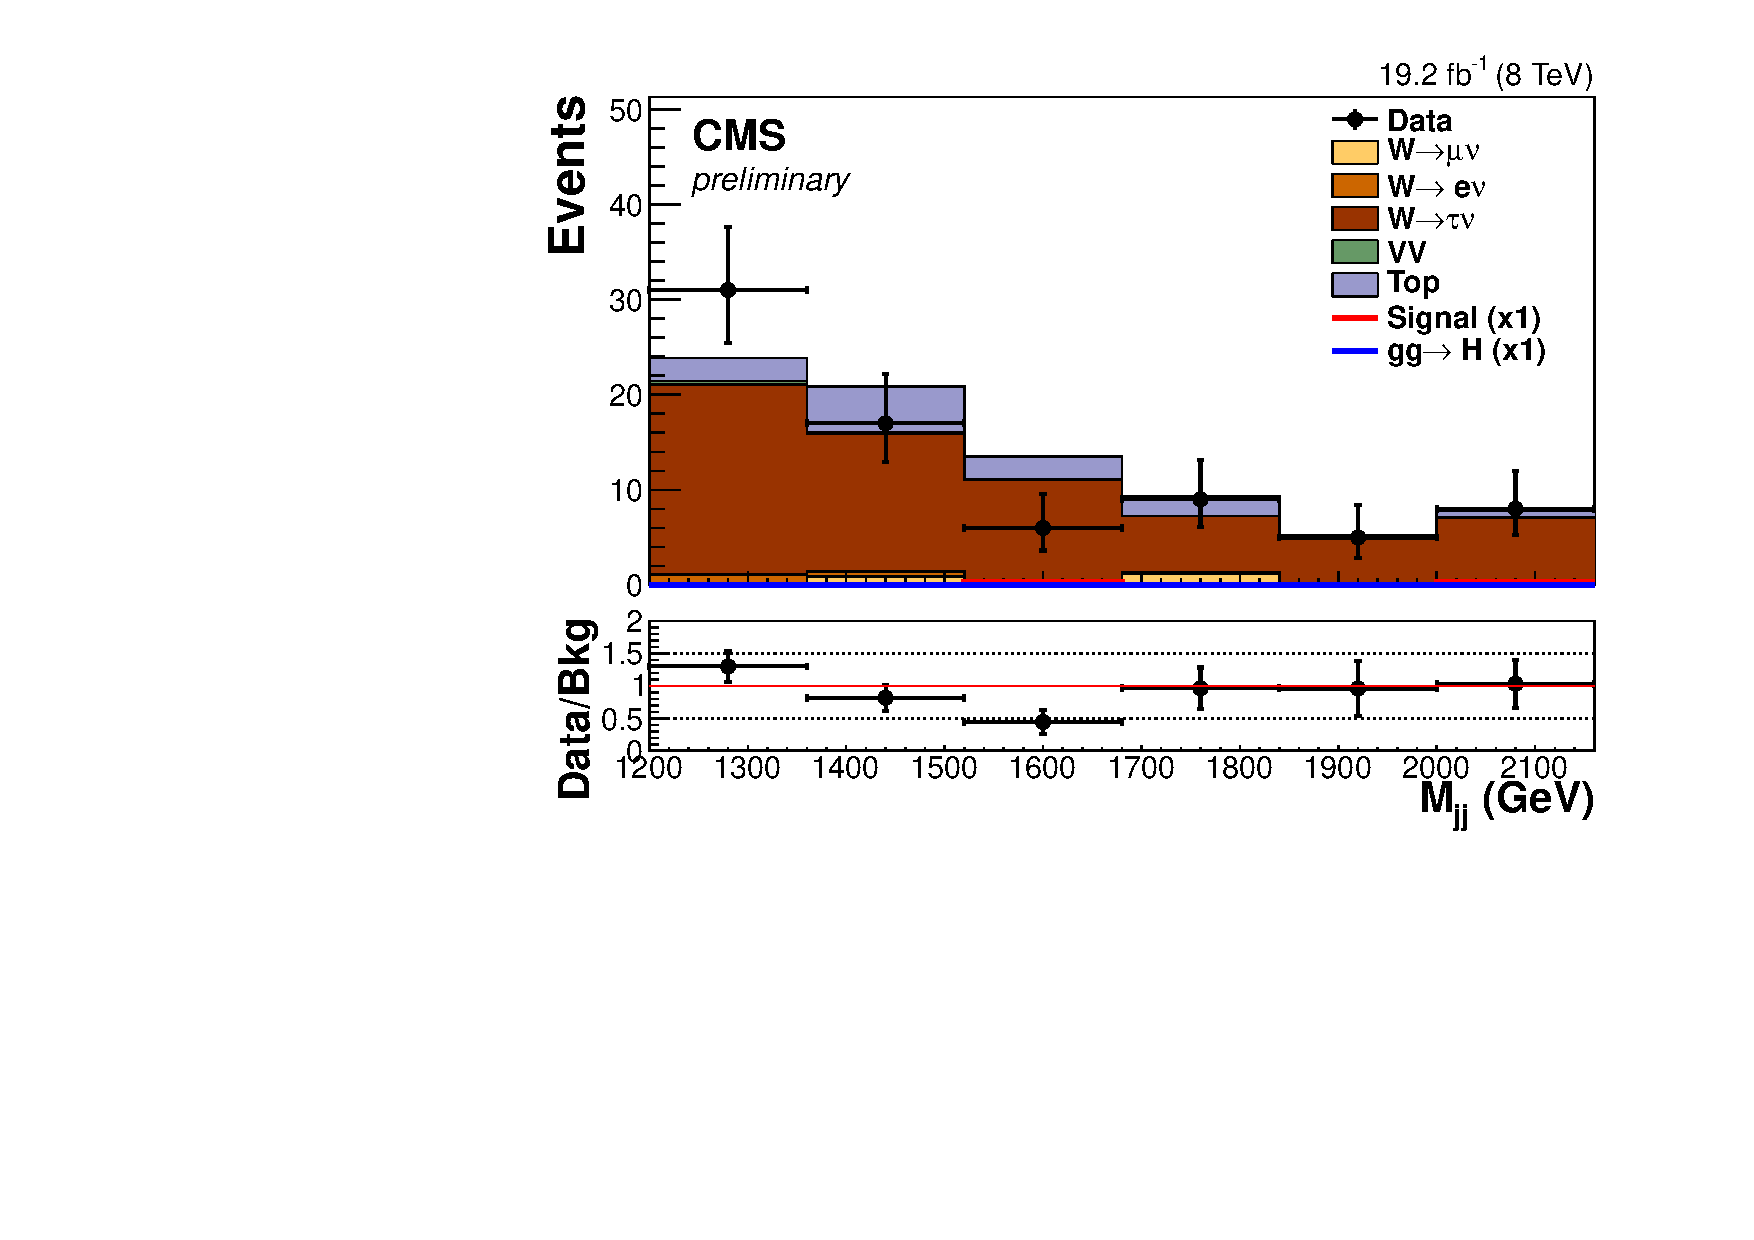
\includegraphics[width=.65\largefigwidth]{plots/parked/HIG-14-038-figs/output_sigreg/taunu_dijet_M.pdf}

  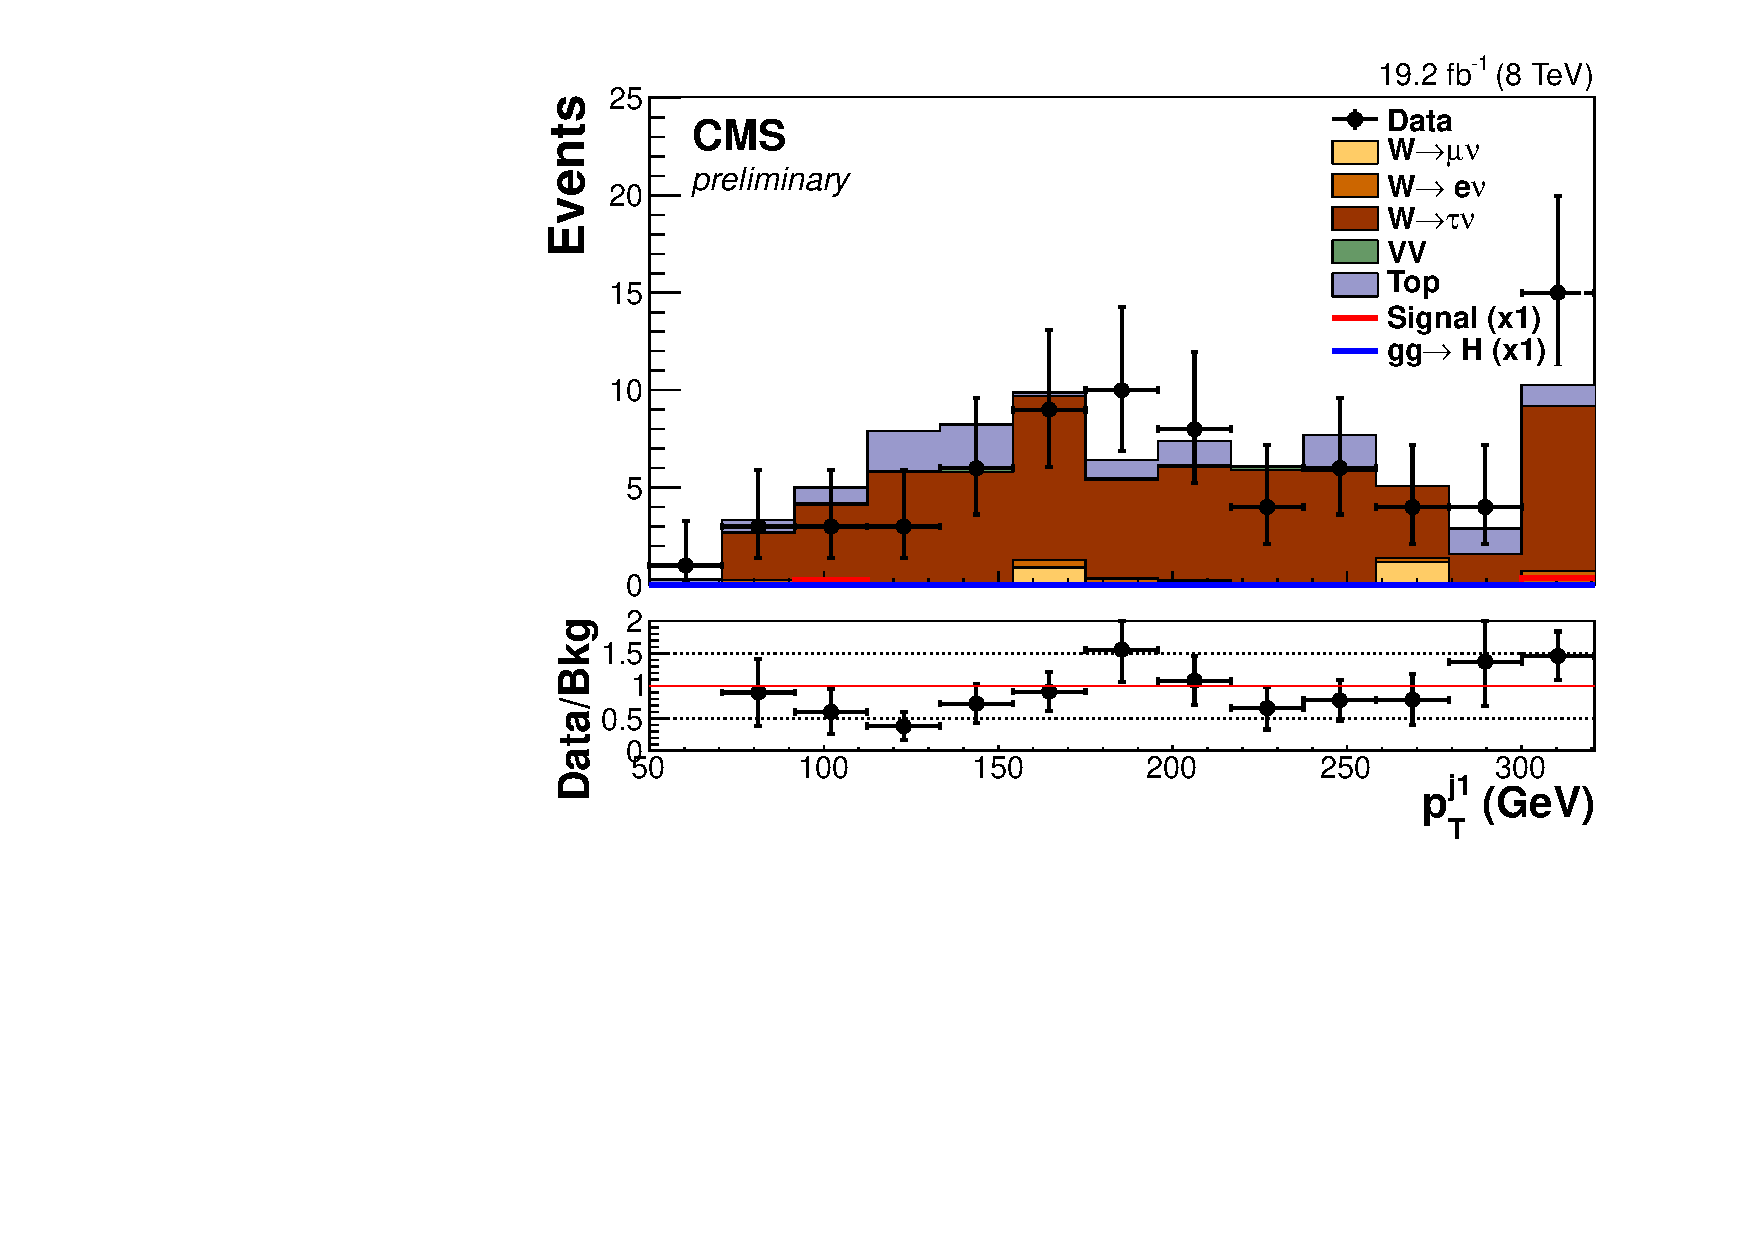
\includegraphics[width=.65\largefigwidth]{plots/parked/HIG-14-038-figs/output_sigreg/taunu_jet1_pt.pdf}
  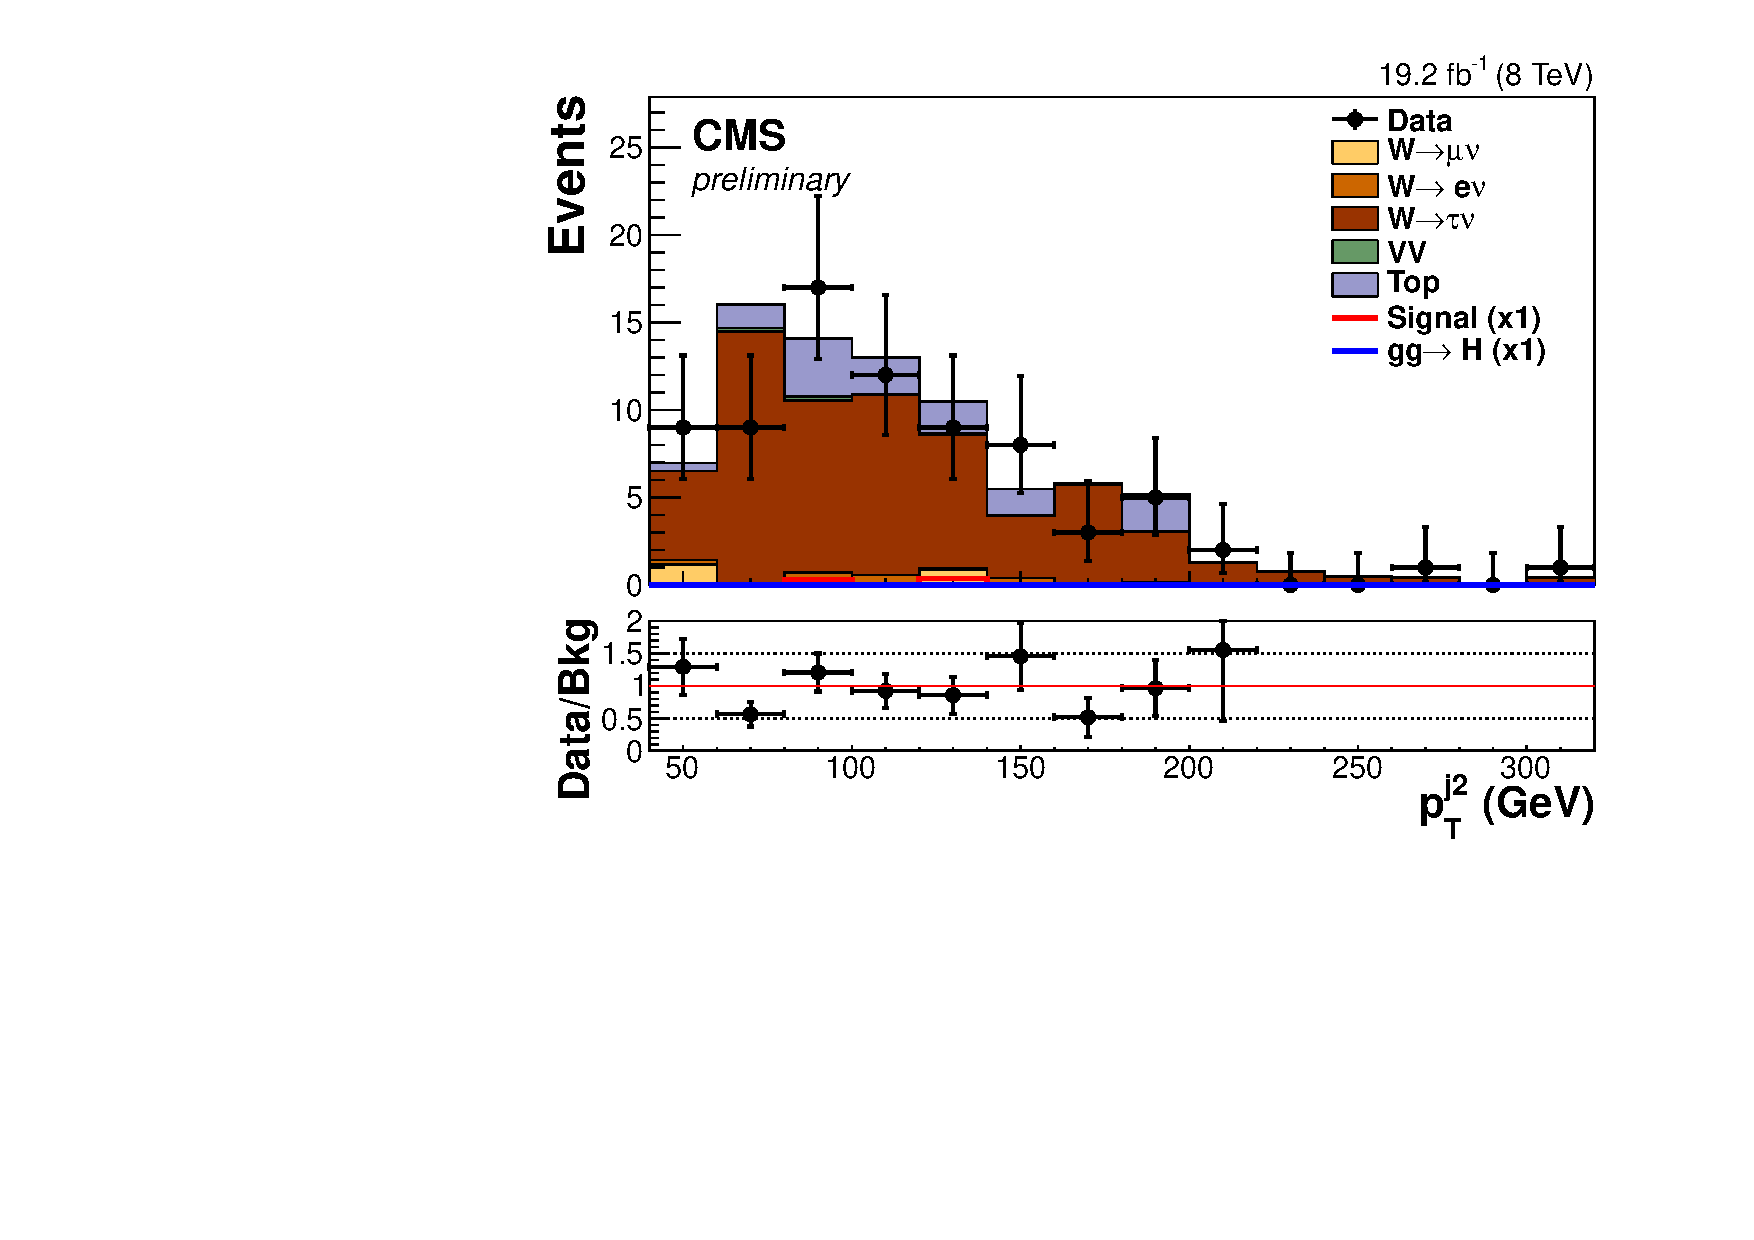
\includegraphics[width=.65\largefigwidth]{plots/parked/HIG-14-038-figs/output_sigreg/taunu_jet2_pt.pdf}

  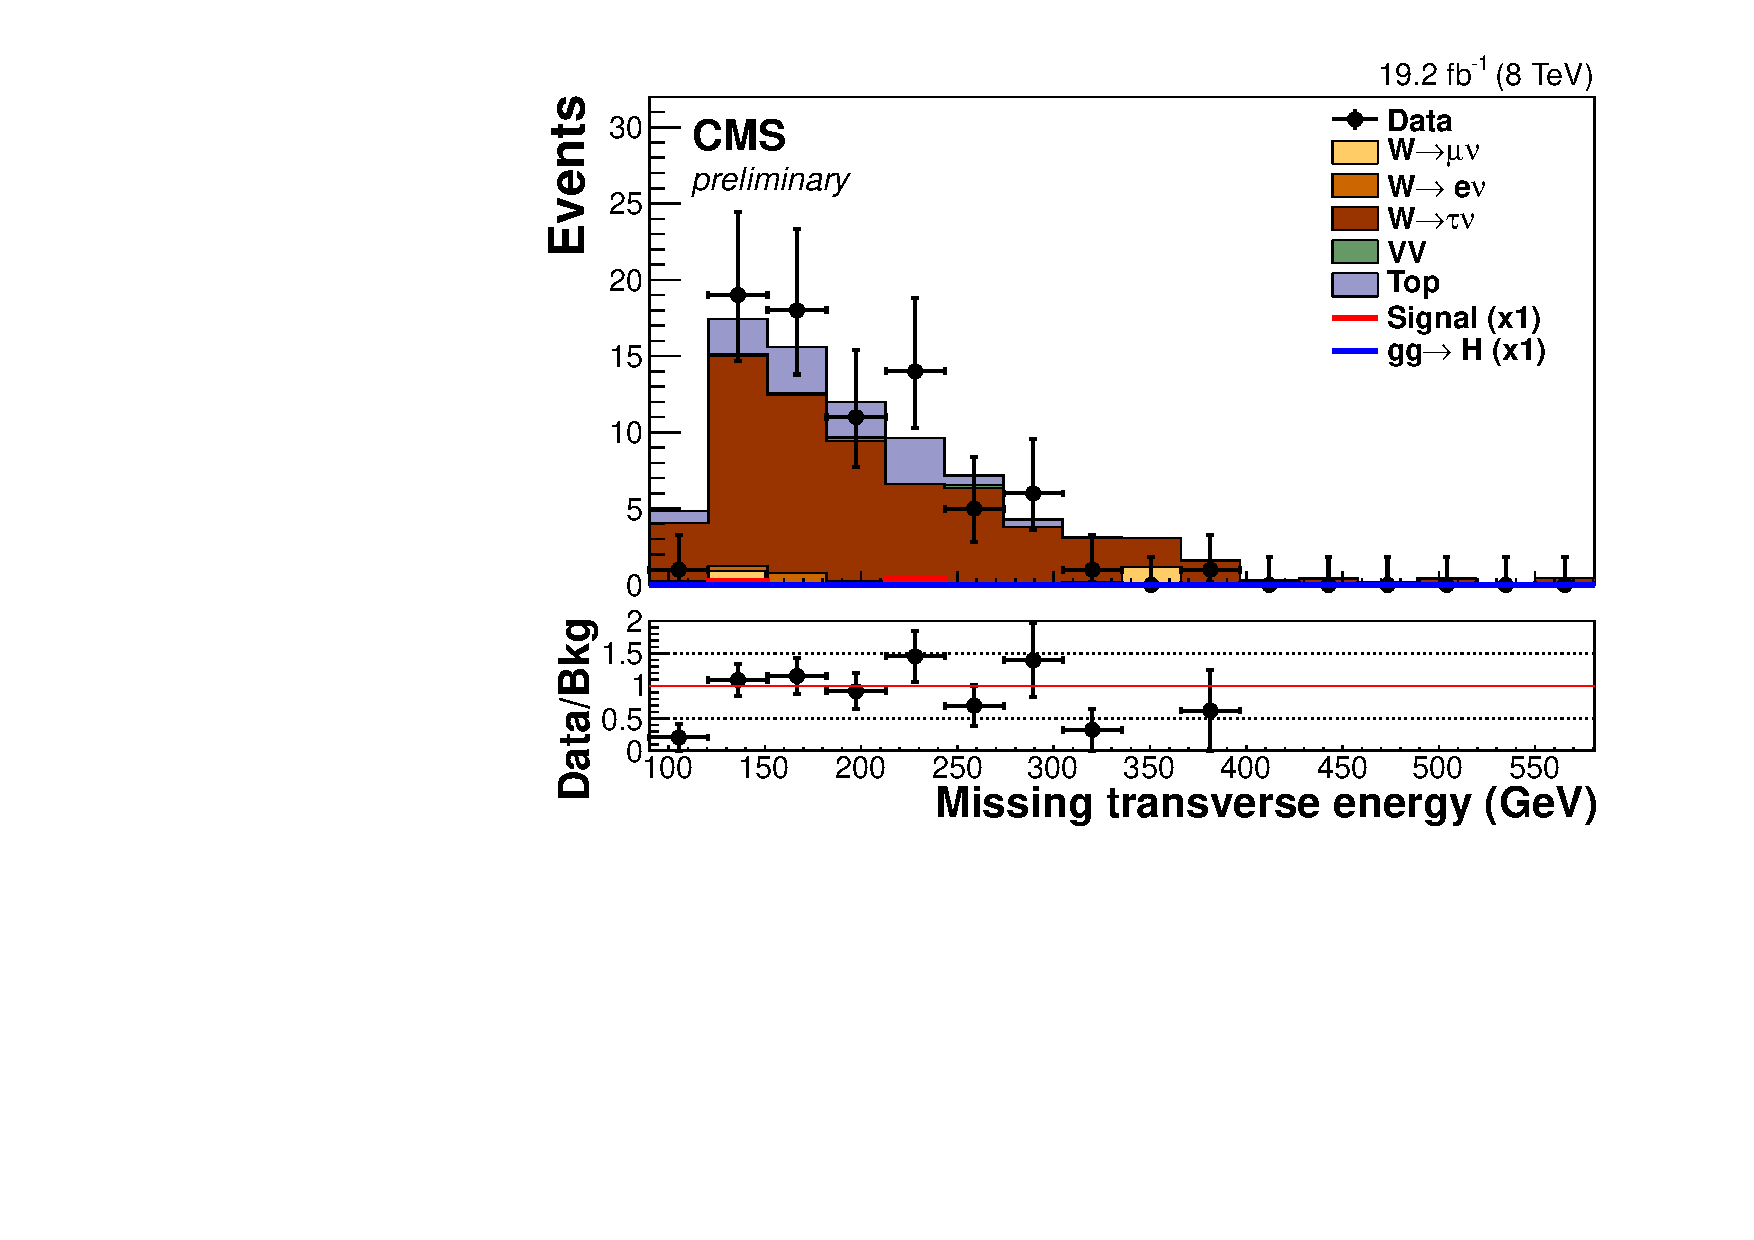
\includegraphics[width=.65\largefigwidth]{plots/parked/HIG-14-038-figs/output_sigreg/taunu_metnomuons.pdf}
  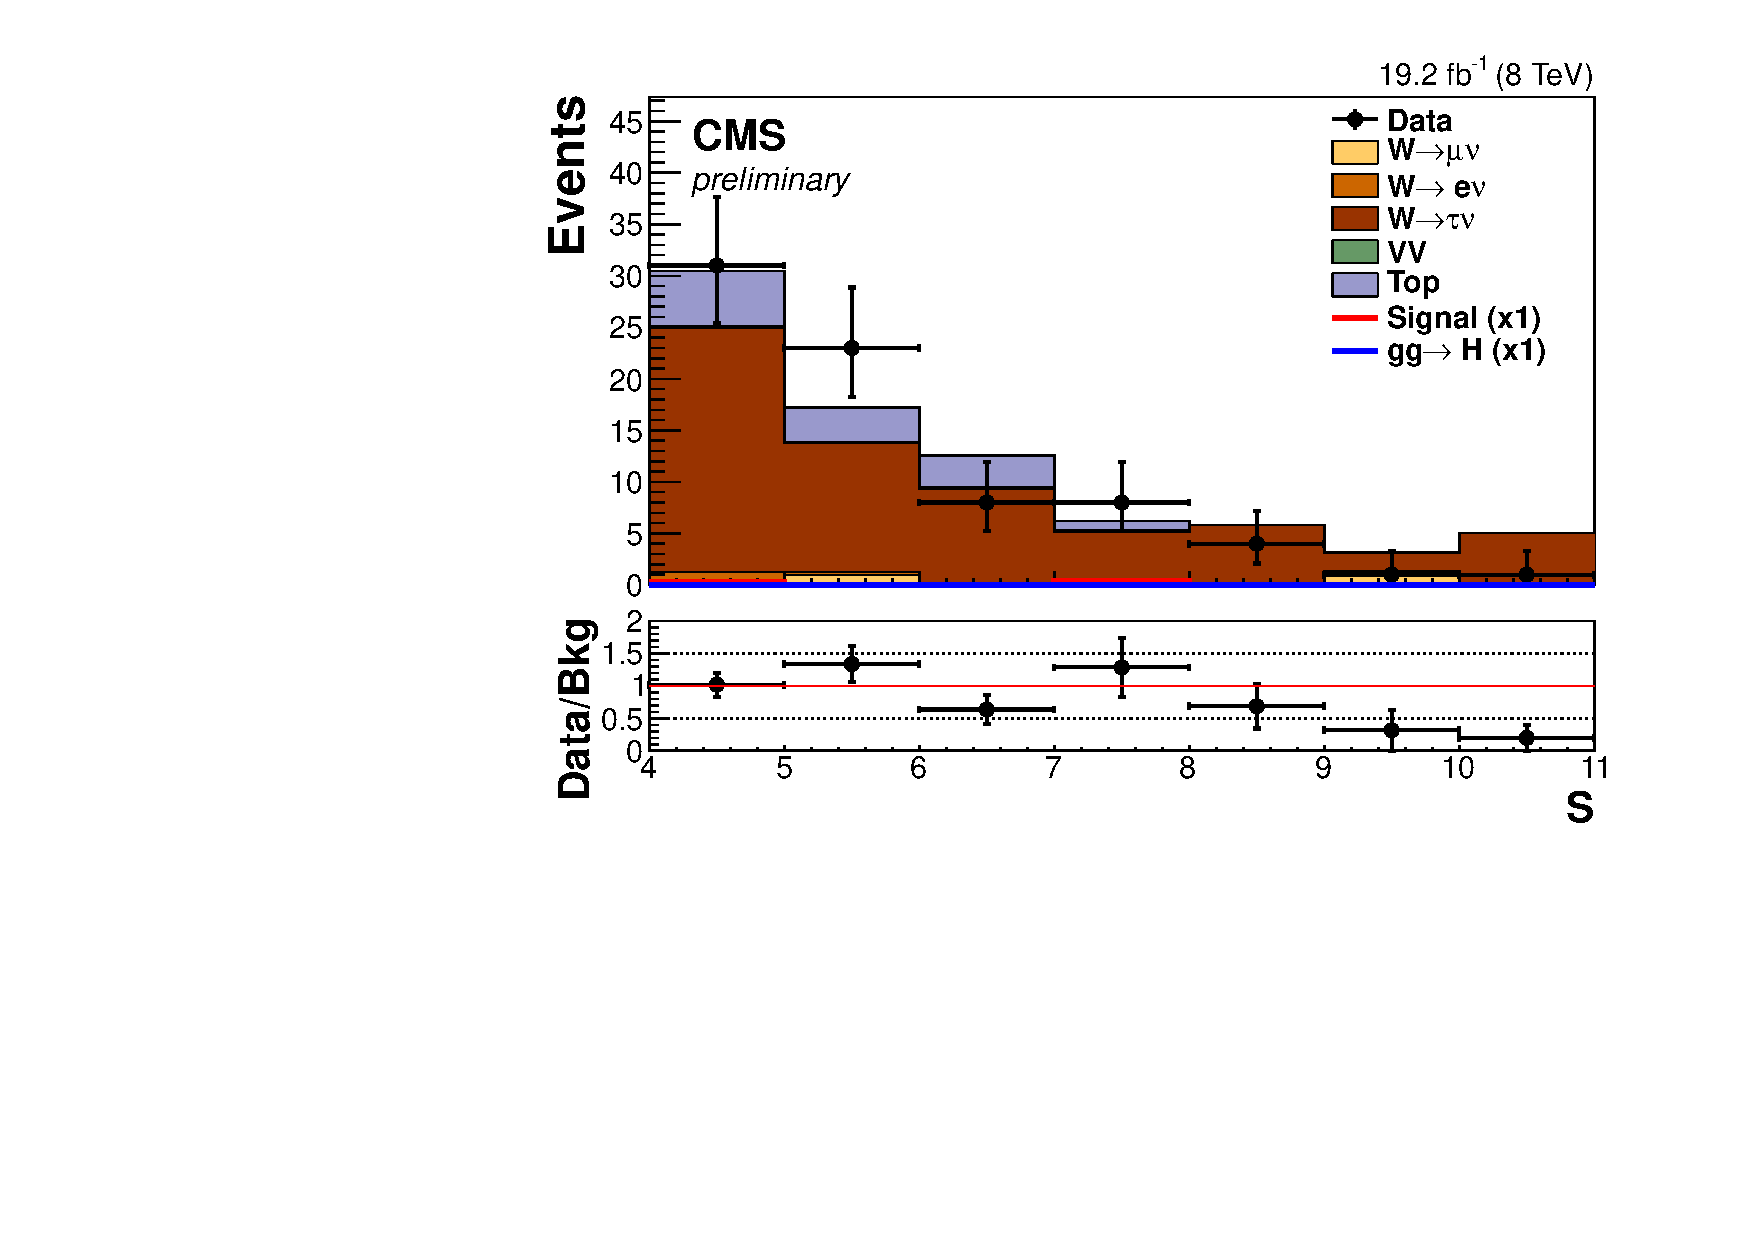
\includegraphics[width=.65\largefigwidth]{plots/parked/HIG-14-038-figs/output_sigreg/taunu_metnomu_significance.pdf}

  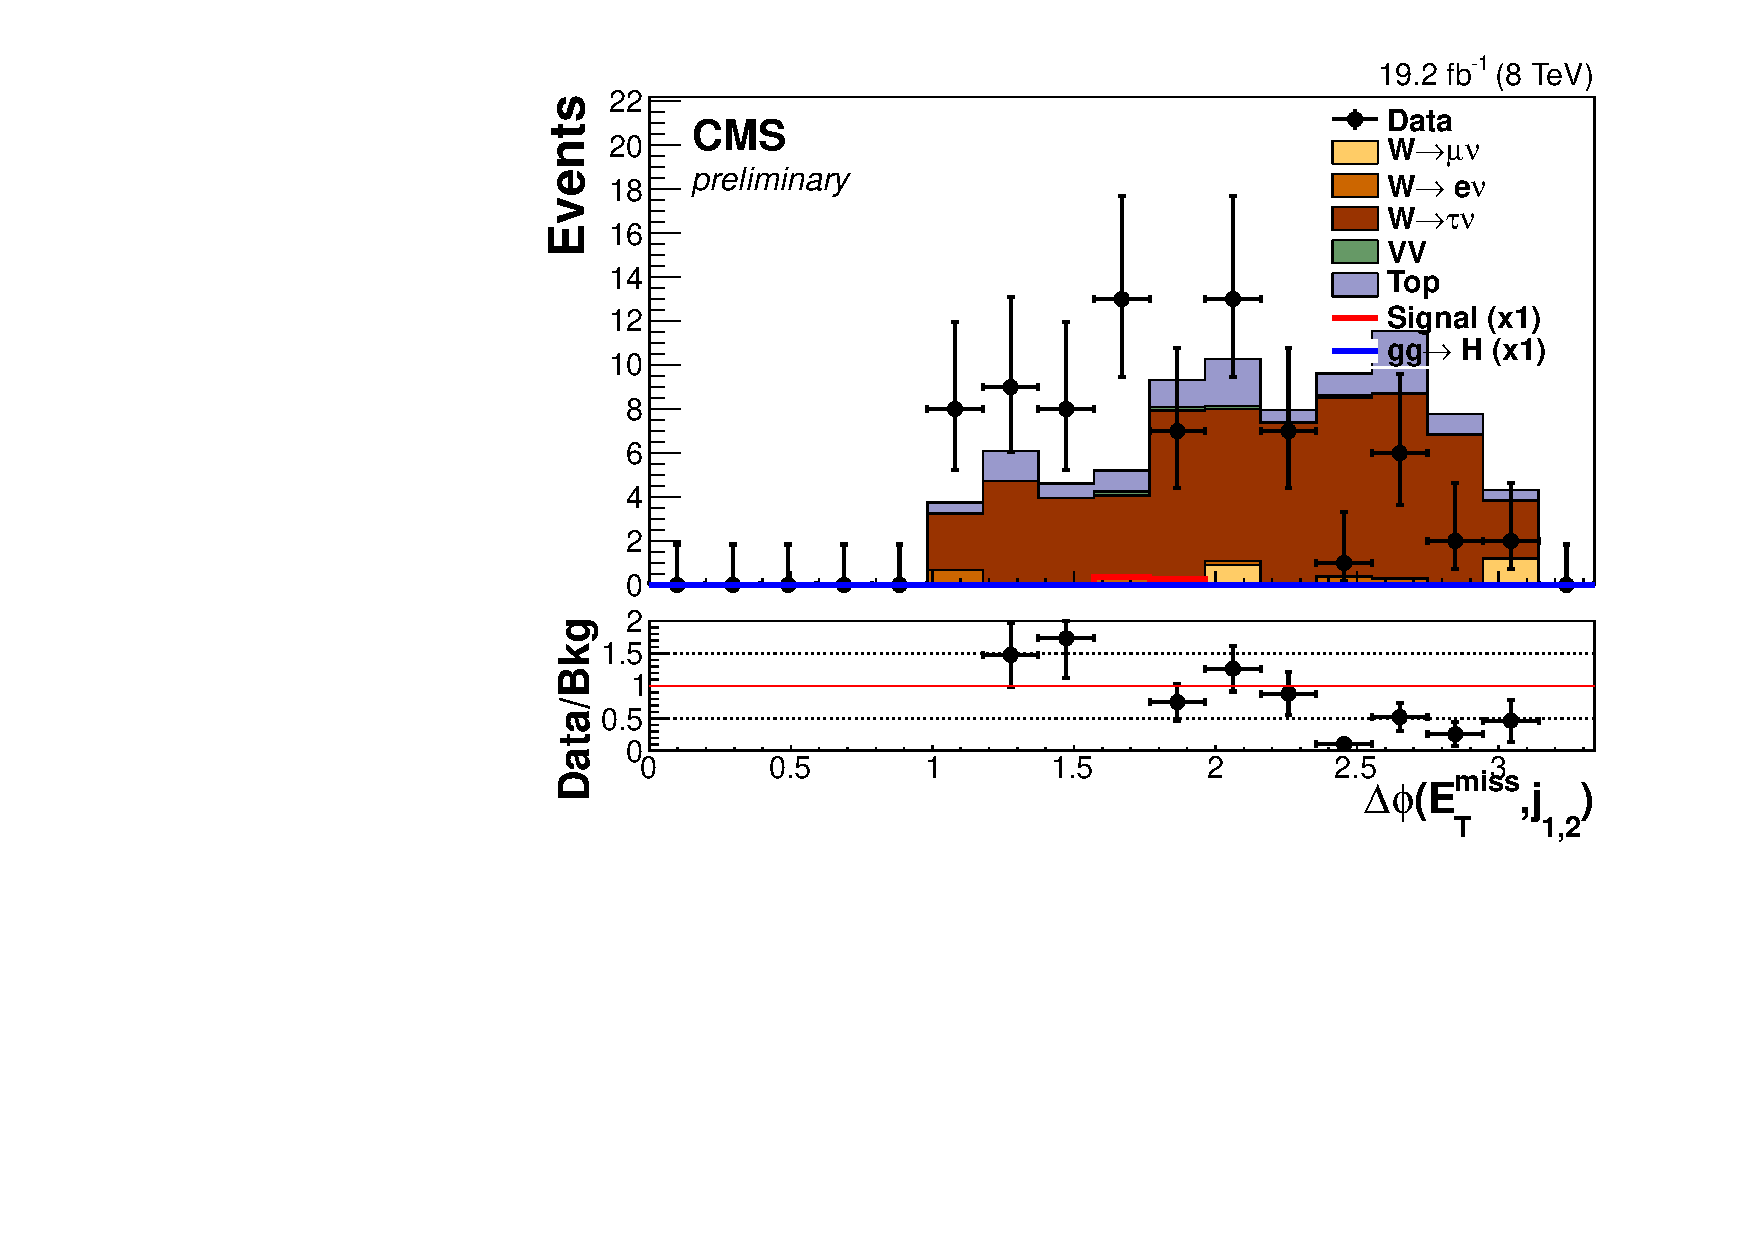
\includegraphics[width=.65\largefigwidth]{plots/parked/HIG-14-038-figs/output_sigreg/taunu_jetmetnomu_mindphi.pdf}
  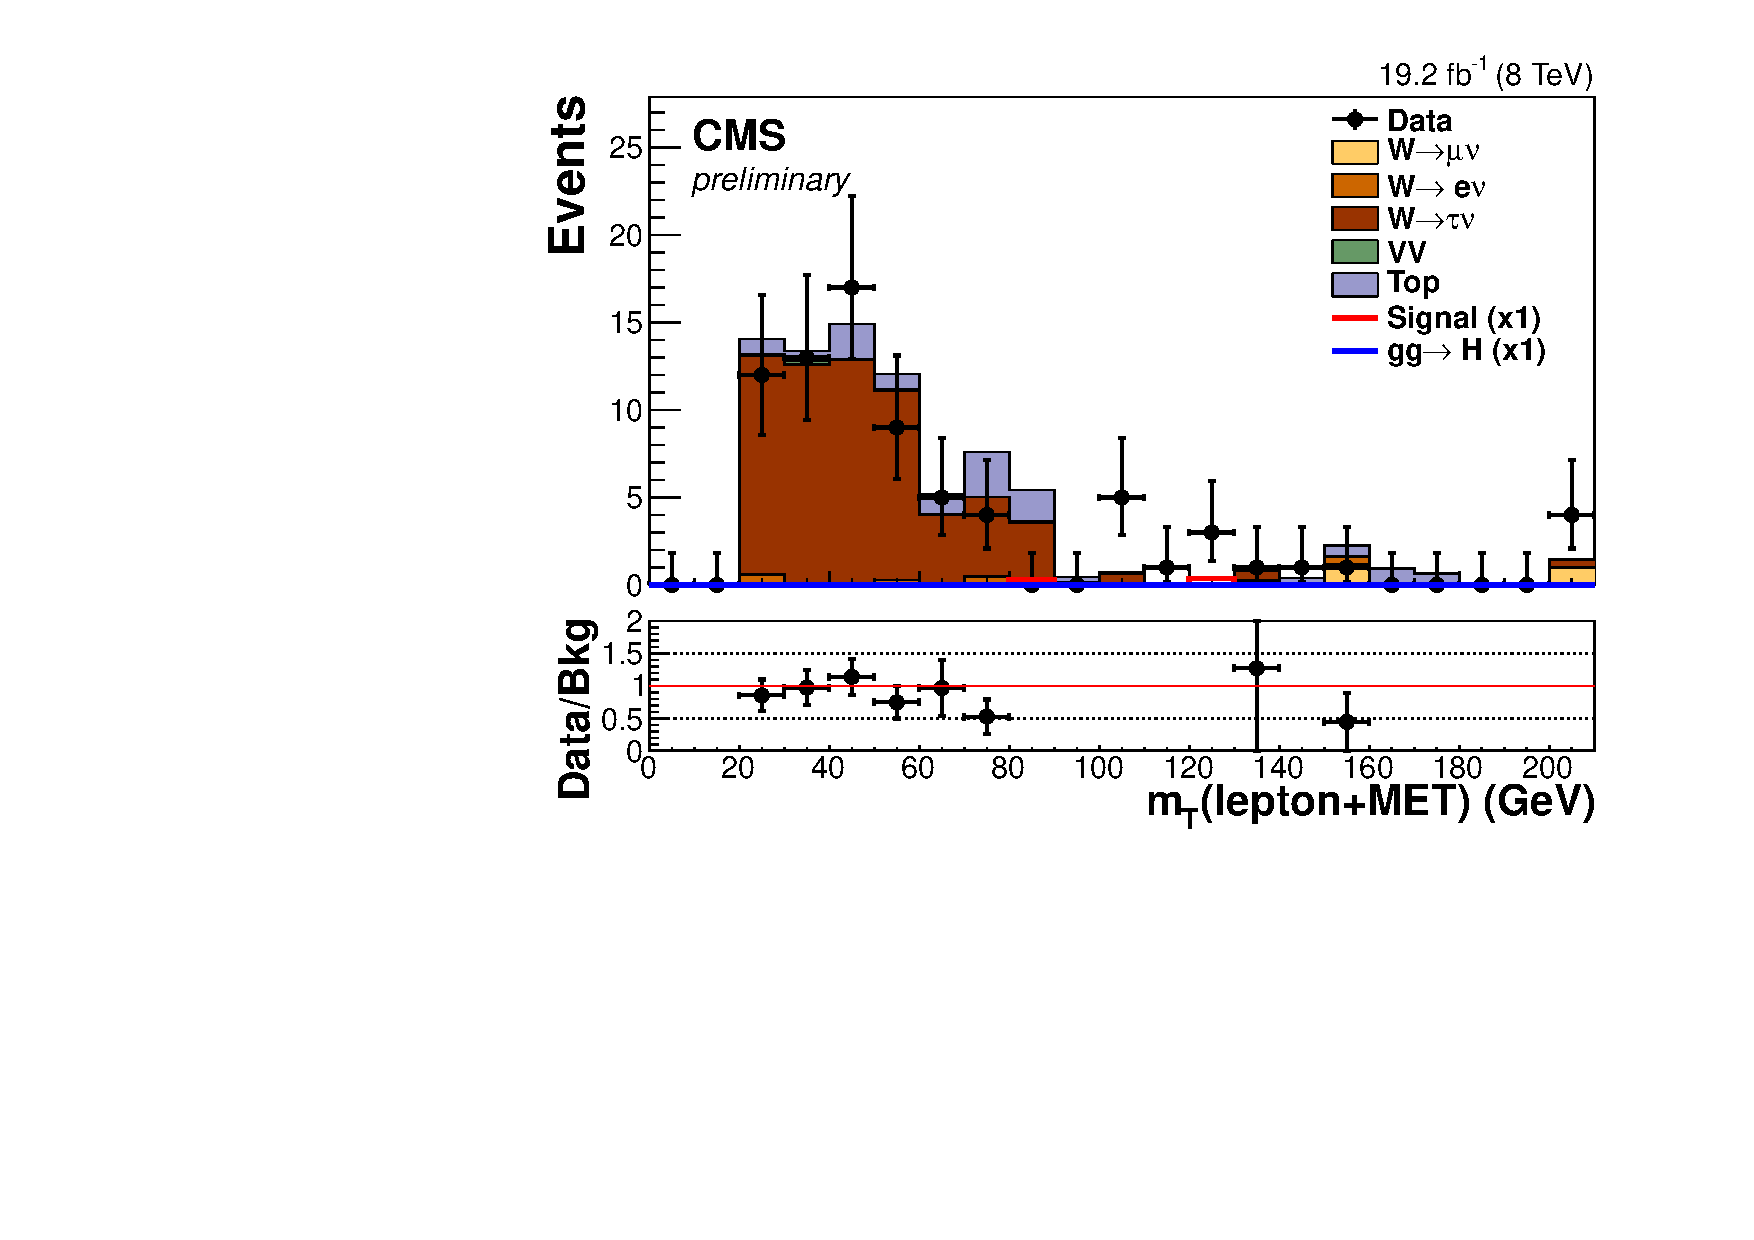
\includegraphics[width=.65\largefigwidth]{plots/parked/HIG-14-038-figs/output_sigreg/taunu_lep_mt.pdf}
  \caption{Distributions of variables in data and \ac{MC} events in the $\PW\rightarrow \tau\nu$ control region. \ac{MC} events from V+jets backgrounds are scaled by their data-driven scale factors. The variables shown are from top to bottom and left to right \detajj, \Mjj, the leading and sub-leading jet's \pt, \METnoMU, \METsig, \jetmetdphileading and the tau-\MET system's transverse mass. The last bin of each distribution contains the events above the range displayed~\cite{CMS-PAS-HIG-14-038}.}
  \label{fig:parkedwtaunu}
\end{figure}

\begin{table}[h!]
  \begin{center}
    \caption{The inputs to, and results of, \EquationRef{eq:wdatabkgrep}, when used to estimate the $W\rightarrow \tau\nu$ estimate in the signal
      region.}
    \label{tab:parkedwtaunu}
    \begin{tabular}{lcc}
      \hline
      \hline
      & Signal region & Control region \\
      \hline
      \hline
      $N_{Data}$&N/A&$76\pm 8.7$\stat\\
      $N_{Bkg}$&N/A&$13.3\pm 2.8(\rm{MC\,stat})$\\
      $N_{MC}$&$121.9\pm 8.7(\rm{MC\,stat})$&$80.8\pm 6.4(\rm{MC\,stat})$\\
      \hline
      $\frac{N^{data}-N^{bkg}}{N^{MC}_{C}}$ & \multicolumn{2}{c|}{$0.78\pm 0.11$\stat$\pm 0.07$(MC stat)} \\
      \hline
      $N_{\PW\rightarrow\mu\nu}$&\textcolor{red}{$94.6\pm 13.1$\stat$\pm 23.8$\syst}&N/A \\
      \hline
      \hline
    \end{tabular}
  \end{center}
\end{table}



\subsection{Differences between the $W\rightarrow e\nu$, $W\rightarrow\mu\nu$ and $W\rightarrow\tau\nu$ +jets backgrounds}
\label{sec:parkedenumunudiff}
%tau easily explainable by id eff
%sf for enu and munu different but compatible MC yield is where main difference is separate into into and out of acceptance and why (electrons in HF are jets, electron ID eff slightly worse) mindphijetmet shape difference outside acceptance
The number of W+jets events decaying to a particular flavour of lepton with \ac{VBF}-like jet kinematics should be the same for all three flavours of lepton through lepton universality. Differences between the numbers of background events from $\PW\rightarrow e\nu$, $\PW\rightarrow \mu\nu$ and $\PW\rightarrow \tau\nu$ must therefore be due to differences in the identification of the leptons. Hadronic taus have much lower identification efficiencies than the other two flavours of leptons, so might naively be expected to give rise to a much larger number of background events. However, due to the similarities between hadronic taus and jets, unidentified taus often lead to additional jets in the event and therefore increase the probability that an event will fail the \jetmetdphi cut~\cite{CMS-PAS-TAU-11-001}. These two competing effects mean that the number of background events from $\PW\rightarrow\tau\nu$ passing the signal region selection is not necessarily expected to be the same as that from $\PW\rightarrow e\nu$ and $\PW\rightarrow\mu\nu$.

By contrast, electrons and muons have much more similar identification efficiencies (see Sections~\ref{sec:electrons} and \ref{sec:muons}). The 45\% difference seen in the number of expected background events from these two processes was therefore unexpected. This difference was also not seen in the prompt analysis, as can be seen from \TableRef{tab:promptresults}. The prediction of the $\PW\rightarrow e/\mu\nu$ backgrounds is made up of a data driven scale factor and an estimate from \ac{MC} of the number of events from the process expected in the signal region, $N_{MC}^{S}$. Both these elements were studied to try to understand the observed differences.

Firstly, the data driven scale factors for the electron and muon backgrounds differ by 30\%, which is not sufficient to explain the full difference between the electron and muon background estimates. Furthermore, when systematic errors are taken into account this difference is only approximately one standard deviation. On the other hand, $N_{MC}^{S}$ does show a significant difference.

To study the difference in $N_{MC}^{S}$ two sub-regions of the signal region were studied, that with a generator level lepton inside the detector acceptance for both electrons and muons ($|\eta<2.1$), and that with a generator lepton outside the detector acceptance for both electrons and muons ($|\eta|>2.4$). The number of events in these two sub-regions from both $\PW\rightarrow e\nu$ and $\PW\rightarrow\mu\nu$ \ac{MC} can be seen in \TableRef{tab:enumunudiff}. The numbers of events with a generator level lepton inside acceptance are approximately one standard deviation higher for electrons. This small difference is expected due to the lower identification efficiency for veto leptons making them less likely to cause an event to fail the lepton veto. Distributions of several variables were also studied for events inside the acceptance and found to be very similar for both $\PW\rightarrow e\nu$ and $\PW\rightarrow\mu\nu$ events.

Outside the acceptance there are a lot more muon events than electron events. In this region neither flavour of lepton can be reconstructed and therefore cannot lead to an event failing the lepton veto, which implies that any difference is due to one or both flavours of lepton being reconstructed as a different object and affecting the jet or \MET related variables in the signal region selection. To study this effect further, the \jetmetdphi requirement was relaxed to 1 and the distributions of several variables plotted for electron and muon events outside the acceptance. Three of these distributions are shown in \FigureRef{fig:enumunudiff}. It can be seen from \FigureRef{fig:enumunudiff}a that electron events generally have more jets than muon events. \FigureRef{fig:enumunudiff}b indicates that the electron events also have much lower values of \jetmetdphi. Finally, \FigureRef{fig:enumunudiff}c shows that there are very few events passing this region's selection requirements which have a generator level electron with \pt$>30$ \GeV, the threshold for jets to be included in the \jetmetdphi cut. These three pieces of information suggest that electrons are being reconstructed as jets when outside acceptance significantly more often than muons are. These misreconstructed jets then cause the electron events to fail the \jetmetdphi requirement.

It is to be expected that electrons outside of the detector acceptance will be reconstructed as jets, as these electrons will only be seen as deposits in the forward \ac{HCAL} and therefore be indistinguishable from jets. By contrast, muons deposit very little energy in the calorimeter systems, so will simply not be identified if they are outside the acceptance of the muon system. In the prompt analysis, no requirements were made on jets which were further forward in $\eta$ than the tag jets, explaining why the difference in the numbers of $\PW\rightarrow e\nu$ and $\PW\rightarrow\mu\nu$ events was not seen there.

\begin{table}
  \caption{The numbers of events predicted by \ac{MC} in the two sub-regions of the signal region with a generator level lepton that is inside/outside the detector acceptance for both electrons and muons from $\PW\rightarrow e\nu$ and $\PW\rightarrow\mu\nu$ processes. The errors shown are the \ac{MC} statistical uncertainties.}
  \label{tab:enumunudiff}
  \begin{tabular}{lcc}
    \hline
    \hline
    Process & Inside acceptance & Outside acceptance \\
    \hline
    $\PW\rightarrow e\nu$ & $73.7\pm 6.8$ & $30.2\pm 4.9$ \\
    $\PW\rightarrow \mu\nu$ & $61.5\pm 6.8$ & $74.4\pm7.3$ \\
    \hline
    \hline
  \end{tabular}
\end{table}

\begin{figure}
  \subfloat[]{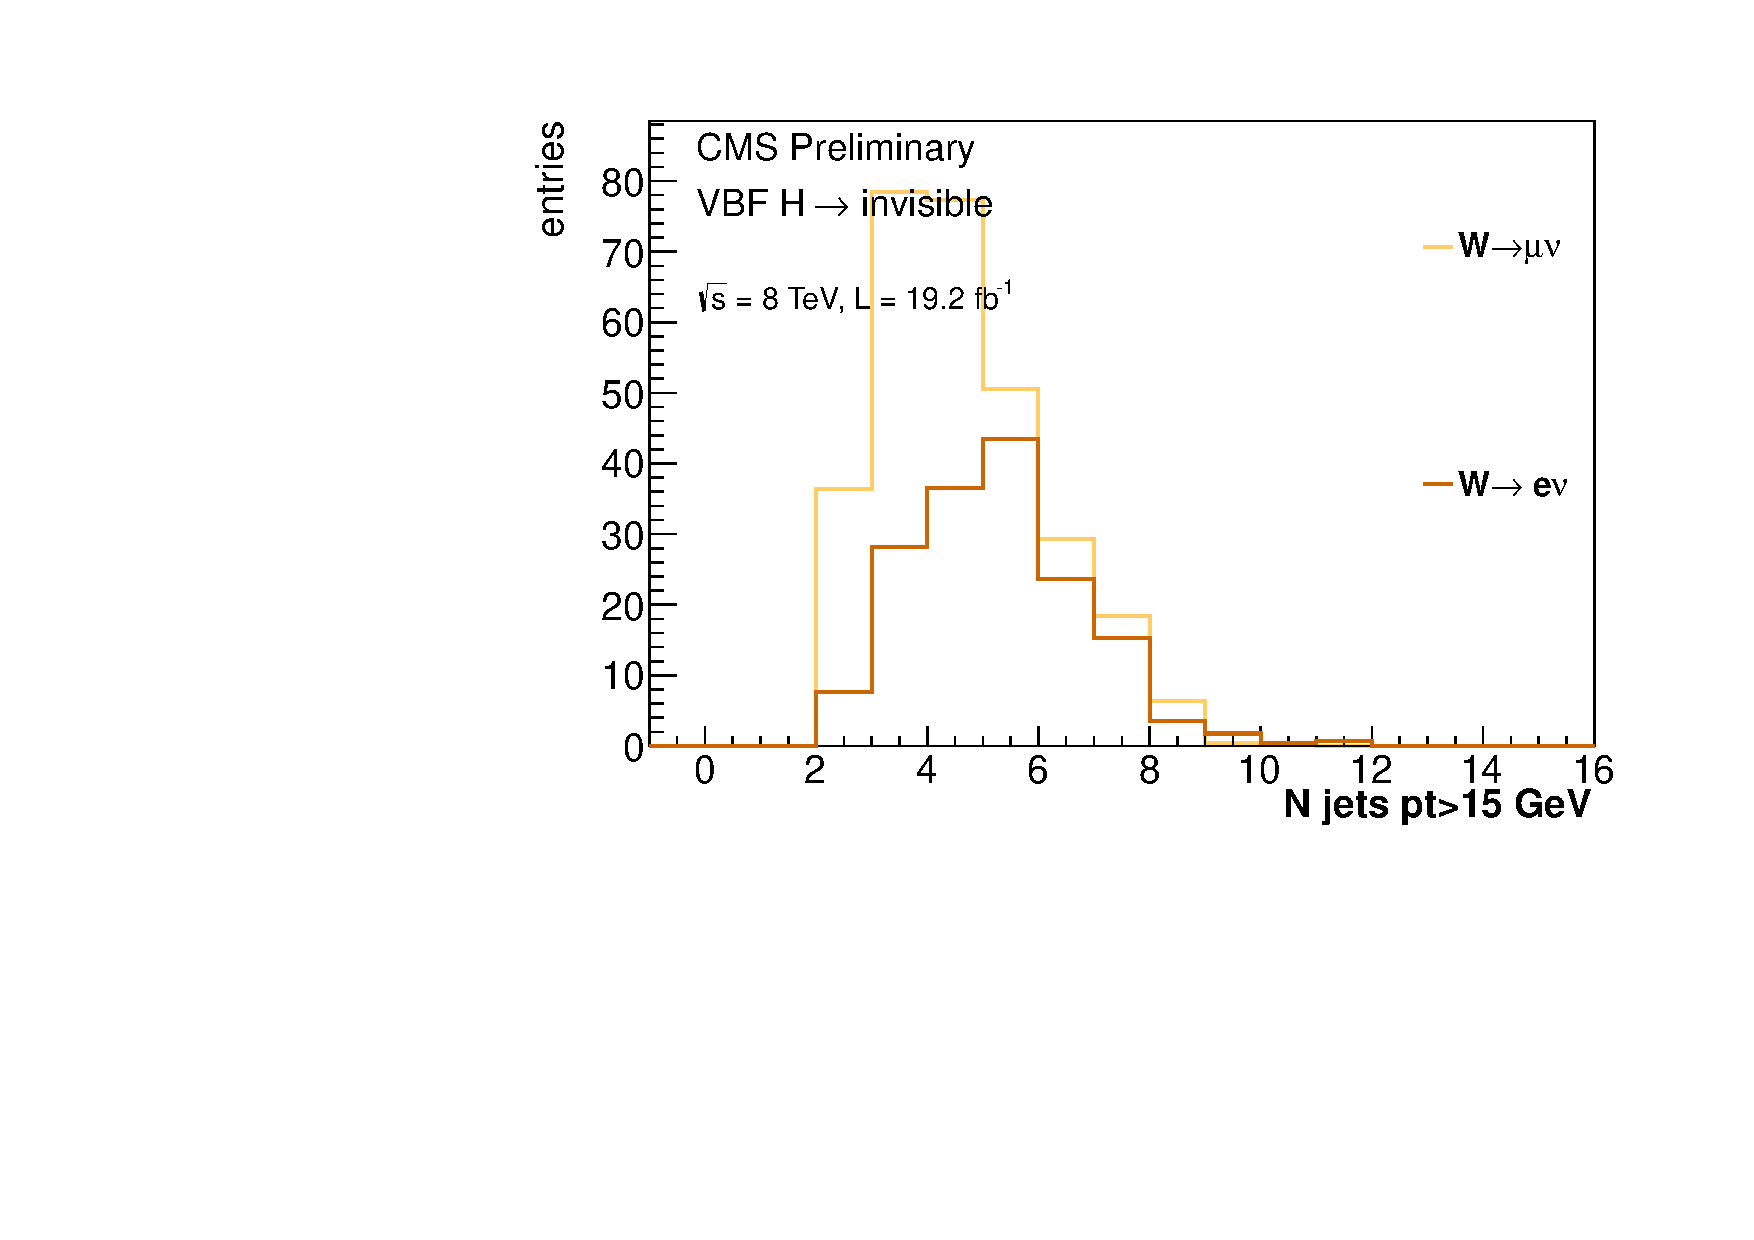
\includegraphics[width=.65\largefigwidth]{plots/parked/AN-14-243-figs/genlepstudy/outsideaccloosedphi/nunu_n_jets_15.pdf}}
  \subfloat[]{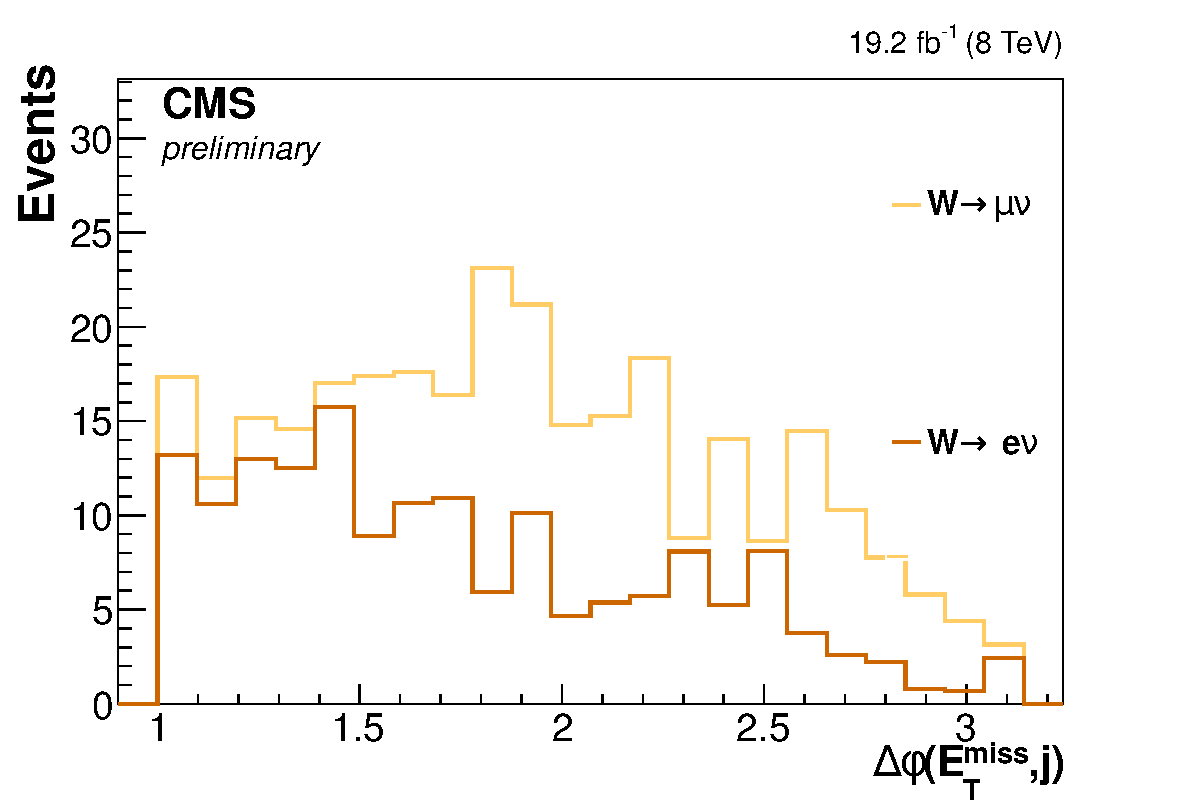
\includegraphics[width=.65\largefigwidth]{plots/parked/AN-14-243-figs/genlepstudy/outsideaccloosedphi/nunu_alljetsmetnomu_mindphi.pdf}}

  \subfloat[]{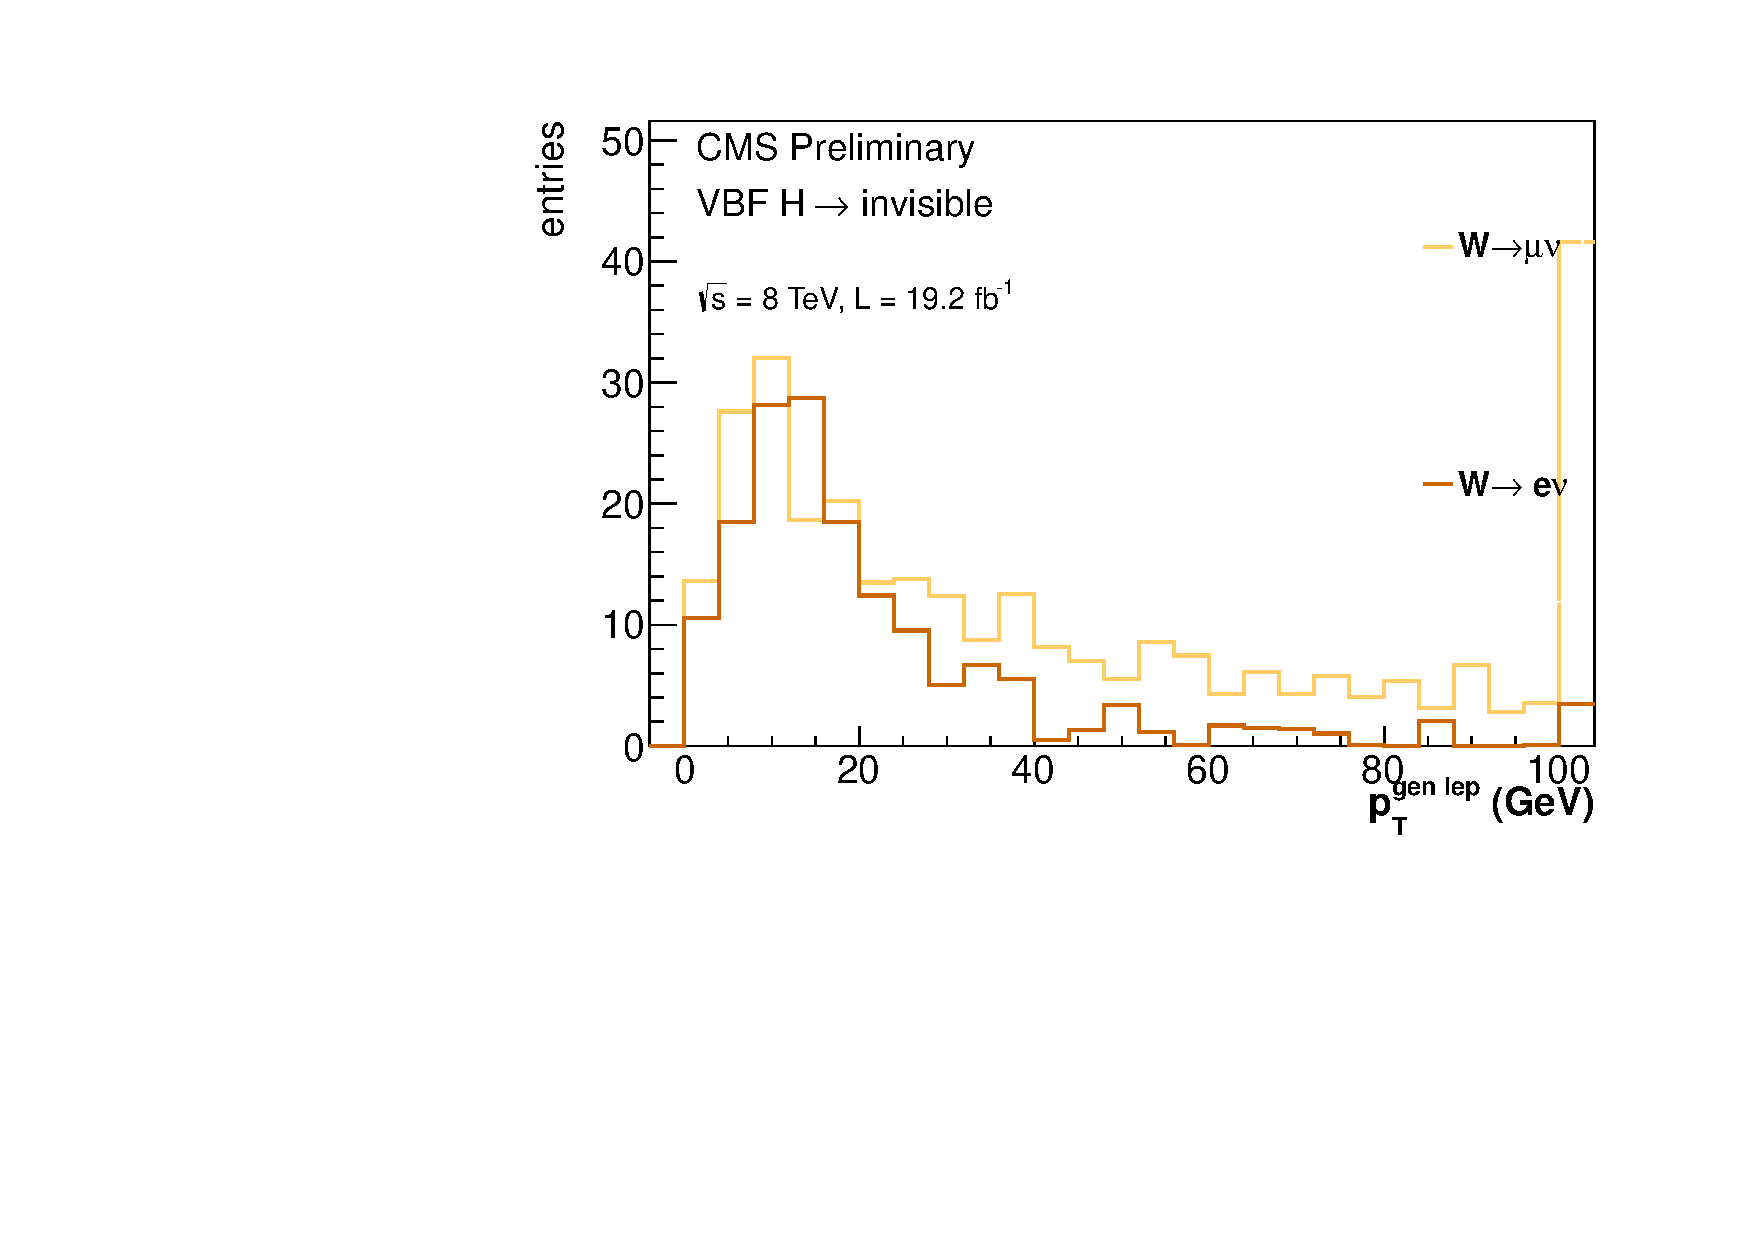
\includegraphics[width=.65\largefigwidth]{plots/parked/AN-14-243-figs/genlepstudy/outsideaccloosedphi/nunu_genlep1_pt.pdf}}
  \caption{Distributions of the number of jets with \pt$>15$ \GeV (a), \jetmetdphi (b) and the \pt of the leading generator level electron/muon (c) in $\PW\rightarrow e/\mu\nu$ events in a region with cuts which are the same as those of the signal region except that the \jetmetdphi requirement has been loosened to 1 and a generator level lepton outside the detector acceptance for both electrons and muons is required. The last bin of each distribution contains the events above the range displayed.}
  \label{fig:enumunudiff}
\end{figure}

\subsection{Z$\rightarrow \nu\nu$+jets}
\label{sec:parkedznunu}
%same as before studies of uncertainty with madgraph and mcfm
The irreducible $\PZ\rightarrow\nu\nu$ background is estimated using a very similar method to that used in the prompt analysis (\SectionRef{sec:promptznunu}). A reminder of the method highlighting the differences from the prompt analysis is given here.

The method starts by defining a dimuon control region by taking the signal region requirements and replacing the muon veto with the requirement that there are two tight muons with invariant mass compatible with a \PZ boson, i.e. between 60 and 120 \GeV, and no other muons in the event. The number of events in this dimuon control region is then extrapolated to the signal region using efficiencies and cross-section ratios calculated using \ac{MC} events. As in the prompt analysis a \Zmumu \ac{MC} sample with the reconstructed leptons ignored and a requirement that there is a generator level dimuon system with invariant mass between 80 and 100 \GeV (i.e. compatible with a \PZ boson) is used to estimate the contribution in the signal region from \Znunu processes. The mass window used here is tighter than that used to define the dimuon control region because the generator level lepton \pt resolution is better than that of reconstructed leptons. \Znunu \ac{MC} events are not used for this estimation due to the limited size of the available \Znunu \ac{MC} samples. Whilst the number of events in the dimuon control region is small the agreement between data and \ac{MC} is good as can be seen from \FigureRef{fig:parkedznunu}

\begin{figure}
  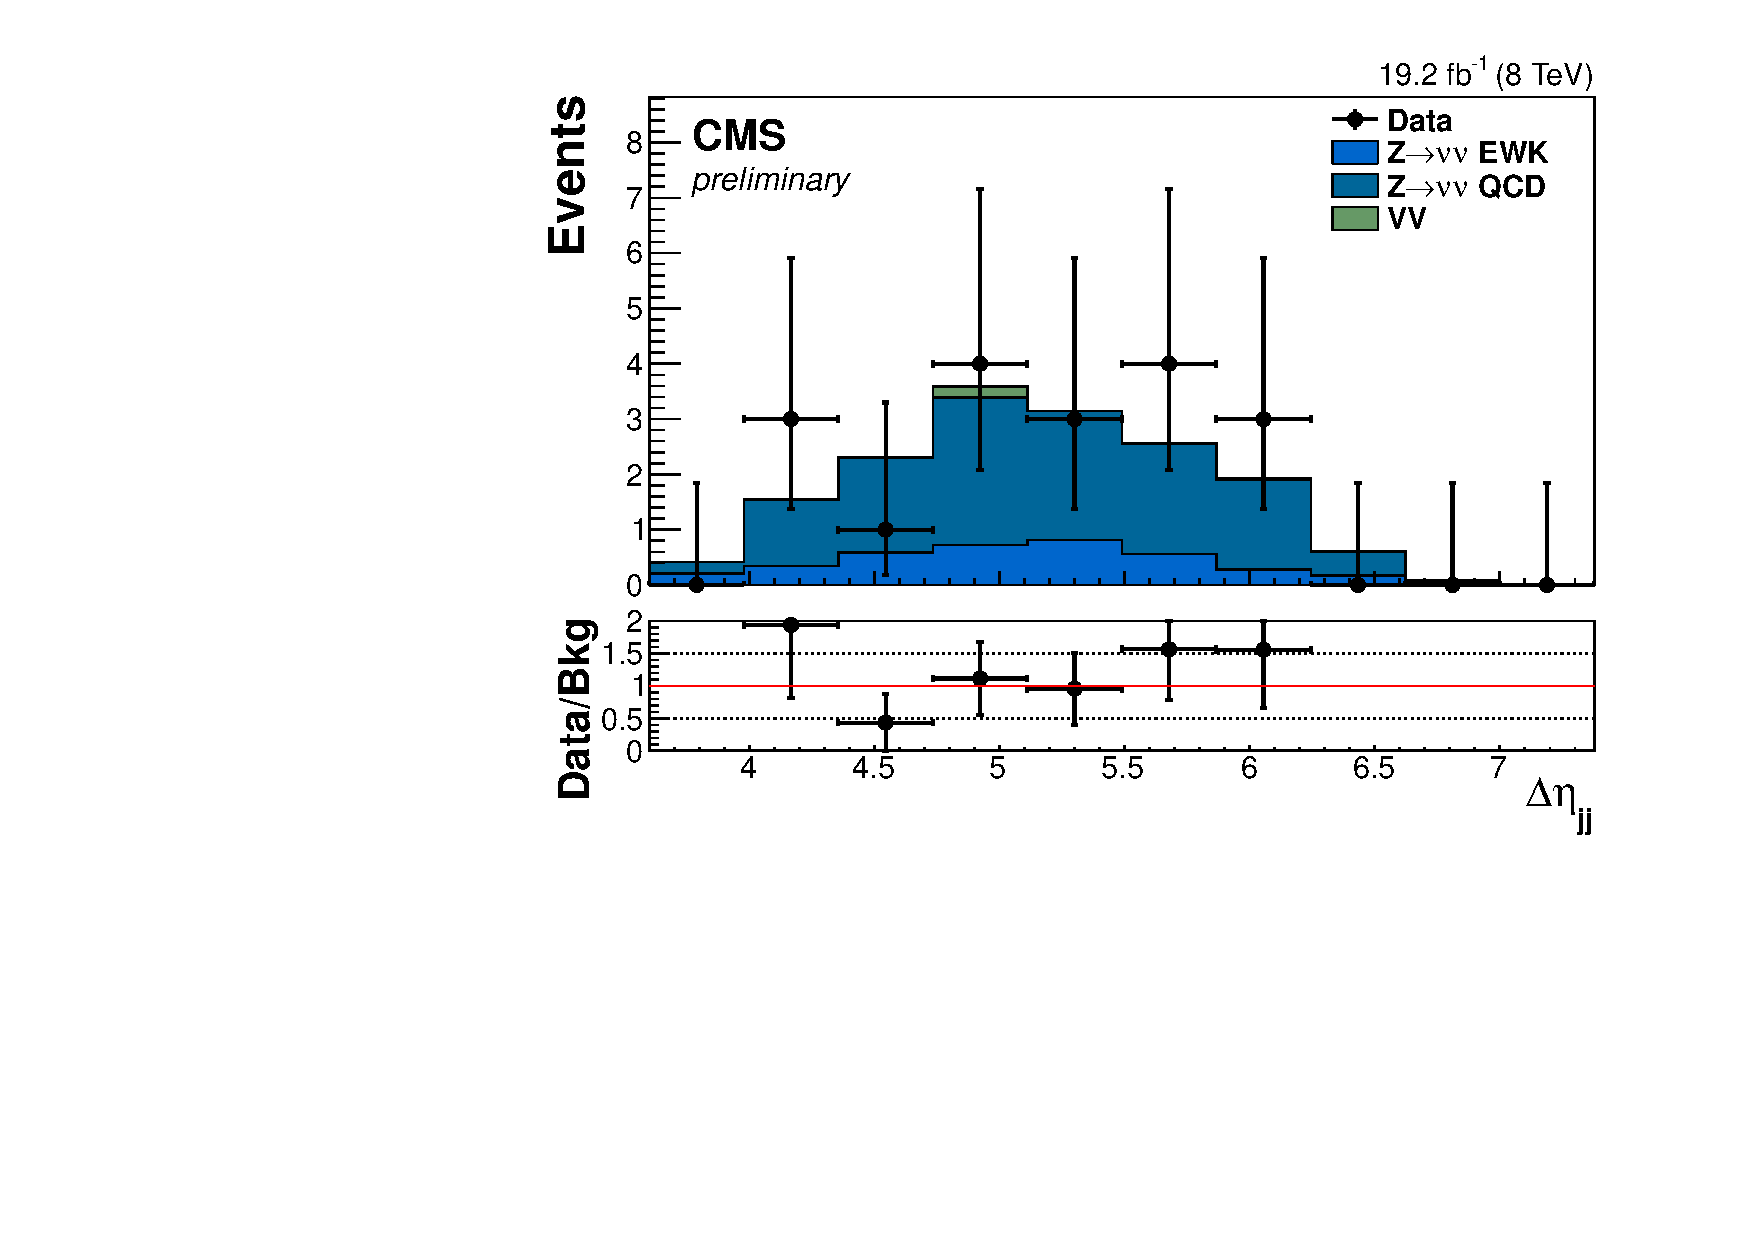
\includegraphics[width=.65\largefigwidth]{plots/parked/HIG-14-038-figs/output_sigreg/mumu_dijet_deta.pdf}
  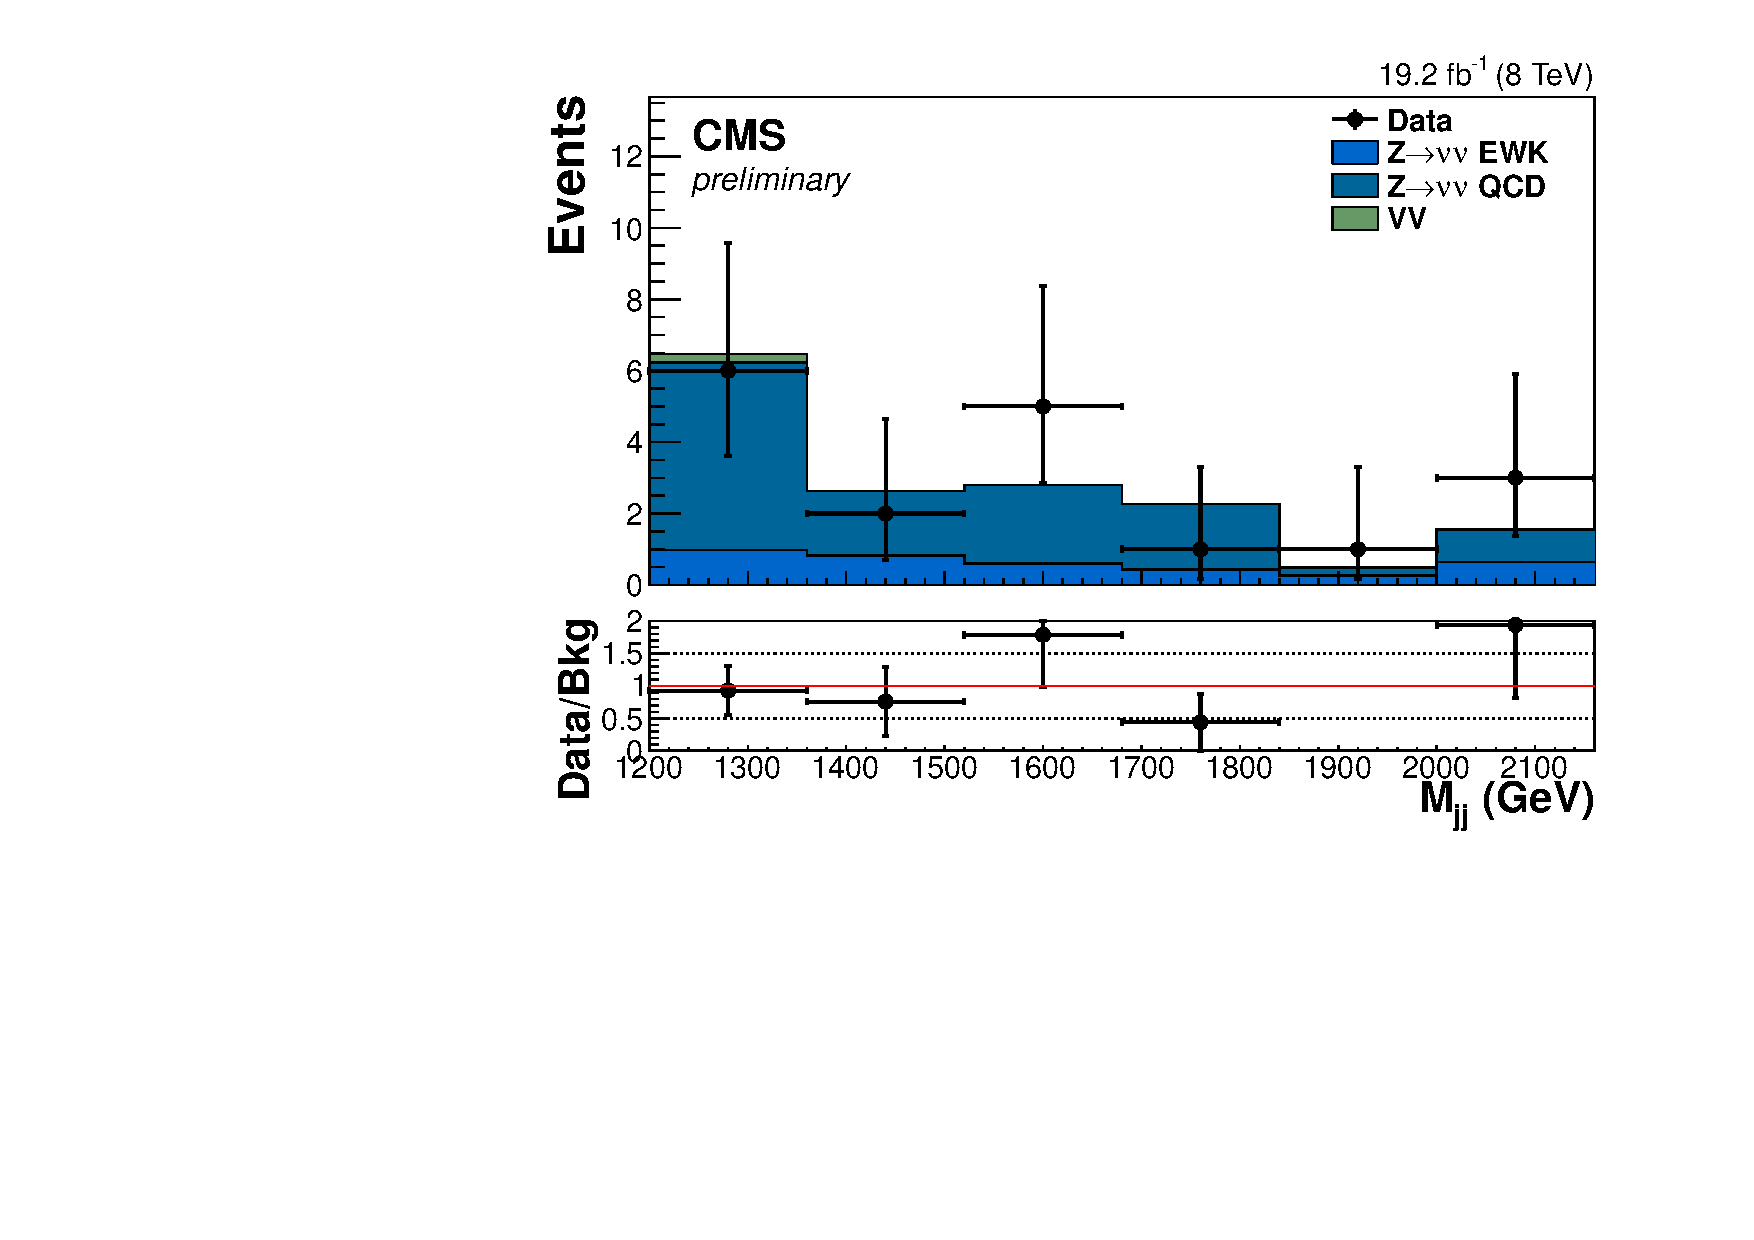
\includegraphics[width=.65\largefigwidth]{plots/parked/HIG-14-038-figs/output_sigreg/mumu_dijet_M.pdf}

  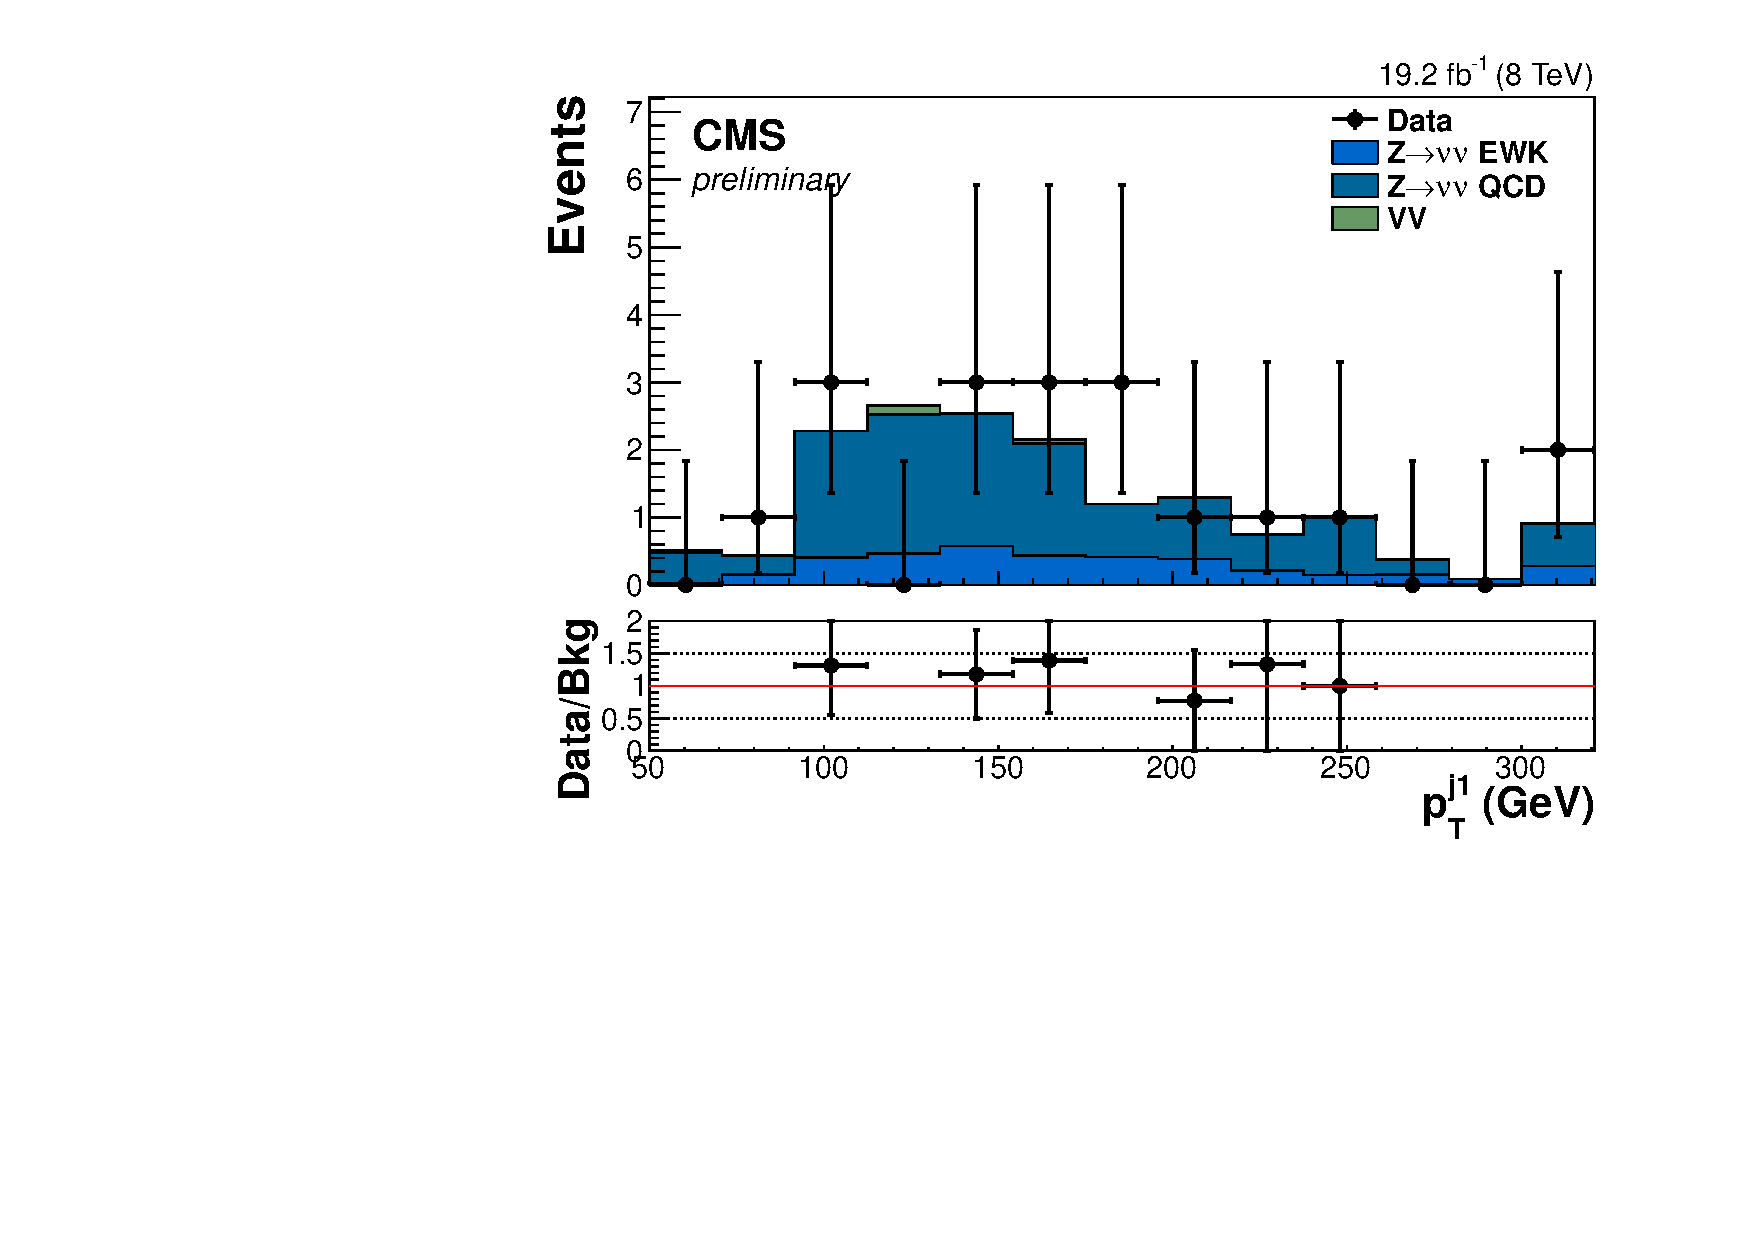
\includegraphics[width=.65\largefigwidth]{plots/parked/HIG-14-038-figs/output_sigreg/mumu_jet1_pt.pdf}
  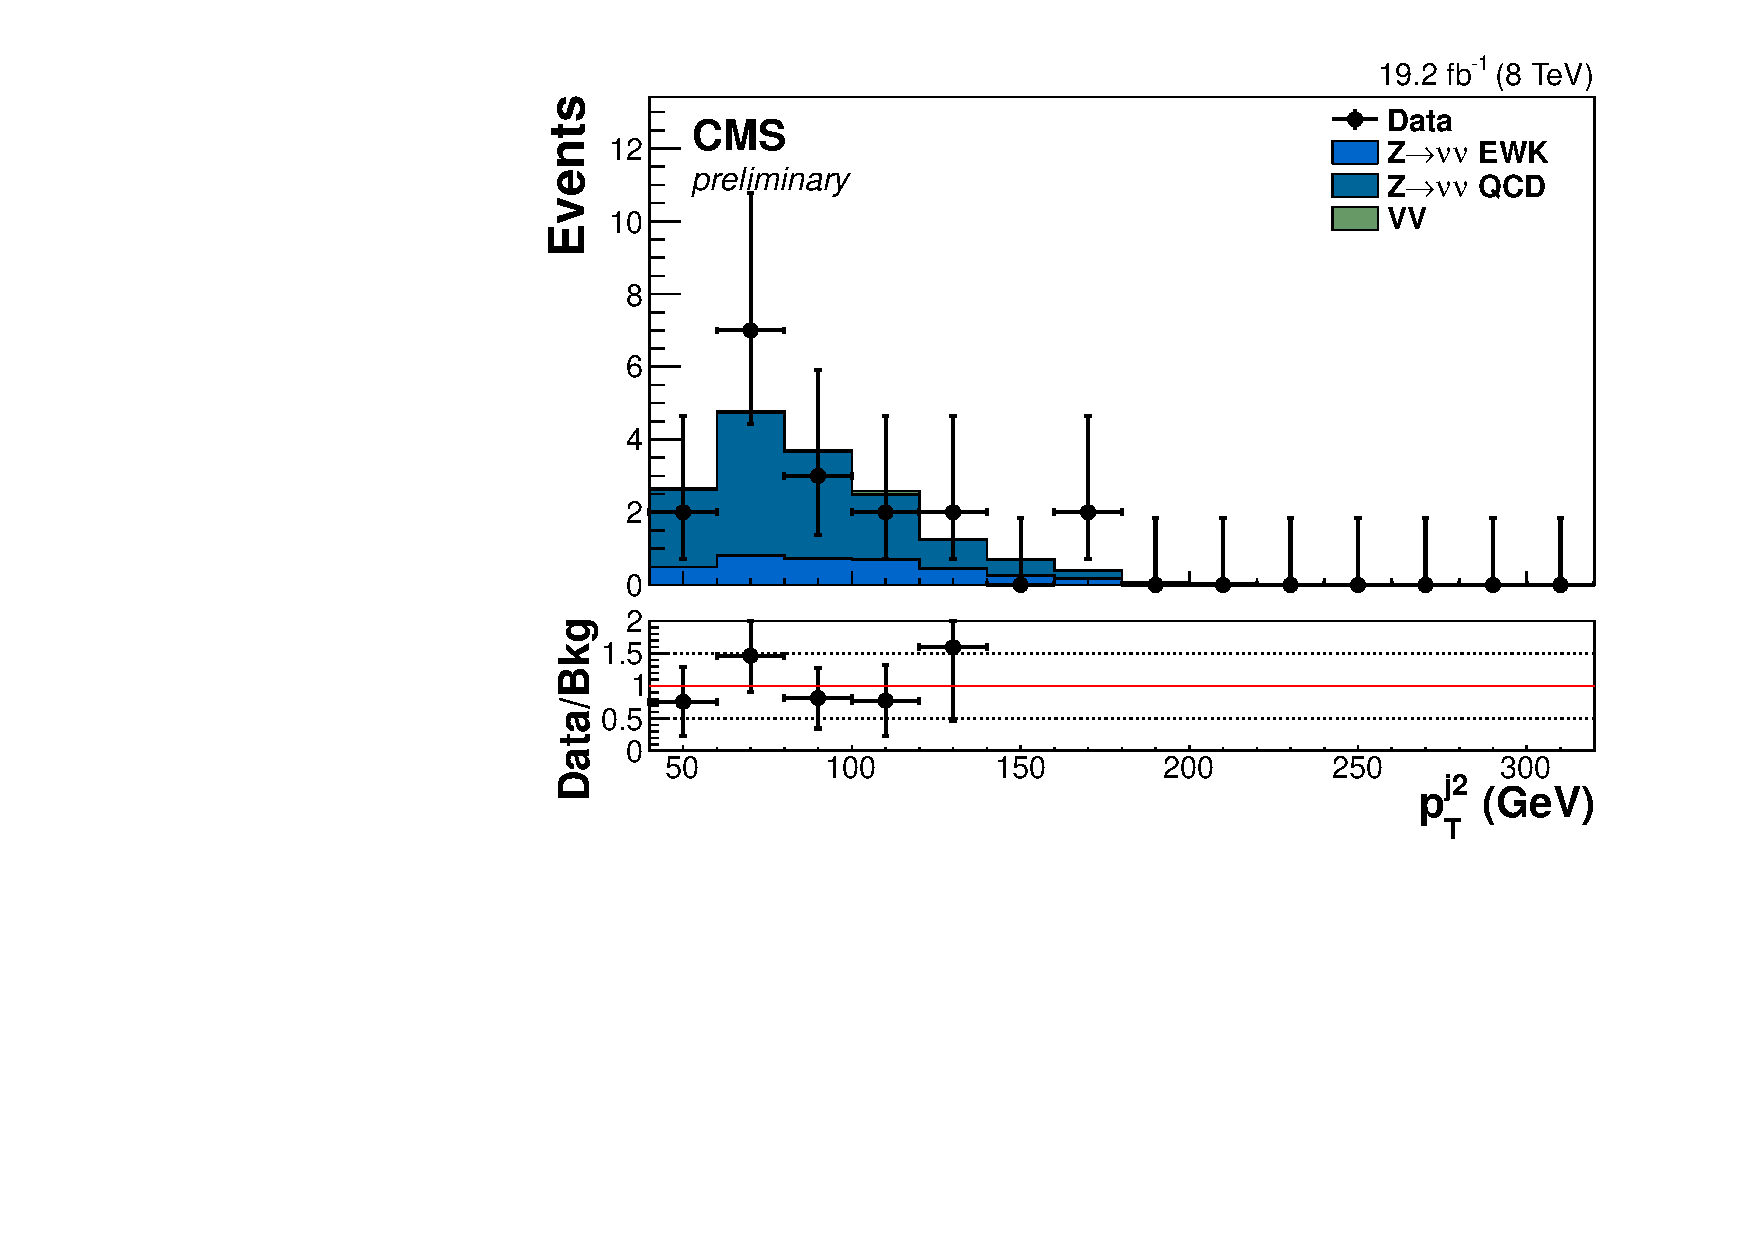
\includegraphics[width=.65\largefigwidth]{plots/parked/HIG-14-038-figs/output_sigreg/mumu_jet2_pt.pdf}

  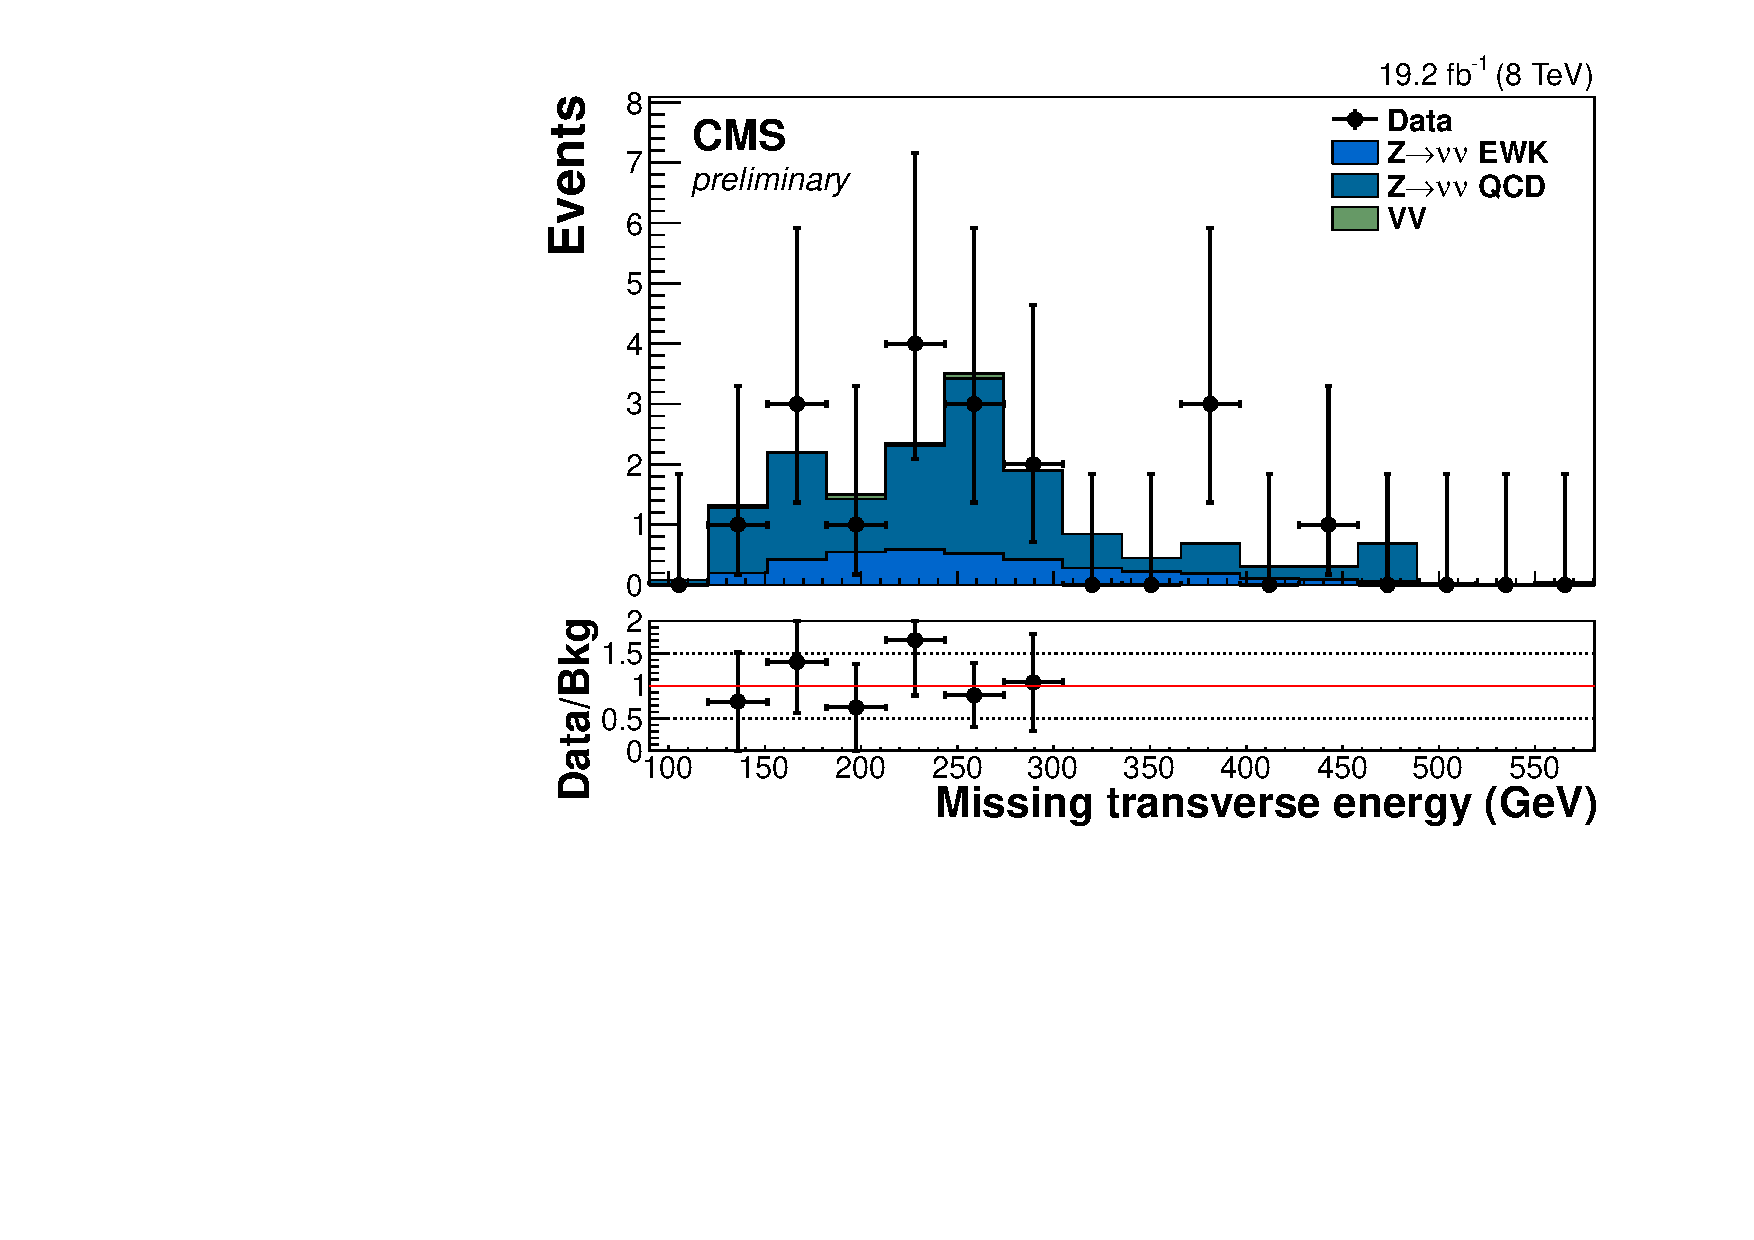
\includegraphics[width=.65\largefigwidth]{plots/parked/HIG-14-038-figs/output_sigreg/mumu_metnomuons.pdf}
  \includegraphics[width=.65\largefigwidth]{plots/parked/HIG-14-038-figs/output_sigreg/mumu_metnomu_significance.pdf}

  \includegraphics[width=.65\largefigwidth]{plots/parked/HIG-14-038-figs/output_sigreg/mumu_jetmetnomu_mindphi.pdf}
  \includegraphics[width=.65\largefigwidth]{plots/parked/HIG-14-038-figs/output_sigreg/mumu_m_mumu.pdf}
  \caption{Distributions of variables in data and \ac{MC} events in the dimuon control region. \ac{MC} events from V+jets backgrounds are scaled by their data-driven scale factors. The variables shown are from top to bottom and left to right \detajj, \Mjj, the leading and sub-leading jet's \pt, \METnoMU, \METsig, \jetmetdphileading and the invariant mass of the dimuon system. The contributions to this region from electroweak and \ac{QCD} produced $\PZ+$jets events are shown separately. The last bin of each distribution contains the events above the range displayed~\cite{CMS-PAS-HIG-14-038}.}
  \label{fig:parkedznunu}
\end{figure}

The formulae used to carry out the extrapolation from the control region to the signal region are given in Equation~\ref{eq:zdatabkg} which is repeated here for reference:
\begin{equation}
  \label{eq:zdatabkgrep}
  N^{S}_{Exp}=\left(N^{C}_{Data}-N^{C}_{Bkg}\right)\cdot\frac{\sigma\left(\PZ\rightarrow\nu\nu\right)}{\sigma\left(\PZ/\gamma^{*}\rightarrow\mu\mu\right)}\cdot\frac{\epsilon^{S}_{VBF}}{\epsilon^{C}_{VBF}},
\end{equation}
where $\epsilon^{S}$ and $\epsilon^{C}$ are calculated as in Equations~\ref{eq:zdataeffs} and \ref{eq:zdataeffc} repeated here:
\begin{align}
  \label{eq:zdataeffsrep}
  \epsilon^{S}_{VBF}&=\frac{ \sigma\left(\PZ\rightarrow\nu\nu,EWK\right) \frac{N^{S}_{MC}\left(EWK\right)} {N_{gen}\left(\PZ \rm{mass},EWK\right)} + \sigma\left(\PZ\rightarrow\nu\nu,QCD\right) \frac{N^{S}_{MC}\left(QCD\right)} {N_{gen}\left(\PZ \rm{mass},QCD\right)} } {\sigma\left(\PZ\rightarrow\nu\nu,EWK\right) + \sigma\left(\PZ\rightarrow\nu\nu,QCD\right)},\\
  \label{eq:zdataeffcrep}
  \epsilon^{C}_{VBF}&=\frac{  \sigma\left(\PZ/\gamma^{*}\rightarrow\mu\mu,EWK\right) \frac{N^{C}_{MC}\left(EWK\right)} {N_{gen}\left(EWK\right)} + \sigma\left(\PZ/\gamma^{*}\rightarrow\mu\mu,QCD\right) \frac{N^{S}_{MC}\left(QCD\right)} {N_{gen}\left(QCD\right)}  }{\sigma\left(\PZ/\gamma^{*}\rightarrow\mu\mu,EWK\right)+\sigma\left(\PZ/\gamma^{*}\rightarrow\mu\mu,QCD\right)}.
\end{align}
As the \Zmumu and \Znunu cross-sections are calculated before the analysis selection cuts and do not depend on detector calibration, the same values are used as in the prompt analysis shown in \TableRef{tab:promptznunueffs}. The other inputs to the above equations and the results of the estimation are shown in \TableRef{tab:parkedznunu}.

Although it is not used in the \Znunu background estimation method, the ratio between the number of \ac{MC} dimuon events, both from electroweak and \ac{QCD} events, and the number of data events minus expected backgrounds from other processes is shown for comparison with the data driven scale factors used in the $\PW+$jets background estimate. The ratio is, like those in the $\PW+$jets background estimation found to be significantly different from 1. 
%inputs where the same and where different from prompt

\begin{table}
  \caption{The inputs to Equations~\ref{eq:zdatabkgrep}, ~\ref{eq:zdataeffsrep} and ~\ref{eq:zdataeffcrep} and the final estimate of the \Znunu background in the signal region for the parked data analysis. Also shown for comparison is the ratio between the \ac{MC} prediction of the number of \Zmumu events in the control region and the number of data events in the control region. The systematic uncertainties quoted include MC statistical uncertainties and all sources listed in \SectionRef{sec:parkedsyst}. }
  \label{tab:parkedznunu}
  \begin{tabular}{lcc}
    \hline
    \hline
    $N_{gen}\left(\mathnormal{EWK}\right)$&\multicolumn{2}{c}{5781.9}\\
    $N_{gen}\left(\PZ\rm{mass},\mathnormal{EWK}\right)$&\multicolumn{2}{c}{4226.5}\\
    $N_{gen}\left(\mathnormal{QCD}\right)$&\multicolumn{2}{c}{22789000}\\
    $N_{gen}\left(\PZ\rm{mass},\mathnormal{QCD}\right)$&\multicolumn{2}{c}{20334000}\\
    \hline
    \hline
    & Signal region & Control region \\
    \hline
    \hline
    $N_{Data}$ & N/A & $18\pm 4.2\stat$ \\
    $N_{Bkg}$ & N/A & $0.2\pm 0.1 (\rm{MC\,stat})$ \\
    $N_{MC}\left(EWK\right)$ & $7.9\pm 0.2 (\rm{MC\,stat})$& $6.0\pm 0.2 (\rm{MC\,stat})$ \\
    $N_{MC}\left(QCD\right)$ & $29.5\pm 3.0 (\rm{MC\,stat})$ & $20.5\pm 2.5 (\rm{MC\,stat})$ \\
    \hline
    $\frac{N^{C}_{Data}-N^{C}_{Bkg}}{N^{C}_{MC}\left(EWK\right)+N^{C}_{MC}\left(QCD\right)}$ & \multicolumn{2}{c}{$0.67\pm 0.16\stat\pm 0.06 (\rm{MC\,stat})$} \\
    \hline
    $N_{\PZ\rightarrow \nu\nu/\PZ\rightarrow/\gamma^{*}\rightarrow\mu\mu}$ & $\textcolor{red}{158.1\pm 37.8\stat\pm 21.2\syst}$ & $17.8\pm 4.2\stat\pm 0.1 (\rm{MC\,stat})$ \\
    \hline
    \hline
  \end{tabular}
\end{table}

%studies of uncertainty on cross-section ratio
In the prompt analysis one of the largest uncertainties, being 44\% of the size of the total systematic uncertainty on the total background estimate, was the uncertainty on the ratio between the \Zmumu and \Znunu cross-sections in the \ac{VBF} phase space. To reduce this uncertainty in this analysis the cross-section ratio was calculated both with \textsc{MadGraph} and \textsc{aMC\@NLO\_MG5}. The \textsc{aMC\@NLO\_MG5} calculation was carried out by generating both \Zmumu and \Znunu events and calculating the ratio of the efficiencies of events in each sample to pass the analysis selection. The selection was applied to generator level objects, with jets being constructed using the algorithm described in \SectionRef{sec:jets} from the generator level quarks and gluons, and the \MET being taken to be the \PZ boson's \pt. For the \textsc{MadGraph} calculation, the same generator level selection was applied to the \Zmumu samples that are used in the background estimation method and the small available \Znunu sample and the same efficiency ratio was calculated. The prediction from \textsc{aMC\@NLO\_MG5} had a very large statistical uncertainty due to it being computationally prohibitive to generate a larger sample. However within the uncertainties the prediction is compatible with that from \textsc{MadGraph}. The uncertainty from \textsc{MadGraph} is already accounted for by the \ac{MC} statistical uncertainty on the prediction of the numbers of events in the \Zmumu sample no additional uncertainty was added to the analysis.

%taken from AN
\subsection{V+jets consistency tests}
\label{sec:parkedclosure}
%as in AN relatively good agreement but large uncertainties
To check the consistency of the scale factors obtained from the different V+jets background estimation methods, a study was undertaken to use the single muon control region scale factor to predict the data yield in the other control regions. Rather than calculate a single scale factor for the control region, as was done in the background estimation methods, scale factors were calculated for each bin of the distribution of several variables. These scale factors were then applied to the \ac{MC} estimate in the corresponding bin of the other control regions, allowing the behaviour of the scale factor as a function of the variable to be seen. The resulting estimate was compared to the data yield minus the background expected from other processes from \ac{MC}.

The scale factor weighted \ac{MC} was found to agree better with data than the unweighted \ac{MC}, with the differences seen between the weighted \ac{MC} and the data being less than systematic uncertainty in the majority of bins, which gives confidence that the data driven methods improve the background estimations. The results of these studies in the \METnoMU distribution can be seen in \FigureRef{fig:parkedclosure}.
\begin{figure}
  \subfloat[]{\includegraphics[width=.65\largefigwidth]{plots/parked/AN-14-243-figs/closuretests/closuremetnomuonsWJets_enu.pdf}}
  \subfloat[]{\includegraphics[width=.65\largefigwidth]{plots/parked/AN-14-243-figs/closuretests/closuremetnomuonsWJets_taunu.pdf}}

  \subfloat[]{\includegraphics[width=.65\largefigwidth]{plots/parked/AN-14-243-figs/closuretests/closuremetnomuonsZJets_ll_all.pdf}}
  \caption{The distribution of \METnoMU expected in the single electron (a), single tau (b) and dimuon control regions (c) from \ac{MC} (red), data minus other background processes (blue) and \ac{MC} weighted by the data driven scale factor calculated for each bin of the \METnoMU distribution in the single muon control region as described in \SectionRef{sec:parkedclosure} (green). The lower plot shows the ratio between the data driven scale factor weighted \ac{MC} and the data minus other background processes. The grey band on the lower plots represents the systematic uncertainty from all sources described in \SectionRef{sec:parkedsyst}.}
  \label{fig:parkedclosure}
\end{figure}

\subsection{V+jets scale factor investigations}
\label{sec:parkedscalefactors}
The data driven scale factors seen in the V+jets background estimation methods are consistently significantly different from 1. To investigate the reason for this difference the variation of the scale factors as a function of the analysis selection criteria was studied. Due to the high thresholds of the triggers with which the parked data were collected, it was necessary to use a different trigger for this study. The particular trigger chosen was the same single muon trigger used for the trigger efficiency measurements described in \SectionRef{sec:parkedtrigger}. The study was therefore restricted to the single muon control region as it has muons present and contains significantly more events than the dimuon control region. To ensure that the trigger was fully efficient the muon \pt cut was tightened to 25 \GeV.

The requirements on the leading and sub-leading jet's \pt, \Mjj, \jetmetdphi, \METnoMU and \METsig were then varied to ascertain which requirements caused the largest variations in the scale factor. The \METnoMU and leading jet \pt requirements were found to have no discernible effect on the scale factor. The effects from the sub-leading jet \pt and \METsig requirements were found to be less than 5\%. By contrast, the \jetmetdphi and \Mjj requirements were found to significantly alter the scale factor obtained. As can be seen in \FigureRef{fig:jetmetdphimjjscalefactor}a, when these two requirements are loosened the scale factor increases significantly.

\begin{figure}
  \subfloat[]{\includegraphics[width=.65\largefigwidth,height=.3\textheight]{plots/parked/AN-14-243-figs/jetmetdphimjj.pdf}}
  \hspace{.1cm}
  \subfloat[]{\includegraphics[width=.65\largefigwidth,height=.3\textheight]{plots/parked/AN-14-243-figs/dphijjmjj.pdf}}
  \caption{The data driven scale factor obtained from a single muon control region, as described in \SectionRef{sec:parkedscalefactors}, as a function of the cuts on \jetmetdphi and \Mjj (a) and $\Delta\phi_{jj}$ and \Mjj (b). It is important to note that the requirement on $\Delta\phi_{jj}$ is that the event have a value lower than the cut threshold, so the requirement is tighter to the left of the plot. The parked data analysis preselection requirements correspond to the top right bin of (a).}
  \label{fig:jetmetdphimjjscalefactor}
\end{figure}

%study of dphijj
To determine whether the scale factor depends more strongly on the jet or \METnoMU azimuthal angle the requirement on \jetmetdphi was replaced with a requirement on the difference in azimuthal angle between the two tag jets, $\Delta\phi_{jj}$, which doesn't depend on the \METnoMU and the study was repeated. As can be seen in \FigureRef{fig:jetmetdphimjjscalefactor}b, the scale factor was still found to vary in the same range with $\Delta\phi_{jj}$, indicating that the use of the \METnoMU azimuthal angle does not cause a further deviation from 1 than that present already due to jet related effects.

The looser the requirements on the jet kinematics are the closer the scale factor is to 1. It therefore seems that the deviation in the scale factor from 1 is caused by mismodelling of the jet related variables in V+jets \ac{MC}. The distributions of variables for events in the various control regions shown in Figures~\ref{fig:parkedwenu}-\ref{fig:parkedznunu} show good shape agreement between data and \ac{MC}, indicating that the shape in these regions is not significantly mismodelled. Also, the data driven methods used to estimate the V+jets background correct for the overall normalisation difference from mismodelling in areas of phase space outside the analysis control and signal regions. For these two reasons this mismodelling is not expected to cause problems for the analysis.

\subsection{QCD}
\label{sec:parkedQCD}
%describe QCD MC, problem with real and fake met
As mentioned in \SectionRef{sec:parkedsel} events from \ac{QCD} multijet processes are very difficult to model using \ac{MC}, as their high production cross-section and low probability to pass the selection cuts makes the number of events which must be generated prohibitively large. In an attempt to circumvent this problem a dedicated sample of \ac{QCD} multijet events with \ac{VBF}-like cuts imposed at generator level was produced. Specifically, the \MET was required to be greater than 40 \GeV, at least 2 jets with \pt$>20$ within the detector acceptance had to be present, and at least one pair of those jets was then required to have \Mjj$>700$ \GeV and $\detajj>3.2$. As can be seen from \FigureRef{fig:parkedpresel} this sample does not adequately describe the events passing the trigger selection.

\begin{figure}
  \includegraphics[width=.7\largefigwidth]{plots/parked/AN-14-243-figs/Joao_140209_p11.png}
  \caption{The reconstructed \MET, PFMET, as a function of the generator level \MET, genMET in a \ac{MC} sample with no generator level cuts on \MET or jet kinematics. For reference, the cut placed on genMET in the dedicated \ac{VBF} \ac{QCD} multijet sample is shown in red, and the offline prompt analysis cut on PFMET is shown in blue~\cite{ARTICLE:CMSAN-14-243}.}
  \label{fig:parkedmcqcd}
\end{figure}

To investigate where this mismodelling comes from the reconstructed \MET was plotted as a function of the generator level \MET in the \ac{QCD} multijet \ac{MC} sample centrally produced by CMS as shown in \FigureRef{fig:parkedmcqcd}. This sample does not have any generator level cuts on the \MET or jet kinematics. Most events fall in the bottom left of this plot, having low \MET at both generator level and offline. These events would therefore not enter the analysis signal region and would also be rejected by the generator level cut as intended. There is then another class of events distributed around the diagonal of the plot due to the \MET resolution, with higher values of both generator level and offline \MET. These on-diagonal events would be expected to be well modelled by the \ac{VBF} \ac{QCD} sample as most of them which fall into the analysis signal region, which requires \MET$>90$ \GeV, would be expected to pass the generator level cut. Finally, there is a third type of events, which have low values of generator level \MET, but high values of offline \MET due to mismeasurement. These so-called ``fake'' \MET events are believed to be the cause of the \ac{VBF} \ac{QCD} sample not adequately modelling the \ac{QCD} background in this analysis, as they will be removed by the generator level cut, but will be present in the analysis signal region. 

%as in PAS use isolated non-isolated met analogy with other methods
%data driven method therefore necessary explain as in pas
It can be seen from the location of the gaps between the data and \ac{MC} predictions in \FigureRef{fig:parkedpresel} that the fake \MET events, like the well modelled on-diagonal events, have at least one jet close in $\phi$ to the \MET, and have low values of \METsig. They are therefore expected to be almost entirely removed by the analysis selection. Nevertheless it is important to provide an estimate of the small remaining number of \ac{QCD} background events of both types. Due to the difficulties with \ac{MC} estimates outlined above this estimation must be data driven.

%why not ABCD, then follow PAS
The ABCD method used in the prompt analysis cannot be used for this analysis because the regions where only one of the two main anti-\ac{QCD} cuts is inverted are expected to have non-negligible signal contributions (approximately 10\% of the total number of data events assuming a 125 \GeV Higgs boson decaying entirely to invisible final states). An alternative method using events with ``non-isolated'' \MET, i.e. that with a jet close to it in $\phi$, is therefore used. This non-isolated method involves three regions: (i) the ``inverted'' region where the shape of the distributions of key variables for the \ac{QCD} background is determined, (ii) the ``3-jet'' region where this shape is validated, and (iii) a set of ``sideband'' regions where a normalisation for the \ac{QCD} shape is extracted. A schematic of these regions is shown in \FigureRef{fig:parkedqcdregions}

\begin{figure}[h!]
\begin{center}
  \begin{tabular}{c r}
    &   \\
    \multirow{4}{*}{$\mathrm{min}\Delta\phi(\MET,\mathrm{j1/j2})$} & \\
    & \multirow{2}{*}{2.3} \\
    &  \\
    & \multirow{2}{*}{2.0}  \\
    & \\
    & \multirow{2}{*}{1.0}\\
    \multirow{2}{*}{$\mathrm{min}\Delta\phi(\MET,\mathrm{all jets})$} & \\
    & \multirow{2}{*}{0.0}\\
    & \\
    & \\
  \end{tabular}
  \begin{tabular}{c c c | c c c c}
\multicolumn{7}{|c}{}\\
\multicolumn{3}{|c|}{{\cellcolor{cyan}}} & \multicolumn{3}{|c}{\cellcolor{green}} & \\
\multicolumn{3}{|c|}{{\cellcolor{cyan}}} & \multicolumn{3}{|c}{\multirow{-2}{*}{\cellcolor{green}Signal}}  & \multirow{4}{*}{} \\
\cline{4-7}
\multicolumn{3}{|c|}{\multirow{-2}{*}{{\cellcolor{cyan}} Sideband 2}} & \multicolumn{3}{|c}{} & \\
\multicolumn{3}{|c|}{\multirow{-2}{*}{{\cellcolor{cyan}}}} & \multicolumn{3}{|c}{} & \\
\hline
\multicolumn{3}{|c|}{{\cellcolor{cyan}}} & \multicolumn{3}{|c}{\cellcolor{cyan}} & \\
\multicolumn{3}{|c|}{\multirow{-2}{*}{{\cellcolor{cyan}}Sideband 1}} & \multicolumn{3}{|c}{\multirow{-2}{*}{\cellcolor{cyan}Sideband 3}} & \\
\hline
\hline
\multicolumn{3}{|c|}{} & \multicolumn{3}{|c}{\cellcolor{orange}} & \\
\multicolumn{3}{|c|}{} & \multicolumn{3}{|c}{\multirow{-2}{*}{\cellcolor{orange}Inverted}} & \multirow{-2}{*}{} \\
\hline
\multicolumn{2}{l}{\hspace{-.4cm}3.0}  & \multicolumn{2}{c}{\hspace{.9cm}4.0} &  & \multicolumn{2}{c}{} \\
\multicolumn{6}{c}{MET significance} & \\
\end{tabular}
\end{center}
\caption{A schematic of the regions used in the \ac{QCD} background estimation.}
\label{fig:parkedqcdregions}
\end{figure}


The contribution from V+jets backgrounds in these regions is estimated using \ac{MC} normalised with the data driven method described by \EquationRef{eq:wdatabkgrep}. The control regions used for each background in each region are defined by making the same modifications to the region that were made to the signal region to define the V+jets control regions used in Sections~\ref{sec:parkedwenu}-\ref{sec:parkedznunu}.

%inverted
The inverted region is defined starting from the signal region, by swapping the \jetmetdphi$>2.3$ requirement for a requirement that only \jetmetdphileading is greater than 2.3, and then requiring that \jetmetdphi is less than 1. The resulting region consists of events with two signal-like jets, well separated from the \MET, but also an additional jet close to the \MET making it non-isolated.   As can be seen from \FigureRef{fig:parkeddataqcd}a the inverted region is dominated by \ac{QCD} events with only 20\% of the events expected to come from V+jets and other background processes. The \ac{QCD} shape is taken to be the shape of the data after subtracting the estimated contribution from all other background processes.


%3 jet
To ensure the \ac{QCD} shape derived from non-isolated \MET is adequate to describe the \ac{QCD} background with isolated \MET in the signal region the 3-jet region is used. This region is defined starting from the signal region by relaxing the \jetmetdphi and \METsig requirements from greater than 2.3 to greater than 1 and from greater than 4 to greater than 3 respectively, then requiring that there are at least three jets with \pt$>30$ \GeV in the event. The \ac{QCD} shape obtained from the inverted region is then normalised to the data yield minus the expected contribution from other backgrounds in this 3-jet region and plotted as a function of several variables. Good agreement between data and \ac{MC} is seen and the distribution of \METsig is shown in \FigureRef{fig:parkeddataqcd}b. 

\begin{figure}
  \subfloat[]{\includegraphics[width=.65\largefigwidth]{plots/parked/HIG-14-038-figs/output_invqcd_qcd_metnomu_significance.pdf}}
  \subfloat[]{\includegraphics[width=.65\largefigwidth]{plots/parked/AN-14-243-figs/output_invqcd_3j/nunu_metnomu_significance.pdf}}
  \caption{The distribution of \METsig in the inverted (a) and 3-jet (b) regions used in the \ac{QCD} background estimation. In (a) the \ac{QCD} shape is estimated using the \ac{VBF} \ac{QCD} sample, and in (b) the \ac{QCD} shape is taken from the inverted region as described in the text. Both shapes are normalised to the total number of events seen in the region minus the expected contribution from other backgrounds~\cite{CMS-PAS-HIG-14-038}.}
  \label{fig:parkeddataqcd}
\end{figure}

%sideband
To obtain the \ac{QCD} normalisation in the signal region several sideband regions were investigated. As has been described above the regions obtained by inverting the requirement on one of the two main anti-\ac{QCD} discriminant variables, \jetmetdphi and \METsig, have non-negligible signal contributions. However by inverting the requirements on both variables a \ac{QCD} dominated sideband can be obtained. This region is called ``sideband 1'' and the specific differences from the signal region are that we require $3<\METsig<4$ and $1<\jetmetdphileading<2$.  

Whilst the regions obtained from inverting only one of the \jetmetdphi or \METsig requirements have signal contributions of approximately 10\% for a \ac{SM} produced 125 \GeV Higgs boson with \BRinv$=100\%$, an invisible branching fraction of 100\% has already been ruled out so the actual signal contribution in these regions is expected to be smaller. Therefore, two further sideband regions which are not used in the final estimate, but which are used to validate the method are defined. Sideband 2 is the same as sideband 1, except that we require \jetmetdphileading$>2$. Sideband 3 is the same as sideband 1, except that we require \METsig$>4$. 



Scale factors were then obtained in each of the sideband regions by evaluating the following formula:
\begin{equation}
  SF=\frac{N_{Data}-N_{Bkg}}{N_{QCD}},
  \label{eq:parkedqcdscalefactor}
\end{equation}
where $N_{Data}$ and $N_{Bkg}$ ($N_{QCD}$) are (is)  evaluated using events passing the cuts of the particular sideband region being studied and also having \jetmetdphi$>1$ (\jetmetdphi$<1$). The scale factor was found to be much lower in sidebands 2 and 3 than in sideband 1. Signal events being present in sideband 2 or 3 would be expected to give larger and not smaller values of the scale factor, so signal contamination is not thought to be a concern. Therefore, the scale factor was studied as a function of the requirements on \jetmetdphileading and \METsig by gradually tightening the requirement on each variable in sideband 1 separately and recalculating the scale factor. The value of the scale factor as a function of the requirement placed on both \jetmetdphileading and \METsig can be seen in \FigureRef{fig:parkedqcdsfvar}.


\begin{figure}
  \subfloat[]{\includegraphics[clip=true,trim=0 0 0 180,width=\largefigwidth]{plots/parked/AN-14-243-figs/qcdEstimate/jetmetnomu_mindphi_norm1_SF.pdf}}

  \subfloat[]{\includegraphics[clip=true,trim=0 0 0 180,width=\largefigwidth]{plots/parked/AN-14-243-figs/qcdEstimate/metnomu_significance_norm1_SF.pdf}}
  \caption{The \ac{QCD} scale factor obtained in sideband 1 as a function of the lower bound on \jetmetdphi (a) and \METsig (b). Exponential fits which are used to extrapolate to higher values of these requirements are overlaid on both distributions, and the values of these fits at several representative values are displayed.}
  \label{fig:parkedqcdsfvar}
\end{figure}

The behaviour of the scale factor with each variable is compatible with both an exponential or linear decrease. So as to not underestimate the number of events from \ac{QCD} an exponential function, which yields slightly larger scale factors than a linear function, was fit to the distributions shown in \FigureRef{fig:parkedqcdsfvar}. Both these exponentials were then extrapolated to the signal region requirements. The average of these two extrapolations was used as the central prediction of the scale factor, and the envelope of their uncertainties was used to assign a systematic uncertainty. The final value of the scale factor is $0.048\pm 0.040$. The inverted region contains $363\pm 36$ events, so the total number of events expected from \ac{QCD} in the signal region is $17\pm 14$.

It should be noted that the \jetmetdphileading variable is not exactly the same as the \jetmetdphi used for the signal region selection. This alternate variable was used as cutting on \jetmetdphi left no \ac{QCD} events for the higher values of the requirement studied in \FigureRef{fig:parkedqcdsfvar}a. However, because the \jetmetdphi variable is more discriminating against \ac{QCD} than \jetmetdphileading the estimate presented above acts as an upper bound, which is acceptable given the low number of events ($<5\%$ of the total expected background) and its large relative uncertainty. Furthermore, the expected limit for the analysis is found to vary by less than 1\% on doubling or halving both the central value of the \ac{QCD} estimate and its uncertainty.


\subsection{Minor backgrounds}
\label{sec:parkedminor}
%straight from MC same XSec measurements as prompt
As in the prompt analysis, due to it being very small, the contribution to the signal and control regions from diboson and \Zmumu background processes was estimated from \ac{MC}. \textsc{Pythia 6} was used to generate diboson events, while \Zmumu events were generated with \textsc{MadGraph}. The \ac{MC} estimate of the diboson backgrounds was normalised using the most accurate CMS measurement at the time of this analysis~\cite{Chatrchyan2013190}. The expected number of events in the signal region from minor background processes is $3.9\pm 0.7$.

\section{Systematic uncertainties}
\label{sec:parkedsyst}
Most systematic uncertainties are calculated using the same methods as in the prompt analysis (see \SectionRef{sec:promptsyst}). The changes to the calculation of systematic errors on the top, $\PW\rightarrow\tau\nu$, $\PZ\rightarrow\nu\nu$ and \ac{QCD} multijet backgrounds have already been discussed in Sections \ref{sec:parkedtop}, \ref{sec:parkedwtaunu}, \ref{sec:parkedznunu} and \ref{sec:parkedQCD} respectively.

Despite the methods used being similar, in several cases the inputs to the methods have been updated to take into account improved measurements of various parameters using the full Run 1 dataset which were not available at the time of the prompt analysis. For example, the impacts of the \ac{JES}, \ac{JER} and \ac{UES} uncertainties are still estimated by recalculating the \pt of all jets and the \MET after varying each parameter up and down by one standard deviation and reperforming the analysis. However, the total uncertainty from these is smaller, being 6\% of the total expected background yield for this analysis where it was 7\% in the prompt analysis.

In addition to these changes a study was undertaken to estimate the impact of the trigger efficiency measurement uncertainties on the expected limit. As described in \SectionRef{sec:parkedtrigger}, all \ac{MC} events are reweighted by the measured trigger efficiency as a function of the events sub-leading jet \pt, \METnoMU and \Mjj. The uncertainty due to the reweighting process cancels in all data driven background estimates, as a ratio of \ac{MC} event yields is taken. To estimate the size of the uncertainty that should be applied to processes not estimated with data driven methods, the bin with the largest uncertainties on its fit for each era was chosen. It was then assumed that all bins had this worst-case uncertainty. This assumption resulted in a 2.3\% uncertainty on these non-data driven processes. Given that this error is smaller than many of the other errors considered, and that the uncertainty on the efficiency in most of the fit bins is significantly lower than this worst case, this uncertainty was considered negligible.

The fractional uncertainties on the total signal and background estimates from each source of uncertainty considered are shown in \TableRef{tab:parkedsyst} in decreasing order of the size of the uncertainty on the total background yield. It can be seen that the dominant uncertainties are statistical, with these being dominated by the low number of data events in the double muon control region (see \TableRef{tab:parkedznunu}).

\begin{table}
  \caption{A summary of the uncertainties on the total background and signal yields. All uncertainties affect the normalization of the yield, and are quoted as the change in \% in the total background or signal estimate, when each systematic effect is varied according to its uncertainties. The signal uncertainties are given for $m_{H}=125$\GeV and $\BRinv=100$\%.}
  \label{tab:parkedsyst}
  \begin{tabular}{lcc}
    \hline \hline
    Source  & Total background & Signal     \\
    \hline
    Control region statistics & 9.3 & - \\
    MC statistics & 5.4 & 3.8 \\
    \ac{JES} & 4.6 & 11 \\
    $\PW\rightarrow\tau\nu$ control region extrapolation & 4.3 & - \\
    QCD background estimation & 3.2 & - \\
    \ac{JER} & 3.0 & 1.8 \\
    Lepton ID efficiency & 2.4 & - \\
    \ac{UES} & 1.9 & 1.6 \\
    Pileup weight & 1.1 & 1.5 \\
    Top MC scale factor unc. & 0.25 & - \\
    Luminosity & 0.02 & 2.6 \\
    QCD scale, PDF and cross-section uncertainties & 0.01 & 5.2 \\
    \hline
    Total & 13.6 & 13.3 \\
    \hline \hline
  \end{tabular}
\end{table}



%Maybe explain uncertainty impact calculations and pulls test and give order of importance of nuisances state no issues found with pulls. possibly move pulls to combinations

\section{Results}                                                                                                                                        
\label{sec:parkedresults}
The final predicted yields for each background process are shown, along with their uncertainties in \TableRef{tab:parkedresults}. The total predicted event yield from background processes is $439.4\pm 40.7\stat\pm 43.5 \syst$. Assuming an \ac{SM} produced Higgs boson which decays 100\% of the time to invisible final states, $296.2\pm 39.4\syst$ events from signal processes are expected. 508 events are observed, which is slightly more than one standard deviation above the background only prediction. The distributions of the variables in the signal region used in the analysis selection are shown in \FigureRef{fig:parkednunucontplots}. The shapes of these distributions for data and the predicted backgrounds agree well, giving further evidence that the excess of events is not significant.

%yields etc table
\begin{table}
  \caption{The estimated numbers of background and signal events from each process, together with the observed yield, in the signal region. The signal yield assumes a Higgs boson mass of 125 \GeV and \BRinv$=100\%$. Where two errors are quoted they are the statistical and systematic uncertainties respectively, where only one is quoted it is the systematic uncertainty.}
  \label{tab:parkedresults}
  \begin{tabular}{lc}
    \hline \hline
    Process & Event yields \\
    \hline
    $Z\rightarrow\nu\nu$&$158.1 \pm 37.3 \pm 21.2$\\
    $W\rightarrow e\nu$&$57.9 \pm 7.4 \pm 7.7$\\
    $W\rightarrow\mu\nu$&$102.5 \pm 6.2 \pm 11.7$\\
    $W\rightarrow\tau\nu$&$94.6 \pm 13.1 \pm 23.8$\\
    top&$5.5 \pm  1.8$\\
    Minor backgrounds&$3.9 \pm 0.7$\\
    QCD multijet &$17\pm 14$\\
    \hline
    Total background &$439.4 \pm 40.7 \pm 43.5 $\\
    \hline
    Signal(VBF) &$273.1 \pm 31.2 $\\
    Signal(ggH) &$23.1 \pm 15.9 $\\
    \hline
    Observed data & 508 \\
    \hline \hline
  \end{tabular}
\end{table}

\begin{figure}
    \includegraphics[width=.65\largefigwidth]{plots/parked/HIG-14-038-figs/output_sigreg/nunu_dijet_deta.pdf}
    \includegraphics[width=.65\largefigwidth]{plots/parked/HIG-14-038-figs/output_sigreg/nunu_dijet_M.pdf}
    \includegraphics[width=.65\largefigwidth]{plots/parked/HIG-14-038-figs/output_sigreg/nunu_jet1_pt.pdf}
    \includegraphics[width=.65\largefigwidth]{plots/parked/HIG-14-038-figs/output_sigreg/nunu_jet2_pt.pdf}
    \includegraphics[width=.65\largefigwidth]{plots/parked/HIG-14-038-figs/output_sigreg/nunu_metnomuons.pdf}
    \includegraphics[width=.65\largefigwidth]{plots/parked/HIG-14-038-figs/output_sigreg/nunu_metnomu_significance.pdf}
    \includegraphics[width=.65\largefigwidth]{plots/parked/HIG-14-038-figs/output_sigreg/nunu_alljetsmetnomu_mindphi.pdf}

    \caption{From top to bottom and left to right \detajj, \Mjj, the leading and sub-leading jet's \pt, \METnoMU, \METsig and \jetmetdphi in the signal region. The hatched band indicates the size of the total uncertainty on the background estimate~\cite{CMS-PAS-HIG-14-038}.}
   \label{fig:parkednunucontplots}
\end{figure}

As no significant excess is observed the upper limits that can be placed on $\sigma\times\mathcal{B}$ at 95\% \ac{CL} are calculated assuming \ac{SM} Higgs boson acceptances using the asymptotic $CL_{S}$ technique described in \SectionRef{sec:stats}. The resulting observed limits and expected limits with their 68\% and 95\% confidence intervals are shown in \FigureRef{fig:parkedlimits}a. As in the prompt analysis all systematic uncertainties and all the statistical uncertainties on the control regions except the double muon region are modelled as log-normally distributed nuisance parameters. The statistical uncertainty in the double muon control region is again modelled as gamma-normally distributed due to the low number of events in this region. Assuming \ac{SM} Higgs production the resulting limits can be interpreted as limits on the invisible branching fraction of the Higgs boson, the results of this interpretation are shown in \FigureRef{fig:parkedlimits}b. For a Higgs boson with a mass of 125 \GeV the resulting observed (expected) upper limit is $\BRinv=0.57 (0.40)$. Since the analysis has only one bin, and no shape information is used, the measurements for the different Higgs boson masses are 100\% correlated, so the fact that all the points show an approximately one sigma excess is not significant evidence of non-\ac{SM} behaviour.

An interesting feature of the LHC Higgs Combination Group's interpretation of the $CL_{S}$ technique is that the expected limit quoted above is dependent on the number of events observed in data in the signal region~\cite{ATL-PHYS-PUB-2011-011}. This dependence occurs because the values of the nuisance parameters that maximise the likelihood for the observed data are used in \EquationRef{eq:proflikelihood}. Therefore, if an excess of events is seen values of the nuisance parameters which lead to a larger expected background yield will be chosen. For this reason the expected limit quoted above is also referred to as the post-fit expected limit. It is also possible to calculate a ``pre-fit'' expected limit by using the values of the nuisance parameters which maximise the likelihood assuming that the observed number of events is equal to the expected number of background events. The pre-fit expected limit on \BRinv is 0.35 at 95\% \ac{CL} for this analysis.

For a 125 \GeV Higgs boson the profile likelihood was also calculated as a function of \BRinv for both the prompt and parked data analyses as shown in \FigureRef{fig:parkedlikelihood}. It can be seen that the most likely value of \BRinv is non-zero, being approximately 0.25 for both analyses. However, as seen above this non-zero value corresponds to only an approximately one standard deviation excess in both cases.

%limit brazil plots
\begin{figure}
  \begin{center}
    \subfloat[]{\includegraphics[width=\largefigwidth]{plots/parked/HIG-14-038-figs/vbfxslimit.pdf}}

    \subfloat[]{\includegraphics[width=\largefigwidth]{plots/parked/HIG-14-038-figs/vbflimit.pdf}}
 \caption{The 95\% \ac{CL} limit on the cross-section times \BRinv\, (a) and the 95\% \ac{CL} limit on \BRinv\, of a SM Higgs boson (b) as a function of the Higgs boson mass, assuming SM Higgs boson acceptances. The green and yellow bands indicate the 68\% and 95\% confidence intervals on the expected limit respectively~\cite{CMS-PAS-HIG-14-038}.}
    \label{fig:parkedlimits}
  \end{center}
\end{figure}

\begin{figure}
  \includegraphics[width=\largefigwidth]{plots/parked/promptparkedscan.pdf}
  \caption{Scans of the profile likelihood (i.e. with the nuisance parameters at each point chosen to maximise the likelihood) versus \BRinv of a \ac{SM} Higgs boson with a mass of 125 \GeV for the prompt and parked data analyses.}
  \label{fig:parkedlikelihood}
\end{figure}

\subsection{Improvement relative to the prompt data analysis}
%parkedgains111114.pdf for parked vs prompt limits
As an improved limit is seen in this analysis compared to the prompt analysis, it is important to ascertain whether this improvement is due only to the improved analysis selection, or the improved analysis selection and the additional phase space made available by the triggers used to collect the parked data. As discussed above, the additional phase space alone cannot lead to an improved limit as the prompt analysis selection was restricted to the region where the trigger with which the prompt data were collected was fully efficient. To this end both the parked analysis selection (``parked selection'') and the prompt analysis selection (``prompt selection'') were applied to both the prompt data and parked data and new expected limits were calculated under each scenario as shown in \TableRef{tab:promptvsparked}. To allow a fair comparison, the prompt analysis was updated to take into account the improved knowledge of the extrapolation uncertainty on the \Znunu background and resulting reduced systematic uncertainty (see \SectionRef{sec:parkedznunu}). The absolute values of the expected limits in \TableRef{tab:promptvsparked} can therefore not be compared to those shown in \SectionRef{sec:promptresults}.

\begin{table}
  \caption{The 95\% \ac{CL} expected limits on \BRinv obtained when applying both the prompt and parked data analysis selections to both the prompt and parked data.}
  \label{tab:promptvsparked}
  \begin{tabular}{lcc}
    \hline\hline
    & Prompt data & Parked data \\
    \hline
    Prompt selection & 45\% & 46\% \\
    Parked selection & 47\% & 40\% \\
    \hline\hline
  \end{tabular}
\end{table}

Applying the parked selection to the prompt data produces a worse limit than applying the prompt selection to the prompt data. Also, applying the prompt selection to the parked data produces a worse limit than applying the prompt selection to the prompt data. The only improvement seen is from applying the parked selection to the parked data, confirming that the improved analysis selection also requires the additional phase space made available by the trigger in order to result in an improved limit.

\subsection{Conclusion}
The sensitivity of the parked data analysis is significantly increased compared to that of the prompt data analysis by the use of parked data recorded with triggers with looser selection. These triggers allow the analysis selection requirements to be less driven by the trigger requirements and to focus on identifying significant \MET coming from genuine invisible particles, which is isolated from jet activity. The observed (expected) limit at 95\% \ac{CL} on \BRinv for a 125 \GeV Higgs boson is 0.57 (0.40).
